%!TEX encoding = UTF-8 Unicode 

\documentclass[11pt]{article} %try amsproc, amsart
\usepackage{geometry}       \geometry{a4paper, margin=2.5cm}
\usepackage{setspace}       \setstretch{1.1}
\usepackage{hyperref}       \hyperbaseurl{}    
                            \urlstyle{same}
\usepackage[ruled,linesnumbered]{algorithm2e}   \SetKwInOut{KwParams}{Parameters}
                                                \newcommand{\lIfElse}[3]{\lIf{#1}{#2 \textbf{else}~#3}}
\usepackage{stackengine}    \newcommand\xrowht[2][0]{\addstackgap[.5\dimexpr#2\relax]{\vphantom{#1}}}
\usepackage[style=numeric]{biblatex}
\addbibresource{refs.bib}

% Author block
\usepackage{authblk}

\title{A quadratic-time algorithm for the cardinality-constrained college application problem}
\author[1]{Max Kapur}
\author[2]{Sung-Pil Hong}
\affil[1,2]{Department of Industrial Engineering, Seoul National University}
\date{\today}

% Math
\usepackage{amssymb}
\usepackage{amsmath}
\usepackage{amsthm}

\DeclareMathOperator*{\argmax}{arg\,max}
\DeclareMathOperator*{\argmin}{arg\,min}

\newtheorem{theorem}{Theorem}
\newtheorem{lemma}{Lemma}
\newtheorem{corollary}{Corollary}
\newtheorem{proposition}{Proposition}
\theoremstyle{definition}
\newtheorem{example}{Example}
\newtheorem{definition}{Definition}
\newtheorem{problem}{Problem}
\newtheorem{assumption}{Assumption}
\newtheorem{conjecture}{Conjecture}

%\numberwithin{equation}{section}
%\numberwithin{theorem}{section}
%\numberwithin{lemma}{section}
%\numberwithin{corollary}{section}
%\numberwithin{proposition}{section}
%\numberwithin{example}{section}
%\numberwithin{definition}{section}
%\numberwithin{problem}{section}
%\numberwithin{assumption}{section}
%\numberwithin{conjecture}{section}


\begin{document}

\maketitle


\begin{abstract}
%This paper considers a novel portfolio optimization problem called the college application
problem. We show that the objective function is a nondecreasing submodular set function
and provide a quadratic-time solution algorithm for its maximization over a cardinality
constraint. An analysis of the structure of the optimal portfolios suggests a rational basis
for systematic differences in the application styles of low- and high-income students observed
in regression studies. Our results also suggest that behavioral nudges (such as application
fee waivers) designed to encourage low-income students to apply to more colleges have yielded
underwhelming results because they target students with relatively low shadow costs.

This paper considers a novel portfolio optimization problem called the college application problem. We show that the objective function is a nondecreasing submodular set function and provide quadratic-time solution algorithm. We discuss the properties of the optimal solution and their implications for student welfare.

\textbf{Keywords:} combinatorial optimization, submodular maximization, portfolio optimization

\vfill
Correspondence may be addressed to Max Kapur.
\begin{itemize}
%\item[] Correspondence may be addressed to Max Kapur.

\item[] Email: \url{maxkapur@gmail.com}

\item[] Address: 39-411, 1 Gwanak-ro, Gwanak-gu, Seoul 08826, Republic of Korea
\end{itemize}

\end{abstract}


\pagebreak

\tableofcontents

%\section{Introduction}

This paper provides an NP-completeness proof and three solution algorithms for the following optimization problem:
\begin{align} \label{headlineproblem}
\begin{split}
\text{maximize}\quad &  v(\mathcal{X}) =
 \operatorname{E}\Bigl[\max\bigr\{t_0,
\max\{t_j Z_j : j \in \mathcal{X}\}\bigr\}\Bigr] \\
\text{subject to}\quad & \mathcal{X} \subseteq \mathcal{C}, ~~\sum_{j\in \mathcal{X}} g_j \leq H
\end{split}
\end{align}
Here $\mathcal{C} = \{ 1 \dots m\}$ is an index set; $H > 0$ is a budget parameter; for $j = 1 \dots m$, $g_j > 0$ is a cost parameter and $Z_j$ is a random, independent Bernoulli variable with probability $f_j$; and for $j = 0\dots m$, $t_j\geq 0$ is a utility parameter.

We refer to this problem as the \emph{optimal college application} problem, as follows. Consider an admissions market with $m$ colleges. Consider a prospective student in this market, and let each $t_j$-value indicate the utility she associates with attending school $j$, where her utility is $t_0$ if she does not attend college. Let $g_j$ denote the application fee for school $j$ and $H$ the student's total budget to spend on application fees. Lastly, let $f_j$ denote the student's probability of being admitted to school $j$ if she applies, so that $Z_j$ equals one if she is admitted and zero if not. The student's objective is to maximize the expected utility associated with the best school she is admitted to. Therefore, her optimal college application strategy is given by the solution $\mathcal{X}$ to the problem above, where $\mathcal{X}$ represents the set of schools to which she applies. 

The problem is also conformable to other competitive matching games such as job application. Here, the budget constraint may represent the time needed to complete each application, or a legal limit on the number of applications permitted.

\subsection{Literature review}

The objective function of the college application problem is a nondecreasing, submodular set function in the sense first described Nemhauser et al. \cite{nemhauseretal1978}. Nemhauser and Wolsey \cite{nemhauserandwolsey1978} showed that a polynomial-time algorithm for maximizing such a function over a knapsack constraint cannot achieve an approximation ratio better than $1 - 1 / e \approx 0.632$. Subsequent research in submodular maximization has discovered efficient algorithms that achieve this approximation ratio using a variety of relaxation techniques \cite{chekurietal2014,badanidiyuruandvondrak2014,kuliketal2013}.

As we will show, the college application problem is NP-complete, meaning that it cannot be solved in polynomial time unless P=NP. However, the existence of a fully polynomial-time approximation scheme (FPTAS) for the college application problem suggests that it is a relatively easy instance of submodular maximization. For a maximization problem, an FPTAS is defined as an algorithm that produces a solution whose objective value is at least $(1 - \varepsilon)$ times that of the optimum, in time polynomial in $m$ and $1 / \varepsilon$. Familiar examples of problems that admit an FPTAS include the knapsack problem, the constrained spanning tree problem, a constrained parallel scheduling problem on two machines, and the replenishment storage problem \cite{vazirani2001,hongetal2004,woeginger2005,hochbaumandrao2020}. The existence of an FPTAS for an optimization problem is a desirable property because an FPTAS induces a continuum of polynomial-time algorithms with constant approximation guarantees.

The college application problem can be interpreted as a static variant of the Pandora's Box problem proposed by Weitzman \cite{weitzman1979}. In a Pandora's Box formulation of college application, the student applies to schools one by one, each time paying the application fee and observing her admissions outcome after a certain time delay. The problem is to determine an optimal \emph{stopping rule} for when Pandora should halt her college search and accept the best admissions offer she has on hand. Weitzman showed that the optimal policy is to stop searching when the value of the current best offer exceeds the maximum \emph{reservation price,} a statistic that represents the expected value of applying to a new college.

Arguably, the static model considered in this study is more hostile to students than the Pandora's Box problem. If, for example, an unlucky Pandora is rejected from a safety school at an early round of application, then she can compensate for the unexpected loss by pivoting to a more risk-averse application strategy. By contrast, the decisionmaker in our college application problem must commit at the outset to applying to every school in her application portfolio. The admissions process used in the United States can be viewed as the concatenation of both problems: In the fall, students solve \eqref{headlineproblem} and send out a batch of applications. Then, upon observing their admissions outcomes in March, they use the Pandora strategy to pursue additional offers by applying to schools that offer rolling admissions.

To the best of our knowledge, the first systematic study of the college application problem was conducted by Kapur in his master's thesis \cite{kapur2022}. A special case of \eqref{headlineproblem} arose in an equilibrium analysis of the United States college admissions market by Fu \cite{fu2014}. However, her econometric task involved clustering the schools such that $m=8$, a problem size that can be solved by enumeration. We are interested in solution techniques that scale efficiently in the number of colleges. The present article extends the results of \cite{kapur2022} with a more precise analysis of the problem's computational complexity and a new solution algorithm.

\subsection{Outline}

This paper has five sections. In section \ref{sectionPrelims}, we establish some notation and introduce assumptions that can be imposed with little loss of generality. In section \ref{sectionNPC}, we prove that the college application problem is NP-complete. Section \ref{sectionAlgos} presents three optimization algorithms, including the FPTAS. A brief conclusion follows in section \ref{sectionConclusion}.

\section{Preliminaries} \label{sectionPrelims}

For the remainder of the paper, we assume with minimal loss of generality that $f_j \in \mathbb{Q}$, $t_j \in \mathbb{N}$, $g_j \in \mathbb{N}$, and $H \in \mathbb{N}$; that the $f_j$-values have the same denominator $D$; and that $t_0 < t_1 \leq \dots \leq t_m$, $g_j \leq H$, and $\sum g_j > H$. Unless otherwise noted, we assume that $t_0 = 0$, a restriction that we justify presently.

\subsection{The objective function} \label{sectionObjective}

First we derive a closed-form expression for the objective function of \eqref{headlineproblem}.

We refer to the set $\mathcal{X} \subseteq \mathcal{C}$ of schools to which a student applies as her \emph{application portfolio.} The expected utility the student receives from $\mathcal{X}$ is called its \emph{valuation}. Given an application portfolio, let $p_j(\mathcal{X})$ denote the probability that the student attends school $j$. This occurs if and only if she \emph{applies} to school $j$, is \emph{admitted} to school $j$, and is \emph{rejected} from any school she prefers to $j$; that is, any school with higher index. Hence, for $j= 0\dots m$,
\begin{align}
p_j(\mathcal{X}) &= 
\begin{cases}
\displaystyle f_j  \prod_{\substack{i \in \mathcal{X}: \\ i > j}} (1 - f_{i}), \quad & j \in \{0\}\cup\mathcal{X}\\
0, \quad & \text{otherwise}
\end{cases} 
\end{align}
The following proposition follows by computing $v(\mathcal{X}) = \sum_{j=0}^m  t_j p_j(\mathcal{X})$.
\begin{proposition}[Closed form of portfolio valuation function]
\begin{align}
v(\mathcal{X}) &= \sum_{j=0}^m t_j p_j(\mathcal{X}) = \sum_{j\in\{0\}\cup\mathcal{X}} \Bigl( f_j t_j \prod_{\substack{i \in \mathcal{X}: \\ i > j}} (1 - f_{i}) \Bigr)  \label{closedformportfoliovaluationX}%, \quad \text{or equivalently,}\\
%\qquad v(x) &= t_0 \prod_{j=1}^m (1 - f_{j} x_j) + \sum_{j=1}^m \Bigl( x_j t_j f_j \prod_{j’ = j+1}^m (1 - f_{j’} x_{j’}) \Bigr) \label{closedformportfoliovaluationx}
\end{align}
\end{proposition}
%\begin{proof}Computing $v(\mathcal{X}) = \sum_{j=0}^m  t_j p_j(\mathcal{X})$ yields \eqref{closedformportfoliovaluationX}. Next, because $1 - f_j x_j = 1$ if $x_j = 0$, we may define $p_j$ equivalently as $p_j(x) = x_j  f_j \prod_{j’ = j+1}^m (1 - f_{j’} x_{j’})$ to obtain \eqref{closedformportfoliovaluationx}. 
%\end{proof}

Next, we show that without loss of generality, we may assume that $t_0 = 0$.

\begin{lemma} \label{assumetzerozero}
For some $\gamma \leq t_0$, let $\bar t_j = t_j - \gamma$ for $j = 0 \dots m$. Then $v(\mathcal{X}; \bar t_j) = v(\mathcal{X};  t_j) -  \gamma$ for any $\mathcal{X} \subseteq \mathcal{C}$. 
\end{lemma}
\begin{proof}
By definition, $\sum_{j=0}^m p_j(\mathcal{X}) = \sum_{j \in \{0\}\cup\mathcal{X}} p_j(\mathcal{X}) = 1$. Therefore
\begin{align}
\begin{split}
v(\mathcal{X}; \bar t_j) &= \sum_{j\in \{0\}\cup\mathcal{X}}  \bar t_j p_j(\mathcal{X})
=\sum_{j\in \{0\}\cup\mathcal{X}} (t_j - \gamma) p_j(\mathcal{X}) \\
&=\sum_{j\in \{0\}\cup\mathcal{X}} t_j p_j(\mathcal{X})  - \gamma 
= v(\mathcal{X}; t_j) - \gamma
\end{split} 
\end{align}
which completes the proof.
\end{proof}


\subsection{Submodularity}

The following result is primarily of taxonomical interest and may be safely skipped. Our solution algorithms for the college application problem outperform generic algorithms for submodular maximization, and the proofs of their validity do not require submodular analysis.

\begin{definition}[Submodular set function]
Given a ground set $\mathcal{C}$ and function $v : 2^{\mathcal{C}} \mapsto \mathbb{R}$, $v(\mathcal{X})$ is called a \emph{submodular set function} if and only if $v(\mathcal{X}) + v(\mathcal{Y}) \geq v(\mathcal{X}\cup\mathcal{Y}) + v(\mathcal{X}\cap\mathcal{Y})$
for all $\mathcal{X}, \mathcal{Y} \subseteq \mathcal{C}$. Furthermore, if $ v(\mathcal{X}\cup\{k\}) - v(\mathcal{X}) \geq 0$ for all $\mathcal{X} \subset \mathcal{C}$ and $k \in \mathcal{C} \setminus \mathcal{X}$, $v(\mathcal{X})$ is said to be a \emph{nondecreasing} submodular set function.
\end{definition}

\begin{theorem}
The college application portfolio valuation function
$v(\mathcal{X})$ % = \sum_{j\in\mathcal{X}} \Bigl( f_j t_j \prod_{\substack{i \in \mathcal{X}: \\ i > j}} (1 - f_{i}) \Bigr)\]
is a nondecreasing submodular set function.
\end{theorem}


\begin{proof}
See \cite{kapur2022}, \S\,2.3. 
\end{proof}








\section{NP-completeness} \label{sectionNPC}

In this section, we show that the college application problem is NP-complete by transformation from the binary knapsack problem. We begin by formulating the knapsack and college application problems as decision problems. 

\begin{definition}[Decision form of knapsack problem (KP)]
\textbf{Instance:} a set $\mathcal{B}$ of $m$ objects, utility values $u_j \in \mathbb{N}$ and weight $w_j \in \mathbb{N}$ for each $j \in \mathcal{B}$, knapsack capacity $W\in \mathbb{N}$, and target utility $U\in \mathbb{N}$. \textbf{Question:} Is there a set $\mathcal{B’} \subseteq \mathcal{B}$ having $\sum_{j \in \mathcal{B’}} u_j \geq U$ and  $\sum_{j \in \mathcal{B’}} w_j \leq W$?
\end{definition}

\begin{theorem} 
KP is NP-complete. 
\end{theorem}

\begin{proof}
See \cite{gareyjohnson1979}, \S\,3.2.1.
\end{proof}

\begin{definition}[Decision form of the college application problem (CAP)] \label{ellisdecisionform}
\textbf{Instance:} an instance $(f, t, g, H)$ of the college application problem and a target valuation $V$. \textbf{Question:} Is there a a portfolio $\mathcal{X} \subseteq \mathcal{C}$ having $v(\mathcal{X}) \geq V$ and  $\sum_{j \in \mathcal{X}} g_j \leq H$?
\end{definition}

\begin{theorem}
CAP is NP-complete.
\end{theorem}

\begin{proof}
(CAP $\in$ NP.) It suffices to show that the cost and value of a given $\mathcal{X} \subseteq \mathcal{C}$ can be computed in polynomial time. Given an oracle that multiplies integers in unit time, $v(\mathcal{X})$ can be computed in polynomial time using the following algorithm (which assumes that the elements of $\mathcal{X}$ are iterated in index order):

\RestyleAlgo{plain}
\LinesNotNumbered 
\begin{algorithm}[h]
%\SetAlgoCaptionSeparator{}% no separator, default colon
\SetAlCapNameSty{}% no caption text
$v \gets 0$\;
\For{$j \in \mathcal{X}$}{
	$v \gets (1 - f_j)\,v + f_j t_j$\;
}
\Return{$v$}\;
\end{algorithm}

\noindent The denominator of $v(\mathcal{X})$ grows rapidly as schools are added to $\mathcal{X}$, so we need to show that the number of bits of information required to store $v(\mathcal{X})$ is polynomial in the size of the input data. Let $K = \max\bigl\{\max t_j, \max g_j, D\bigr\}$ denote the largest integer in the input data. Then the instance data can be written in $O(K m)$-space, and $v(\mathcal{X})$ is a rational number whose numerator is at most $m \times K \times K^m = m K^{m+1}$, and whose denominator is at most $K^m$. Therefore, a verifier for $\mathcal{X}$ needs
\[O\bigl(\log (m K^{m+1}) \bigr) \subset O\bigl( m \log Km )\]
bits of information to store $v(\mathcal{X})$, as required.

(KP $\propto$ CAP.) Consider an instance of the knapsack problem, and we will construct an instance of Problem \ref{ellisdecisionform} that is a yes-instance if and only if the corresponding knapsack instance is a yes-instance. Without loss of generality, we may assume that the objects in $\mathcal{B}$ are indexed in increasing order of $u_j$, that each $u_j >0$, and that each $w_j \leq W$. 

Let $U_{\mathrm{max}} = \sum_{j \in \mathcal{B}} u_j$ and $\delta = {1} /{m U_{\mathrm{max}}} \in (0, 1)$, and construct an instance of CAP with $\mathcal{C} = \mathcal{B}$, $H = W$, all $f_j = \delta$, and each $t_j = u_j / \delta$. Clearly, $\mathcal{X} \subseteq \mathcal{C}$ is feasible for CAP if and only if it is feasible for the knapsack instance. Now, we observe that for any nonempty $\mathcal{X}$,
\begin{align}
\begin{split}
\sum_{j \in \mathcal{X}} u_j &=  \sum_{j \in \mathcal{X}} f_j t_j
> \sum_{j \in \mathcal{X}} \Bigl( f_j t_j \prod_{\substack{j’ \in \mathcal{X}: \\ j' > j}} (1 - f_{j’}) \Bigr)
= v(\mathcal{X}) \\
&= \sum_{j \in \mathcal{X}} \Bigl( u_j  \prod_{\substack{j’ \in \mathcal{X}: \\ j' > j}} (1 - \delta) \Bigr)
\geq (1 - \delta)^m \sum_{j \in \mathcal{X}} u_j \\
&\geq (1 - m\delta) \sum_{j \in \mathcal{X}} u_j 
\geq \sum_{j \in \mathcal{X}} u_j  - m\delta U_{\mathrm{max}}
= \sum_{j \in \mathcal{X}} u_j  - 1.
\end{split}
\end{align}
This means that the utility of an application portfolio $\mathcal{X}$ in the corresponding knapsack instance is the smallest integer strictly greater than $v( \mathcal{X})$. That is, $\sum_{j \in \mathcal{X}} u_j \geq U$ if and only if $v(\mathcal{X}) \geq U -1$. Taking $V = U-1$ completes the transformation and concludes the proof. 
\end{proof}






\section{Optimization algorithms} \label{sectionAlgos}

In this section, we present three optimization algorithms for the college application problem. The first two are exact dynamic programming (DP) algorithms. The third algorithm is an FPTAS based on the second DP.


 % We will use this algorithm as the basis for an FPTAS for the college application problem that uses $O(m^3 / \varepsilon)$ time and space.

\subsection{Dynamic program based on application expenditures}
The first DP produces an optimal solution to the college application problem in $O(Hm + m\log m)$ time. It resembles a familiar DP algorithm for the binary knapsack problem (Dantzig 1957).

For $j = 0 \dots m$ and $h = 0 \dots H$, let $\mathcal{X}(j, h)$ denote the optimal portfolio that uses only the schools $\{ 1, \dots, j\}$ and costs no more than $h$, and let $V(j,h) = v\bigl(\mathcal{X}(j, h)\bigr)$. Clearly, if $j=0$ or $h=0$, then $\mathcal{X}(j, h) = \O$ and $V(j, h) = 0$. It is also convenient to let $V(j, h) = -\infty$ for all $h < 0$.

For the remaining indices, $\mathcal{X}(j, h)$ either contains $j$ or not. If it does not contain $j$, then $\mathcal{X}(j, h) = \mathcal{X}(j-1, h)$. On the other hand, if  $\mathcal{X}(j, h)$ contains $j$, then its valuation is $(1 - f_j) v(\mathcal{X}[j, h]\setminus \{j\}) + f_j t_j$. Therefore, $\mathcal{X}(j, h)\setminus \{j\}$ must make optimal use of the remaining budget over the remaining schools; that is, $\mathcal{X}(j, h) = \mathcal{X}(j-1, h - g_j) \cup\{j\}$. From these observations, we obtain the following recursion for $ j = 1\dots m$ and $h = 1\dots H$:
\begin{align}
V(j, h) = \max\bigl\{ V(j-1, h), (1 - f_j) V(j-1, h-g_j) + f_j t_j \bigr\}
\end{align}
with the convention that $ -\infty \cdot 0 = -\infty$. Given the values of $V(j, h)$ at each index, the corresponding optimal portfolios are computed by observing that $\mathcal{X}(j, h)$ contains $j$ if and only if $V(j, h) > V(j-1, h)$. The optimal solution is given by $\mathcal{X}(m, H)$. The algorithm below performs these computations and outputs the optimal portfolio $\mathcal{X}$. 

\begin{algorithm}[h] 
%\DontPrintSemicolon
\caption{Application expenditures DP for \eqref{headlineproblem}.} \label{ellisDP1}
\KwIn{$f \in \mathbb{Q}^m$, $t \in \mathbb{N}^m$, $g \in \mathbb{N}^m$, $H \in\mathbb{N}$.}
Sort schools by $t_j$ ascending\;
Fill a lookup table with the values of $V(j, h)$\; \label{Vcreatedlookuptable}
$h \gets H$\;
$\mathcal{X} \gets \O$\;
\For{$j = m, m-1, \dots, 1$}{
	\If{$V(j-1, h) < V(j, h)$}{
		$\mathcal{X} \gets \mathcal{X}\cup\{j\}$\; 
		$h \gets h - g_j$\;
	}
}
\Return{$\mathcal{X}$}\;
\end{algorithm}

\begin{theorem}[Validity of Algorithm \ref{ellisDP1}]
Algorithm \ref{ellisDP1} produces an optimal application portfolio for the college application problem in $O(H m + m \log m)$ time.
\end{theorem}

\begin{proof}
Optimality follows from the foregoing discussion. Sorting $t$ is $O(m \log m)$. The bottleneck step is the creation of the lookup table for $V(j, h)$ in line \ref{Vcreatedlookuptable}. Each entry is generated in unit time, and the size of the table is $O(Hm)$.
\end{proof}

Because we cannot assume that $H \leq m$, Algorithm \ref{ellisDP1} represents a pseudopolynomial-time solution (Garey and Johnson 1979, \S\,4.2). However, it is quite effective for typical instances in which the application costs are small integers. It is also a polynomial-time algorithm for the special case of the college application problem in which each $g_j = 1$, meaning that $H$ is a limit on the \emph{cardinality} $\mathcal{X}$, and therefore any nontrivial instance must have $H < \sum g_j = m$. 

\subsection{Dynamic program based on portfolio valuations} \label{dpbasedonportfoliovaluations}

As with the knapsack problem, the college application problem admits a complementary DP that iterates on the value of the cheapest portfolio instead of on the cost of the most valuable portfolio.

Let $\mathbb{Z}/D$ denote the set of integer multiples of $1/D$. For integers $0 \leq j \leq m$ and $v \in \mathbb{Z}/{D^m}$, let $\mathcal{W}(j, v)$ denote the least expensive portfolio that uses only schools $\{ 1, \dots, j\}$ and has valuation at least $v$, if such a portfolio exists. Denote its cost by $G(j, v) = \sum_{j\in \mathcal{W}(j, v)} g_j$, where $G(j, v) = \infty$ if $\mathcal{W}(j, v)$ does not exist. Clearly, if $v \leq 0$, then $\mathcal{W}(j, v) = \O$ and $G(j, h) = 0$, and if $j = 0$ and $v > 0$, then $(j, h) = \infty$.  For the remaining indices (where $j, v > 0$), we claim that
\begin{align} \label{recursionrelationforcostmindp}
G(j, v) &=
\begin{cases}
\infty, \quad & t_j < v \\
\min\Bigl\{G(j-1, v), g_j + G\bigl(j-1, v - \Delta_j(v)\bigr) \Bigr\}, \quad & t_j \geq v 
%\begin{cases}
%\min\bigl\{G[j-1, v], g_j + G[j-1, v - \Delta] \bigr\}, \quad &f_j < 1 \\
%\min\bigl\{G[j-1, v], g_j \bigr\}, \quad &f_j = 1 \text{ and } f_j t_j \geq v\\
%G[j-1, v], \quad &f_j = 1 \text{ and } f_j t_j < v
\end{cases}\\
\text{where}\qquad
\Delta_j (v) &= 
\begin{cases}
\frac{f_j}{1 - f_j} (t_j - v), \quad & f_j < 1\\
\infty, &f_j = 1.
\end{cases} \label{deltajvdef}
\end{align}
In the $t_j < v$ case, any feasible portfolio must be composed of schools with utility less than $v$, and therefore its valuation can not equal $v$, meaning that $\mathcal{W}(j, v)$ is undefined. In the $t_j \geq v$ case, the first argument to $\min\{\}$ says simply that omitting $j$ and choosing $\mathcal{W}(j-1, v)$ is a permissible choice for $\mathcal{W}(j, v)$. If, on the other hand, $j \in \mathcal{W}(j, v)$, then
\begin{equation} \label{solvemeforvwjvminusj}
v(\mathcal{W}[j, v]) = (1 - f_j )\,v(\mathcal{W}[j, v]\setminus \{j\}) + f_j t_j.
\end{equation}
Therefore, the subportfolio $\mathcal{W}(j, v)\setminus \{j\}$ must have a valuation of $v - \Delta$, where $\Delta$ satisfies $v = (1 - f_j )(v - \Delta) + f_j t_j $. When $f_j < 1$, the solution to this equation is $ \Delta = \frac{f_j}{1 - f_j} (t_j - v)$. When $t_j \geq v$ and $f_j = 1$, the singleton $\{j\}$ has $v(\{j\}) \geq v$, so
\begin{equation}G(j, v) = \min\bigl\{G(j-1, v), g_j \bigr\}.\end{equation}
Defining $\Delta_j(v) = \infty$ in this case ensures that $g_j + G\bigl(j-1, v-\Delta_j(v)\bigr) = g_j+ G(j-1, v-\infty) = g_j $ as required.

To compute the optimal portfolio, we first note that its valuation cannot exceed $v(\mathcal{C})$. Therefore, under our assumptions, the optimal portfolio valuation is an element of the finite set
\begin{equation}
\mathcal{V} = \Bigl\{0, 1/D^m, 2/D^m, \cdots, v(\mathcal{C}) - 1/ D^m, v(\mathcal{C})\Bigr\}.
\end{equation}
Therefore, if we recursively compute the values of $G(j, v)$ for each $j\in \mathcal{C}$ and $v \in \mathcal{V}$, the optimal portfolio valuation is simply the largest achievable objective value $\max\{ w: G(m, w) \leq H\}$. The corresponding portfolio is computed by applying the observation that $\mathcal{W}(j, v)$ contains $j$ if and only if $G(j, v) < G(j-1, v)$.

\begin{algorithm}[h] 
%\DontPrintSemicolon
\caption{Portfolio valuations DP for \eqref{headlineproblem}.} \label{ellisDP2}
\KwIn{$f \in \mathbb{Q}^m$, $t \in \mathbb{N}^m$, $g \in \mathbb{N}^m$, $H \in\mathbb{N}$.}
Sort schools by $t_j$ ascending\;
Fill a lookup table with the entries of $G(j, h)$\; \label{createdlookuptable}
$v\gets  \max\{ w \in \mathcal{V} : G(m, w) \leq H\}$\; \label{vrecordedhere}
$\mathcal{X} \gets \O$\;
\For{$j = m, m-1, \dots, 1$}{
	\If{$G(j, v) < \infty$ and $G(j, v) < G(j-1, v)$}{
		$\mathcal{X} \gets \mathcal{X}\cup\{j\}$\; 
		$v \gets v -  \Delta_j(v)$\;
	}
}
\Return{$\mathcal{X}$}\;
\end{algorithm}

\begin{theorem}[Validity of Algorithm \ref{ellisDP2}]
Algorithm \ref{ellisDP2} produces an optimal solution to the college application problem in $O\bigl( D^m v(\mathcal{C}) m \bigr)$ time.
\end{theorem}

\begin{proof}
Optimality is as discussed above. The computation time is proportional to the size of the table created in line \ref{createdlookuptable}, which is $m \times |\mathcal{V}| = m \times D^m \times v(\mathcal{C}) $. 
\end{proof}

\subsection{Fully polynomial-time approximation scheme}
On its surface, the computation time of Algorithm \ref{ellisDP2} is formidable, but a small modification yields an FPTAS for the college application problem that computes a $(1 - \varepsilon)$-optimal solution in $O(m^3 / \varepsilon)$ time.

To construct the FPTAS, we approximate each portfolio's valuation using a fixed-point binary number with a precision of $P$, where $P$ is the number of digits to retain after the radix point. Let $r[x] =  2^{-P}\lfloor 2^P x \rfloor$ denote the value of $x$ rounded down to its nearest fixed-point representation. To allow for approximation error, we will use the looser upper bound $\bar U = \sum_{j\in \mathcal{C}} f_j t_j > v(\mathcal{C})$ on the optimal portfolio valuation. Since we will ensure that each fixed-point approximation is an \emph{underestimate} of the portfolio's true valuation, the set $\mathcal{V}'$ of valuations observable in the fixed-point framework remains finite:
\begin{equation}
\mathcal{V}' = \Bigl\{0, 1\times 2^{-P}, 2\times 2^{-P}, \dots, r\bigl[\bar U- 1\times 2^{-P}\bigr], r\bigl[\bar U\bigr]\Bigr\}
\end{equation}

%\noindent For the remainder of this subsection, unless otherwise specified, the word \emph{valuation} refers to a portfolio’s valuation within the fixed-point framework, with the understanding that this is an approximation. We will use square brackets to emphasize potential sources of approximation error, and account for this error below when we prove the FPTAS's validity.

The details of the FPTAS are similar to those of Algorithm \ref{ellisDP2}. For integers $0 \leq j \leq m$ and $v \in \mathcal{V}'$, $\mathcal{W}[j, v]$ denotes the least expensive portfolio that uses only schools $\{ 1, \dots, j\}$ and has valuation of \emph{at least} $v$, if such a portfolio exists. Its cost is given by $G[j, v] = \sum_{j\in \mathcal{W}[j, v]} g_j$. The boundary conditions and recursion relation are identical to those given in subsection \ref{dpbasedonportfoliovaluations}, except that $\Delta_j(v)$ is replaced with
\begin{align}
\Delta_j[v]
\begin{cases}
r\left[\frac{f_j}{1 - f_j} (t_j - v)\right], \quad & f_j < 1\\
\infty, &f_j = 1.
\end{cases} \label{clampeddeltajvdef}
\end{align}
Here we have rounded the solution of \eqref{solvemeforvwjvminusj} down to ensure that the true valuation of $\mathcal{W}[j, v]$ is at least $v - \Delta$, and therefore that $G[j, v]$ meets its definition.

Intuitively, $\max\{ w \in \mathcal{V}': G[m, w] \leq H\}$ gives the optimal portfolio valuation up to a certain amount of approximation error dependent on $P$. In Algorithm \ref{ellisDP3} and Theorem \ref{validityoffptas}, we formalize this intuition by showing that choosing $P \geq \log_{2}\left(m^2 / \varepsilon \bar U\right)$ ensures an optimality ratio of $1 - \varepsilon$ or better.

\begin{algorithm}[h] 
%\DontPrintSemicolon
\caption{FPTAS for \eqref{headlineproblem}.} \label{ellisDP3}
\KwIn{$f \in \mathbb{Q}^m$, $t \in \mathbb{N}^m$, $g \in \mathbb{N}^m$, $H \in\mathbb{N}$; tolerance $\varepsilon \in (0, 1)$.}
Sort schools by $t_j$ ascending\;
Set precision $P \gets \bigl\lceil\log_{2}\left(m^2 / \varepsilon \bar U\right)\bigr\rceil$\;
Fill a lookup table with the entries of $G[j, h]$\; \label{createdlookuptable}
$v\gets  \max\{ w \in \mathcal{V} : G[m, w] \leq H\}$\; \label{vrecordedhere}
$\mathcal{X} \gets \O$\;
\For{$j = m, m-1, \dots, 1$}{
	\If{$G[j, v]< \infty$ and $G[j, v] < G[j-1, v]$}{
		$\mathcal{X} \gets \mathcal{X}\cup\{j\}$\; 
		$v \gets v -  \Delta_j[v]$\;
	}
}
\Return{$\mathcal{X}$}\;
\end{algorithm}

\begin{theorem}[Validity of Algorithm \ref{ellisDP3}] \label{validityoffptas}
Algorithm \ref{ellisDP3} produces a $(1 - \varepsilon)$-optimal portfolio for the college application problem in $O(m^3 /\varepsilon)$ time.
\end{theorem}

\begin{proof}
(Optimality.) Let $\mathcal{W}$ denote the output of Algorithm \ref{ellisDP3} and $\mathcal{X}$ the true optimum. We know that $v(\mathcal{X}) \leq \bar U$, and because each singleton portfolio is feasible, $\mathcal{X}$ must be more valuable than the average singleton portfolio; that is, $v(\mathcal{X}) \geq \sum f_j t_j / m = \bar U / m$.

Because $\Delta_j(v)$ is rounded down according to \eqref{clampeddeltajvdef}, if $j \in \mathcal{W}[j, v]$, the true value of $(1 - f_j) v\bigl(\mathcal{W}[j-1, v- \Delta_j(v)]\bigr) + f_j t_j$ may exceed the fixed-point valuation $v$ of $\mathcal{W}[j, v]$, but not by more than $2^{-P}$. This error accumulates additively with each school added to $\mathcal{W}$, but the number of additions is at most $m$. Therefore, where $v'(\mathcal{W})$ denotes the fixed-point valuation of $\mathcal{W}$ recorded in line \ref{vrecordedhere} of the algorithm, 
$v(\mathcal{W}) - v'(\mathcal{W}) \leq m 2^{-P}$.

We can define $v'(\mathcal{X})$ analogously as the fixed-point valuation of $\mathcal{X}$ when its elements are added in index order and its valuation is updated and rounded down to the nearest multiple of $2^{-P}$ at each addition in accordance with \eqref{solvemeforvwjvminusj}. By the same logic, 
$v(\mathcal{X}) - v'(\mathcal{X}) \leq m 2^{-P}$. The optimality of $\mathcal{W}$ in the fixed-point environment implies that $v'(\mathcal{W}) \geq v'(\mathcal{X})$. 

Applying these observations, we have
\begin{equation}
\begin{split}
v(\mathcal{W}) &\geq v'(\mathcal{W}) \geq v'(\mathcal{X})
\geq v(\mathcal{X}) - m 2^{-P}
%\\&
\geq \left(1 - \frac{m^2 2^{-P}}{\bar U}\right) v(\mathcal{X})
\geq \left(1 - \varepsilon\right) v(\mathcal{X})
\end{split}
\end{equation}
which establishes the approximation bound. 

(Computation time.) The bottleneck step is the creation of the lookup table in line \ref{createdlookuptable}, whose size is $m \times |\mathcal{V}'|$. Because
\begin{equation}
|\mathcal{V}| = \bar U \times 2^{P} + 1 = \bar U \times 2^ { \bigl\lceil\log_{2}\left(m ^2/ \varepsilon \bar U\right)\bigr\rceil} + 1
\leq\frac{m^2}{\varepsilon} \times \text{const.}
\end{equation}
is $O(m^2/ \varepsilon)$, the time complexity is as promised.
\end{proof}

Since its time complexity is polynomial in $m$ and $1 / \varepsilon$, Algorithm \ref{ellisDP3} is an FPTAS for the college application problem.

Algorithms \ref{ellisDP1}, \ref{ellisDP2}, and \ref{ellisDP3} can be written using recursive functions instead of lookup tables. However, since the recursion relation references itself \emph{twice,} the function values at each index must be recorded in the computer's memory to take advantage of overlapping indices and guarantee the runtimes promised above. \cite{kapur2022} discusses these and other implementation issues, and demonstrates the efficiency of Algorithms \ref{ellisDP1} and \ref{ellisDP3} through a computational study.









\section{Conclusion} \label{sectionConclusion}

This article has introduced a novel discrete optimization problem called the college application problem. Our results show that the college application is a relatively easy instance of maximizing a nondecreasing submodular function over a knapsack constraint: The FPTAS presented here induces a continuum of tight, polynomial-time approximation algorithms, whereas the general problem admits no efficient algorithm with an approximation factor better than $1 - 1/e$.

When the application portfolio $\mathcal{X}$ is encoded as a binary vector $x$, the portfolio valuation function is given by the polynomial
\begin{equation} 
v(x) = \sum_{j=1}^m \Bigl( x_j t_j f_j \prod_{i = j+1}^m (1 - f_{i} x_{i}) \Bigr). \label{closedformportfoliovaluationx}\end{equation}
One interpretation of the findings presented here is that this function, though nonlinear, has similar regularity properties to a linear function. Further evidence for this view is found in \cite{kapur2022}'s analysis of the college application problem with a cardinality constraint, which can be solved by a simple greedy algorithm. We conjecture that other results associated with maximizing linear functions may hold with respect to the objective discussed here, such the existence of a PTAS when maximizing $v(\mathcal{X})$ over the intersection of knapsack constraints \cite{chekuriandkhanna2005}, or the optimality of the greedy algorithm when maximizing $v(\mathcal{X})$ over a polymatroidal system \cite{edmonds1971}.


\section{Introduction}

Due to the widespread perception that career earnings depend on college admissions outcomes, the solution of \eqref{headlineproblem} holds monetary value. In the American college consulting industry, students pay private consultants an average of \$200 per hour for assistance in preparing application materials, estimating their admissions odds, and identifying target schools (Sklarow 2018). In Korea, an important revenue stream for admissions consulting firms such as Megastudy (\url{megastudy.net}) and Jinhak (\url{jinhak.com}) is ``mock application'' software that claims to use artificial intelligence to optimize the client's application strategy. 

Most quantitative research on college admissions to date has been descriptive in nature. A standard benchmark for logistic regression techniques, for example, involves estimating students' admissions probabilities from information about their past academic performance (Acharya et al. 2019; Lim 2013). When professional admissions consultants advise their clients on where to apply to college, however, they but typically rely on qualitative heuristics, such as balancing applications between safety and reach schools, rather than optimization models (Peck 2021). (Admissions consultants refer to schools with low utility and high admissions probability as \emph{safety schools}, and those with high utility and low admissions probability as \emph{reach schools.})

In the present study, we formulate the student's college application decision as the following optimization problem:
\begin{align} \label{headlineproblem}
\begin{split}
\text{maximize}\quad & v(\mathcal{X}) =  \operatorname{E}\Bigl[\max\bigr\{t_0,
\max\{t_j Z_j : j \in \mathcal{X}\}\bigr\}\Bigr] \\
\text{subject to}\quad & \mathcal{X} \subseteq \mathcal{C}, ~~|\mathcal{X}| \leq H
\end{split}
\end{align}
Here $\mathcal{C} = \{ 1 \dots m\}$ is an index set; $h > 0$ is the number of students the student can apply to; for $j = 1 \dots m$, $g_j > 0$ is a cost parameter and $Z_j$ is a random, independent Bernoulli variable with probability $f_j$; and for $j = 0\dots m$, $t_j\geq 0$ is a utility parameter. 

Consider an admissions market with $m$ colleges. The $j$th college is named $c_j$. Consider a single prospective student in this market, and let each $t_j$-value indicate the utility she associates with attending $c_j$, where her utility is $t_0$ if she does not attend college. Let $g_j$ denote the application fee for $c_j$ and $H$ the student's total budget to spend on application fees. Lastly, let $f_j$ denote the student's probability of being admitted to $c_j$ if she applies, so that $Z_j$ equals one if she is admitted and zero if not. It is appropriate to assume that the $Z_j$ are statistically independent as long as $f_j$ are probabilities estimated specifically for this student (as opposed to generic acceptance rates). Then the student's objective is to maximize the expected utility associated with the best school she is admitted to. Therefore, her optimal college application strategy is given by the solution $\mathcal{X}$ to the problem above, where $\mathcal{X}$ represents the set of schools to which she applies. 
We focus on the special case in which students are constrained in the \emph{number} of schools to which they can apply, and show that the optimal portfolios in this case are nested in the budget constraint, implying the optimality of the greedy algorithm that adds schools one at a time according to how much they increase the objective value. 

\subsection{Literature review}

The objective function is a nondecreasing submodular function in the sense first described by Nemhauser and Wolsey (1979). They showed that the greedy algorithm is a good approximation; we show that the same algorithm is  exact.

Fu (2014) considered a problem that is reducible to ours: since application is at cost rather than a constraint, the objective function is separable in the cost and therefore must be optimal over portfolios of the given size. Thus, solving her problem reduces to solving $m$ instances of \eqref{headlineproblem}.

To the best of our knowledge, the first systematic study of the college application problem was undertaken by Kapur in his master's thesis, which considers \eqref{headlineproblem} as well as the more general case of a knapsack constraint. The present study extends Kapur's results with a further discussion of the application strategies recommended in the admissions consulting industry and how these compare to the optimal strategy.

\subsection{Outline}

This paper has five sections. In section \ref{sectionModel}, we derive a closed-form expression for the objective function of \eqref{headlineproblem} and show that it is a monotonic submodular function. In section \ref{sectionGreedy}, we prove that the optimal portfolios are nested in the budget $h$, which implies the validity of the greedy algorithm. Further refinement reduces the computation time to $O(hm)$. In section \ref{sectionDiscussion}, we examine alternative solution mechanisms used in the admissions consulting industry and their performance relative to the optimal solution. A brief conclusion follows in section \ref{sectionConclusion}.


\section{Model} \label{sectionModel}

\section{The greedy algorithm} \label{sectionGreedy}

\section{Discussion} \label{sectionDiscussion}

\section{Conclusion} \label{sectionConclusion}








\section{References}

%\printbibliography


\parskip 0em
\leftskip 2em
\parindent -2em
Acharya, Mohan S., Asfia Armaan, and Aneeta S. Antony. 2019. ``A Comparison of Regression Models for Prediction of Graduate Admissions.'' In \emph{Second International Conference on Computational Intelligence in Data Science.} \url{https://doi.org/10.1109/ICCIDS.2019.8862140}.

Ashlagi, Itai, and Afshin Nikzad. 2020. ``What Matters in School Choice Tie-Breaking? How Competition Guides Design.'' \emph{Journal of Economic Theory} 190: article no. 105120. \url{https://doi.org/10.1016/j.jet.2020.105120}.

Assad, Arjang. 1985. ``Nested Optimal Policies for Set Functions with Applications to Scheduling.'' \emph{Mathematics of Operations Research} 10 (1): 82--99.

Azevedo, Eduardo and Jacob Leshno. 2016. ``A Supply and Demand Framework for Two-Sided Matching Markets.'' \emph{Journal of Political Economy} 124 (5): 1235--68. \url{https://doi.org/10.1086/687476}. 

Badanidiyuru, Ashwinkumar and Jan Vondrák. 2014. ``Fast Algorithms for Maximizing Submodular Functions.'' In \emph{Proceedings of the 2014 Annual ACM--SIAM Symposium on Discrete Algorithms}, 1497--1514. \url{https://doi.org/10.1137/1.9781611973402.110}.

Balas, Egon and Eitan Zemel. 1980. ``An Algorithm for Large Zero-One Knapsack Problems.'' \emph{Operations Research} 28 (5): 1130--54. \url{https://doi.org/10.1287/opre.28.5.1130}. 

Bezanson, Jeff, Alan Edelman, Stefan Karpinski, and Viral B. Shah. 2017. ``Julia: A Fresh Approach to Numerical Computing.'' \emph{SIAM Review} 59: 65–98. \url{https://doi.org/10.1137/141000671}.

Blum,  Manuel, Robert W. Floyd, Vaughan Pratt, Ronald L. Rivest, and Robert E. Tarjan. 1973. ``Time Bounds for Selection.'' \emph{Journal of Computer and System Sciences} 7 (4): 448--61. \url{https://doi.org/10.1016/S0022-0000(73)80033-9}.

Bodoh-Creed, Aaron. 2020. ``Optimizing for Distributional Goals in School Choice Problems.'' \emph{Management Science} 66 (8): 3657--76. \url{https://doi.org/10.1287/mnsc.2019.3376}.

%Budish, Eric. 2011. ``The Combinatorial Assignment Problem: Approximate Competitive Equilibrium from Equal Incomes.'' \emph{Journal of Political Economy} 119 (6): 1061--1103. \url{https://doi.org/10.1086/664613}. 

% 1 - 1/e opt for the problem in the title
Calinescu, Gruia, Chandra Chekuri, Martin Pál, and Jan Vondrák. 2011. ``Maximizing a Monotone Submodular Function Subject to a Matroid Constraint.'' \emph{SIAM Journal on Computing} 40 (6): 1740--66. \url{https://doi.org/10.1137/080733991}.

Carraway, Robert, Robert Schmidt, and Lawrence Weatherford. 1993. ``An Algorithm for Maximizing Target Achievement in the Stochastic Knapsack Problem with Normal Returns.'' \emph{Naval Research Logistics} 40 (2): 161--73. \url{https://doi.org/10.1002/nav.3220400203}.

Chekuri, Chandra, Jan Vondr\'ak, and Rico Zenklusen. 2014. ``Submodular Function Maximization via the Multilinear Relaxation and Contention Resolution Schemes.'' \emph{SIAM Journal on Computing} 43 (6): 1831--79. \url{https://doi.org/10.1137/110839655}.

Cormen, Thomas, Charles Leiserson, and Ronald Rivest. 1990. \emph{Introduction to Algorithms.} Cambridge, MA: The MIT Press.

Dantzig, George B. 1957. ``Discrete-Variable Extremum Problems.'' \emph{Operations Research} 5 (2): 266--88.

Dean, Brian, Michel Goemans, and Jan Vondr\'ak. 2008. ``Approximating the Stochastic Knapsack Problem: The Benefit of Adaptivity.'' \emph{Mathematics of Operations Research} 33 (4): 945--64. \url{https://doi.org/10.1287/moor.1080.0330}.

Edmonds, Jack. 1971. ``Matroids and the Greedy Algorithm.'' \emph{Mathematical Programming} 1: 127--36. \url{https://doi.org/10.1007/BF01584082}.  


%Fredman, Michael Lawrence and Robert Tarjan. 1987. ``Fibonacci Heaps and Their Uses in Improved Network Optimization Algorithms.'' \emph{Journal of the Association for Computing Machinery} 34 (3): 596--615.

Fu, Chao. 2014. ``Equilibrium Tuition, Applications, Admissions, and Enrollment in the College Market.'' \emph{Journal of Political Economy} 122 (2): 225--81. \url{https://doi.org/10.1086/675503}. 

Gale, David, and Lloyd Shapley. 1962. ``College Admissions and the Stability of Marriage.'' \emph{American Mathematics Monthly} 69 (1): 9--15. \url{https://doi.org/10.2307/2312726}.

Garey, Michael and David Johnson. 1979. \emph{Computers and Intractability: A Guide to the Theory of NP-Completeness.} New York: W. H. Freeman and Company. 

Hartlaub, Vanessa and Thorsten Schneider. 2012. “Educational Choice and Risk Aversion: How Important Is Structural vs. Individual Risk Aversion?” \emph{SOEPpapers on Multidisciplinary Panel Data Research,} no. 433. \url{https://www.diw.de/documents/publikationen/73/diw_01.c.394455.de/diw_sp0433.pdf}.

Jeon, Minhee. 2015. ``[College application strategy] Six chances total\dots divide applications across reach, target, and safety schools'' (in Korean). Jungang Ilbo, Aug. 26. \url{https://www.joongang.co.kr/article/18524069}.

Kahneman, Daniel. 2011. \emph{Thinking, Fast and Slow.} New York: Macmillan.

Kapur, Max. 2021. ``Characterizing Nonatomic Admissions Markets.'' ArXiv, July 3, 2021. \url{https://arxiv.org/abs/2107.01340}. 

Kellerer, Hans, Ulrich Pferschy, and David Pisinger. 2004. \emph{Knapsack Problems.} Berlin: Springer.

%1 - 1/ e for monotonic submodular with knapsack constraints, i.e. Ellis with 가나다
Kulik, Ariel, Hadas Shachnai, and Tami Tamir. 2013. ``Approximations for Monotone and Nonmonotone Submodular Maximization with Knapsack Constraints.'' \emph{Mathematics of Operations Research} 38 (4): 729--39. \url{https://doi.org/10.1287/moor.2013.0592}.

Lim, Daniel Kibum. 2013. ``A Simulation Approach to Predicting College Admissions.'' Master's thesis, University of California Los Angeles. \url{https://escholarship.org/uc/item/8r2695n5}.

Markowitz, Harry. 1952. ``Portfolio Selection.'' \emph{The Journal of Finance} 7 (1): 77--91. \url{https://www.jstor.org/stable/2975974}.

Martello, Silvano and Paolo Toth. 1990. \emph{Knapsack Problems: Algorithms and Computer Implementations.} New York: John Wiley \& Sons. 

Meucci, Attilio. 2005. \emph{Risk and Asset Allocation.} Berlin: Springer-Verlag, 2005. 

% 1 - 1/e inapproximability of submodular maximization
Nemhauser, George and Laurence Wolsey. 1978. ``Best Algorithms for Approximating the Maximum of a Submodular Set Function.'' \emph{Mathematics of Operations Research} 3 (3): 177--88. \url{https://doi.org/10.1287/moor.3.3.177}.

Nemhauser, George, Laurence Wolsey, and Marshall Fisher. 1978. ``An Analysis of Approximations for Maximizing Submodular Set Functions—I.'' \emph{Mathematical Programming} 14: 265--94. 

%Othman, Abraham, Eric Budish, and Tuomas Sandholm. 2010. ``Finding Approximate Competitive Equilibria: Efficient and Fair Course Allocation.'' In \emph{Proceedings of 9th International Conference on Autonomous Agents and Multiagent Systems.} New York: ACM. \url{https://dl.acm.org/doi/abs/10.5555/1838206.1838323}.

Parker, R. Gary and Ronald L. Rardin. 1988. \emph{Discrete Optimization.} San Diego: Academic Press.

Roth, Alvin E. 1982. ``The Economics of Matching: Stability and Incentives.'' \emph{Mathematics of Operations Research} 7 (4): 617--28. \url{https://www.jstor.org/stable/3689483}.

Rozanov, Mark and Arie Tamir. 2020. ``The Nestedness Property of the Convex Ordered Median Location Problem on a Tree.'' \emph{Discrete Optimization} 36: 100581. \url{https://doi.org/10.1016/j.disopt.2020.100581}.

Sklarow, Mark. 2018. \emph{State of the Profession 2018: The 10 Trends Reshaping Independent Educational Consulting.} Technical report, Independent Educational Consultants Association. \url{https://www.iecaonline.com/wp-content/uploads/2020/02/IECA-Current-Trends-2018.pdf}.

Sniedovich, Moshe. 1980. ``Preference Order Stochastic Knapsack Problems: Methodological Issues.'' \emph{The Journal of the Operational Research Society} 31 (11): 1025--32. \url{https://www.jstor.org/stable/2581283}. 

Steinberg, E. and M. S. Parks. 1979. ``A Preference Order Dynamic Program for a Knapsack Problem with Stochastic Rewards.'' \emph{The Journal of the Operational Research Society} 30 (2): 141--47. \url{https://www.jstor.org/stable/3009295}. 

% Another ex of nestedness.
%Tibshirani, Robert. 1996. ``Regression Shrinkage and Selection via the Lasso.'' \emph{Journal of the Royal Statistical Society,. Series B (Methodological)} 58, no. 1: 267--88. \url{https://www.jstor.org/stable/2346178}.

Van Huizen, Thomas and Rob Alessie. 2019. ``Risk Aversion and Job Mobility.’’ \emph{Journal of Economic Behavior \& Organization} 164: 91--106. \url{https://doi.org/10.1016/j.jebo.2019.01.021}.

Vazirani, Vijay. 2001. \emph{Approximation Algorithms.} Berlin: Springer. 

Wolsey, Laurence. 1998. \emph{Integer Programming.} New York: John Wiley \& Sons. 


\end{document}








\ifen \section{Introduction}  \else \section{서론} \fi
\ifen This paper considers the following optimization problem:
\else 본 논문은 다음과 같은 최적화 문제를 고려한다.\fi
%\begin{definition}[Optimal college application portfolio] \label{generalproblemstatement}
\begin{align} \label{headlineproblem}
\begin{split}
\text{maximize}\quad & v(\mathcal{X}) =  \operatorname{E}\Bigl[\max\bigr\{t_0,
\max\{t_j Z_j : j \in \mathcal{X}\}\bigr\}\Bigr] \\
\text{subject to}\quad & \mathcal{X} \subseteq \mathcal{C}, ~~\sum_{j\in \mathcal{X}} g_j \leq H
\end{split}
\end{align}
%\end{definition}
\ifen Here $\mathcal{C} = \{ 1 \dots m\}$ is an index set; $H > 0$ is a budget parameter; for $j = 1 \dots m$, $g_j > 0$ is a cost parameter and $Z_j$ is a random, independent Bernoulli variable with probability $f_j$; and for $j = 0\dots m$, $t_j\geq 0$ is a utility parameter. 
\else 단,  $\mathcal{C} = \{ 1 \dots m\}$은 지표 집합이며 $H$는 예산을 나타내는 모수다. 각 $j = 1 \dots m$에 대해 $g_j > 0$는 비용 모수이며 $Z_j$는 확률 $f_j$를 가지는 서로 독립적인 Bernoulli 변수다. 각 $j = 0 \dots m$에 대해 $t_j\geq 0$는 효용 모수다. \fi

\ifen
We refer to this problem as the \emph{optimal college application} problem, as follows. Consider an admissions market with $m$ colleges. The $j$th college is named $c_j$. Consider a single prospective student in this market, and let each $t_j$-value indicate the utility she associates with attending $c_j$, where her utility is $t_0$ if she does not attend college. Let $g_j$ denote the application fee for $c_j$ and $H$ the student's total budget to spend on application fees. Lastly, let $f_j$ denote the student's probability of being admitted to $c_j$ if she applies, so that $Z_j$ equals one if she is admitted and zero if not. It is appropriate to assume that the $Z_j$ are statistically independent as long as $f_j$ are probabilities estimated specifically for this student (as opposed to generic acceptance rates). Then the student's objective is to maximize the expected utility associated with the best school she is admitted to. Therefore, her optimal college application strategy is given by the solution $\mathcal{X}$ to the problem above, where $\mathcal{X}$ represents the set of schools to which she applies. 
\else
다음 해석에 따라 이를 `대학 입학 지원 최적화 문제'라고 부른다. $m$개의 대학교를 가지는 입학 시장을 고려하자. $j$번째 학교의 이름은 $c_j$다. 어떤 학생이 $c_j$에 입학하게 되면 효용 $t_j$를 얻게 된다고 하자. 단, 어떤 대학에도 진학하지 않는 경우 그 학생의 효용은 $t_0$이다. $c_j$의 지원 비용이 $g_j$이며 학생이 지원에 쓸 수 있는 예산이 $H$라고 하자. 마지막으로, $c_j$에 지원하면 학생이 합격할 확률이 $f_j$이라고 하자. 따라서 합격하면 $Z_j = 1$, 합격 안 하면 $Z_j = 0$이 된다. $f_j$가 (학교의 전체적인 합격률이 아니라) 바로 이 학생의 합격 확률일 때 $Z_j$의 확률적 독립성은 적절한 가정이다. 그러면 학생의 목표는 주어진 예산 안에서 학생이 합격하는 학교들에서 얻는 효용 중 기대 최댓값을 최대화하는 것이다. 위 문제의 최적해가 $\mathcal{X}$일 때, 학생의 최적 대학 지원 전략은 $\mathcal{X}$에  속한 학교로 지원하는 것이다.
\fi

\ifen
The college application problem is not solely of theoretical interest. Due to the widespread perception that career earnings depend on college admissions outcomes, the solution of \eqref{headlineproblem} holds monetary value. In the American college consulting industry, students pay private consultants an average of \$200 per hour for assistance in preparing application materials, estimating their admissions odds, and identifying target schools (Sklarow 2018). In Korea, an important revenue stream for admissions consulting firms such as Megastudy (\url{megastudy.net}) and Jinhak (\url{jinhak.com}) is ``mock application'' software that claims to use artificial intelligence to optimize the client's application strategy. However, while predicting admissions outcomes on a school-by-school basis is a standard benchmark for logistic regression models (Acharya et al. 2019; Lim 2013), we believe our study is the first to focus on the overall application strategy as an optimization problem.

The problem is also conformable to other competitive matching games such as job application. Here, the budget constraint may represent the time needed to complete each application, or a legal limit on the number of applications permitted.
\else
대학 입학 지원 최적화 문제는 이론적인 화제일 뿐만이 아니다. 미래의 소득이 대학 입학 결과로 결정된다는 넓은 인식에 따라, \eqref{headlineproblem}의 최적해는 금전적인 가치를 가지고 있다. 미국 입학 컨설팅 산업에서 대학 지원 서류 작성, 합격 확률 추정, 그리고 지원 학교를 선택하는 데에 자문하는 개인 상담가의 시간당 급료는 평균 200달러다 (Sklarow 2018). 한국에서, 메가스터디(\url{megastudy.net})와 진학(\url{jinhak.com})과 같은 입학 컨설팅 기업의 주된 수입원 중 인공지능을 활용하여 학생의 지원 전략을 최대화한다고 홍보하는 ``모의 지원'' 소프트웨어가 있다. 그러나, 학교 개별 합격 확률을 추정하는 것은 로지스틱 회귀 분석 모형의 익숙한 응용 사례(Acharya et al. 2019; Lim 2013)지만, 전체적인 지원 전략에 집중하여 최적화 문제로 모형화한 것은 본 연구의 새로운 기여로 보인다.

취직 전략과 같은 유사한 경쟁적 매칭 게임에도 위의 문제를 적용할 수 있다. 이때, 예산 제약 조건은 원서를 작성하는 시간이나 지원 개수에 대한 법적인 제한을 나타낼 수 있다.
\fi

\ifen \subsection{Previous literature on college admissions} \else \subsection{입학 시장을 고려한 선행 연구}\fi
\ifen
Some economists have constructed equilibrium models of the college admissions process that feature the student's application decision as a prominent subproblem. Fu (2014), for example, modeled the United States admissions market as a sequential game played by colleges and students. Colleges announce tuition rates, students apply to college, colleges announce admissions decisions and financial aid offers, and lastly, students decide where to enroll. Equilibrium arises when no college can improve its expected utility by modifying its tuition or admissions policy, and no student can improve her expected utility by modifying her application strategy. The ultimate goal of Fu's model was a comparative statics analysis of various hypothetical reforms to the structure of the admissions market; hence, it was adequate to cluster colleges into $m=8$ broad categories. Therefore, though estimating Fu's model required solving a problem similar to \eqref{headlineproblem}, it was a small instance that could be solved by enumerating all possible portfolios.\footnote{Fu's model of student utility uses a cost function in the size of the application portfolio instead of a budget constraint. Since the optimal portfolio in her model must be utility-optimal over portfolios of the same size, solving her student application problem reduces to solving $m$ instances of \eqref{headlineproblem}.} Our study pursues a more general solution.
\else
경제학 분야에서, 입학 과정의 균형 모형에서 학생의 지원 결정이 중요한 부문제로서 등장한 사례가 있다. 예를 들어 Fu (2014)는 미국 대학 시장을 대학교와 학생이 참여하는 순차 게임으로 모형화하였다. 대학은 등록금을 공지하고, 학생이 대학에 지원하고, 대학이 입학과 장학금 결과를 공개한 다음에 학생이 어디에 진학할지 결정하는 모형이며, 균형 조건은 어떤 학교도 등록금이나 입학 기준을 수정하여 효용을 늘릴 수 없고, 어떤 학생도 지원 전략을 바꿔서 더 좋은 결과를 얻을 수 없을 때다. Fu의 궁극적 목표는 입학 시장의 다양한 개혁에 대한 민감도 분석이었으며, 이를 진행하기 위해 학교를 $m=8$개의 범주로 클러스터링할 수 있었다. 따라서 모형을 추정하는 데에 \eqref{headlineproblem}과(와) 비슷한 문제를 풀었으나 모든 포트폴리오를 검증하는 열거법으로 풀 수 있는 작은 인스턴스였다.\footnote{Fu의 모형에서는 예산 제약 조건 대신 지원 포트폴리오의 크기에 대한 비용 함수를 사용한다. 이때 최적 포트폴리오는 같은 크기의 포트폴리오 중에서 효용이 가장 높은 포트폴리오가 되어야 하므로 이 문제를 푸는 것은 \eqref{headlineproblem}을(를) $m$번 푸는 것과 동등하다.} 본 연구는 더 일반적인 $m$에 대한 해법을 추구한다.
\fi

\ifen
The literature on admissions markets also includes a vast body of research on the deferred acceptance algorithm, an algorithm for matching students to schools having finite capacities that generalizes the Gale--Shapley algorithm for stable marriage. The algorithm takes students' ordinal preferences over schools and schools' ordinal preferences over students as input, and produces an assignment that possesses a number of desirable properties: It is a stable matching, meaning that no student--school pair is incentivized to deviate from the assignment. And the preference-reporting mechanism is incentive compatible, meaning that no student can improve her outcome by lying about her preferences (Gale and Shapley 1962; Roth 1982). In design, deferred acceptance is a centralized assignment algorithm; however, stable assignment also be interpreted as the equilibrium of a decentralized admissions game in which agents have perfect information about one another's preferences (Azevedo and Leshno 2016).
\else
입학 시장을 모형화한 문헌은 학교 배정 알고리즘에 관한 연구도 포함하며, 유한한 용량으로 갖춘 학교로 학생을 배정하는 deferred acceptance (DA) 알고리즘은 대표적인 사례다. DA는 Gale--Shapley의 안정 결혼(stable marriage) 알고리즘의 확장으로, 학생과 학교의 서로 대한 선호 순위를 입력하면 이 알고리즘이 출력하는 배정 계획은 몇 가지 바람직한 성질을 가진다. 우선, DA의 출력은 안정 매칭(stable matching)이므로 어떤 학생--학교 쌍도 주어진 배정을 위반할 동기가 없음을 보일 수 있다. 그리고 DA에서 학생이 선호 순위를 신청하는 방법은 유인 부합적(incentive compatible)인 것이며, 학생이 자신의 선호를 부정적으로 나타내어 더 좋은 학교로 배정받을 수 없다고 의미한다 (Gale과 Shapley 1962; Roth 1982). DA는 원래 중앙에서 진행하는 학교 배정 알고리즘으로 설계되었지만, 안정 매칭은 모든 참여자에게 다른 참여자의 선호 순위가 완벽하게 알려진 분산적 입학 게임의 균형으로 해석할 수도 있다 (Azevedo와 Leshno 2016). 
\fi

\ifen 
The utility model implied by stable assignment differs from that of the present study in two key ways: First, under stable assignment, students' preferences are ordinal rather than cardinal.\footnote{It is possible to estimate cardinal utility values from stable matchings in certain special cases, such as when colleges' preferences are identical and students' preferences are determined by the multinomial logit choice model (Kapur 2021).} Second, stable assignment is deterministic: The typical student-proposing deferred acceptance algorithm always produces the unique, student-optimal stable assignment. There exist variants of the deferred acceptance algorithm that introduce randomization in order to break ties in schools' preference lists or optimize for distributional goals such as gender parity, but because the randomization occurs after students submit their preferences, it has no effect on the optimal application strategy, which remains to report one's preferences honestly (Ashlagi and Nikzad 2020; Bodoh-Creed 2020). In the admissions process considered in this study, students face a tougher strategic challenge.
\else
안정 배정 모형에서 말하는 효용의 개념은 본 연구의 효용과 기본적으로 다른 점 2가지 있다. 첫째, 안정 배정에서 학생의 선호 순위는 서수적(ordinal)이며 기수적(cardinal)이 아니다.\footnote{모든 학교의 선호 순위가 동일하고 학생의 선호 순위가 multinomial logit 선택 모형으로 결정되는 경우처럼, 안정 매칭이 주어지면 기수적인 효용 모수를 추정할 수 있는 특수한 경우의 안정 배정이 존재한다 (Kapur 2021).} 둘째, 안정 배정은 결정적인 모형이다: 학생이 학교로 지원하는, 가장 전형적인 DA 알고리즘은 항상 학생에게 최적인 유일한 안정 배정을 출력한다. 확률성을 도입하여 학교 선호 순위의 동점을 처리하거나 성평등 같은 배분적 목적을 최적화하는 DA 알고리즘의 확장이 존재한다. 하지만, 여기서 모든 확률 변수는 학생의 선호 순위를 수집한 다음에 관측되므로 정직한 선호 순위를 신청하는 것이 여전히 학생에게 최적인 지원 전략이다 (Ashlagi와 Nikzad 2020; Bodoh-Creed 2020). 본 논문이 고려하는 입학 과정에서 학생의 지원 전략은 더 어려운 최적화 문제다. 
\fi

\ifen \subsection{Methodological orientation} \else \subsection{방법론적 지향} \fi
\ifen
Our analysis of the college application problem straddles several methodological universes. Its stochastic nature recalls classical portfolio allocation models. However, the knapsack constraint renders the problem NP-complete, and necessitates combinatorial solution techniques. We observe that the objective function is also a submodular set function, though our approximation results suggest that college application is a relatively easy instance of submodular maximization. 
\else
본 연구에서 분석한 대학 지원 문제는 다양한 방법론에 걸쳐 있는 문제다. 확률적인 문제인 만큼 재정학 분야에 뿌리를 가지는 포트폴리오 배분 모형과 비슷하다. 그러나 배낭 제약 조건은 대학 지원 문제를 NP-complete하게 만들며 조합적인 해법이 필요하다. 목적함수는 또한 submodular 집합 함수이지만, 본 연구가 제시하는 근사 해법 결과는 대학 지원 문제가 일반 submodular 함수 최대화 문제의 비교적 쉬운 경우임으로 해석할 수 있다.
\fi

\ifen
In her equilibrium analysis of the American college market, Fu (2014) described college application as a ``nontrivial portfolio problem'' (226). In computational finance, traditional portfolio allocation models weigh the sum of expected profit across all assets against a risk term, yielding a concave maximization problem with linear constraints (Markowitz 1952; Meucci 2005). But college applicants maximize the expected value of their \emph{best} asset: If a student is admitted to her $j$th choice, then she is indifferent as to whether she gets into her $(j+1)$th choice. As a result, student utility is \emph{convex} in the utility associated with individual applications. Risk management is implicit in the college application problem because, in a typical admissions market, college preferability correlates inversely with competitiveness. That is, students negotiate a tradeoff between attractive, selective “reach schools” and less preferable “safety schools” where admission is a safer bet (Jeon 2015). Finally, the combinatorial nature of the college application problem makes it difficult to solve using the gradient-based techniques associated with continuous portfolio optimization.
% moved up
% Fu estimated her equilibrium model (which considers application as a \emph{cost} rather than a constraint) by clustering the schools so that $m=8$, a scale at which enumeration is tractable. 
\else
미국 대학 입학 시장의 균형 분석에서, Fu (2014)는 대학 지원 전략을 ``nontrivial portfolio problem''으로 묘사하였다 (226). 재정학 분야에서, 고전적 포트폴리오 배분 최적화 모형은 전체 자산에 대한 기대 총이익에서 위험회피 항을 뺌으로 선형식으로 제약된 오목 최대화 문제를 이룬다 (Markowitz 1952; Meucci 2005). 그러나 대학 지원자는 가치가 제일 높은 단일 자산의 기대 가치를 최대화하고자 한다. 어떤 학생이 자신이 $j$번째로 선호하는 학교에 합격하면 $(j+1)$번째 학교의 합격 여부는 무관한 상황이 된다. 이는 학생의 효용을 각 지원 발송의 효용에 대해 오목이 아닌 볼록 함수로 만든다. 또한 입학 시장에서는 전형적으로 대학의 효용과 합격 확률이 서로 반비례하므로 대학 지원 문제는 위험 관리를 포함하게 된다. 특히 선호도가 높으며 붙기 어려운 “상향” 지원 학교(reach school)와 선호도가 낮으며 붙기 쉬운 “안정” 지원 학교(safety school) 사이의 균형을 고려해야 한다 (전민희 2015). 마지막, 대학 지원의 조합적인 본질로 인해 연속적인 포트폴리오 최적화 문제에서 흔히 사용하는 기울기 해법으로는 풀기가 어렵다.
% moved up
% Fu는 지원 비용을 제약 조건 대신 목적함수의 한 항으로 모형화했으며, 균형 모형의 모수를 추정하기 위해 $m=8$이 되도록 학교들의 클러스터를 먼저 구성했다. 이는 열거법을 통해 문 쉽게 풀 수 있는 규모이지만 본 연구는 더 일반적인 $m$에 대한 해법을 추구한다.
\fi

\ifen
The integer formulation of the college application problem can be viewed as a kind of binary knapsack problem with a polynomial objective function of degree $m$. Our branch-and-bound and dynamic programming algorithms closely resemble existing algorithms for knapsack problems (Martello and Toth 1990, \S\,2.5--6). In fact, by manipulating the admissions probabilities, the objective function can be made to approximate a linear function of the characteristic vector to an arbitrary degree of accuracy, a fact that we exploit in our NP-completeness proof. Previous research has introduced various forms of stochasticity to the knapsack problem, including variants in which each item's utility takes a known probability distribution (Steinberg and Parks 1979; Carraway et al. 1993) and an online context in which the weight of each item is observed after insertion into the knapsack (Dean et al. 2008). Our problem superficially resembles the preference-order knapsack problem considered by Steinberg and Parks and Carraway et al., but these models lack the college application problem's singular ``maximax'' form. Additionally, unlike those models, we do not attempt to replace the real-valued objective function with a preference order over \emph{outcome distributions,} which introduces technical issues concerning competing notions of stochastic dominance (Sniedovich 1980). We take for granted the student's preferences over \emph{outcomes} (as encoded in the $t_j$-values), and focus instead on an efficient computational approach to the well-defined problem above.
\else
대학 지원 문제의 정수 모형은 $m$차 다항식을 목적함수로 갖춘 일종의 이진 배낭 문제로 볼 수 있다. 본 논문에서 제시하는 분지한계법과 동적 계획 해법은 배낭 문제를 위한 기존 알고리즘과 매우 비슷하다 (Martello와 Toth 1990, \S\,2.5--6). 입학 확률을 적당히 조정하면 특성벡터의 선형 함수를 원래 목적함수로 원하는 만큼의 정확성을 가지고 근사할 수 있으며 NP-completeness 증명에서 이 성질을 활용한다. 배낭 문제에 확률성을 도입한 선행 연구 중, 각 상품의 효용이 정해진 확률 분포로 결정되는 모형(Steinberg와 Parks 1979; Carraway 외 1993), 그리고 배낭에 삽입한 다음에 상품의 무게를 관측할 수 있는 온라인 모형 (Dean 외 2008) 등이 있다. 본 연구가 고려하는 문제는 Steinberg와 Parks 그리고 Carraway 외가 고려한 ``우선순위 배낭 문제''와는 유사성을 가지지만, 우선순위 배낭 문제는 대학 지원 문제의 특색인 `maximax' 형태를 가지지는 않는다. 또한 우선순위 모형과 달리, 본 연구에서 실수값 목적함수를 선호 순위를 정의해야 하는 `결과 분포'로 대체할 필요가 없다. 확률적 우위에 대한 상반된 개념들의 문제를 야기시키기 때문이다 (Sniedovich 1980). 대신 $t_j$-값으로 유도된 학생의 `결과'에 대한 선호 순위를 받아들여 위에서 정의한 것처럼 명확히 정의된 문제를 위한 효율적인 계산법을 지향한다.
\fi

\ifen
We take special interest in the validity of greedy optimization algorithms, such as the algorithm that iteratively adds the school that elicits the greatest increase in the objective function until the budget is exhausted. Greedy algorithms produce a \emph{nested} family of solutions parameterized by the budget $H$: If $H \leq H'$, then the greedy solution for budget $H$ is a subset of the greedy solution for budget $H'$. As Rozanov and Tamir (2020) remark, the knowledge that the optima are nested aids not only in computing the optimal solution, but in the implementation thereof under uncertain information. For example, in the United States, many college applications are due at the beginning of November, and it is typical for students to begin working on their applications during the prior summer because colleges reward students who tailor their essays to the target school. However, students may not know how many schools they can afford to apply to until late October. The nestedness property---or equivalently, the validity of a greedy algorithm---implies that even in the absence of complete budget information, students can begin to carry out the optimal application strategy by writing essays for schools in the order that they enter the optimal portfolio.
\else
본 연구에서 특히 탐욕 해법의 가능성에 관심을 기울인다. 예를 들어 예산이 다 소비될 때까지 목적함수를 가장 많이 증가시키는 학교를 차례대로 추가하는 알고리즘은 일종의 탐욕 해법이다. 탐욕 해법은 예산 $H$로 모수화된 해의 순서를 유도하며 그의 원소들은 `포함 사슬 관계'(nestedness)로 연결된다. 즉 $H \leq H'$일 때, 예산 $H$에 해당하는 탐욕 해는 예산 $H'$에 해당하는 탐욕 해의 부분집합이 된다. Rozanov와 Tamir (2020)가 주장하듯, 최적해가 포함 사슬 관계를 가지면 최적해를 구하는 것뿐 아니라 정보가 불확실한 상황에서 최적해를 구현하는 데에도 유용하다. 가령, 많은 미국 대학의 지원 기한은 11월 초인데 학업 계획서를 학교의 취향에 맞춰서 작성해야 하므로 여름부터 원서를 작성하는 학생이 많다. 그러나 지원 예산은 10월 말까지 모를 수도 있다. 포함 사슬 관계, 또는 탐욕 해법의 타당성은 완전한 예산 정보가 없어도 학교가 최적 포트폴리오에 진입하는 순서대로 원서를 작성하면 최적 전략을 구현해 낼 수 있음을 의미한다.
\fi

\ifen
For certain classes of optimization problems, such as maximizing a submodular set function over a cardinality constraint, a greedy algorithm is known to be a good approximate solution and exact under certain additional assumptions (Nemhauser et al. 1978; Assad 1985). For other problems, notably the binary knapsack problem, the most obvious greedy algorithm can be made to perform arbitrarily poorly (Vazirani 2001). We show results for the college application problem that mirror those for the knapsack problem: When each $g_j = 1$, the optimal portfolios are nested. This special case mirrors the centralized college application process in Korea, where there is no application fee, but students are allowed to apply to only three schools during the main admissions cycle. Unfortunately, the nestedness property does not hold in the general case, nor does the greedy algorithm offer any performance guarantee. Instead, we identify a fully polynomial-time approximation scheme (FPTAS) based on fixed-point arithmetic. 
%Instead, we offer a branch-and-bound routine, a pseudopolynomial-time algorithm that is tractable for typical college market instances, and a fully polynomial-time approximation scheme (FPTAS). We also describe a simulated-annealing algorithm that performs well in test instances. 
\else
탐욕 알고리즘이 좋은 근사해거나 정확한 알고리즘이 되는 최적화 모형들이 알려져 있다. 집합 크기 제약 아래서 submodular한 집합 함수를 최대화하는 문제가 대표적인 예다 (Nemhauser 외 1978; Assad 1985). 반면에 이진 배낭 문제 같은 경우에서는 가장 직관적인 탐욕 알고리즘이 최적과 거리가 먼 해를 출력하는 예를 만들 수 있다 (Vazirani 2001). 대학 지원 문제와 배낭 문제가 서로 매우 유사함을 보인다. 모든 $g_j=1$인 특수한 경우에서, 최적 포트폴리오가 탐욕 알고리즘의 타당성과 동등한 포함 사슬 관계를 만족하는 것을 증명한다. 이 경우는 지원 비용이 없으며 정시 모집 기간에 학교 3개에만 지원할 수 있는 한국 입학 과정과 같다. 그러나 일반적인 경우에서 포함 사슬 관계가 성립하지 않을뿐더러 탐욕 알고리즘이 어떤 근사 계수를 보장할 수 없을 보일 수 있다. 대신 고정소숫점 산술을 활용한 완전 다항 시간 근사 해법(fully polynomial-time approximation scheme, FPTAS)을 제시한다.
%대신 분지한계법, 전형적인 입학 시장 인스턴스에 대해 효율적인 의사 다항 시간 동적 계획, 그리고 완전 다항 시간 근사 해법(fully polynomial-time approximation scheme, FPTAS)을 제시한다. 가상 인스턴스에 성능이 좋은 모의 담금질(simulated annealing) 해법도 서술한다. 
\fi


\ifen
Finally, we remark that the objective function of \eqref{headlineproblem} is a nondecreasing submodular function. However, our research employs more elementary analytical techniques, and our approximation results are tighter than those associated with generic submodular maximization algorithms. For example, a well-known result of Nemhauser et al. (1978) implies that the greedy algorithm is asymptotically $(1 - 1/e)$-optimal for the $g_j = 1$ case of the college application problem, whereas we show that the same algorithm is exact. As for the general problem, an equivalent approximation ratio is achievable when maximizing a submodular set function over a knapsack constraint using a variety of relaxation techniques (Chekuri et al. 2014; Badanidiyuru and Vondrák 2014; Kulik et al. 2013). Indeed, $1 - 1/e$ is the highest approximation coefficient achievable by a polynomial-time algorithm for this problem (Nemhauser and Wolsey 1978). But in the college application problem, the existence of the FPTAS supersedes these results.
\else
마지막으로, \eqref{headlineproblem}의 목적함수는 submodular하며 단조 증가하는 함수다. 그런데, 본 연구는 더 기초적인 분석 기술을 이용하며, 일반적인 submodular 최대화 알고리즘보다 좋은 근사 계수를 얻게 된다. 예를 들어 Nemhauser 외 (1978)의 잘 알려진 결과에 따라, 대학 지원 문제의 $g_j = 1$인 경우에서 탐욕 해법의 점근적 근사 계수가 $(1 - 1/e)$이 되며, 본 논문에서 같은 해법이 정확함을 보인다. 일반적인 문제에 대해서는, 배낭 제약식 위에서 submodular 집합 함수를 최대하는 문제에서, 다양한 완화 기술을 활용하면 거의 동등한 근사 계수를 이뤄 낼 수 있다 (Chekuri et al. 2014; Badanidiyuru and Vondrák 2014; Kulik et al. 2013). 이 문제를 위한 다항 시간 해법은 $1 - 1/e$보다 좋은 근사 계수를 가질 수 없음이 알려져 있다 (Nemhauser와 Wolsey 1978). 그러나 대학 지원 문제에서, FPTAS의 존재성은 그보다 강한 결과다.
\fi

\ifen \subsection{Structure of this paper} \else \subsection{본 논문의 구성}\fi
\ifen Section \ref{preliminaries} introduces some additional notation and assumptions that can be imposed without loss of generality. We also introduce a useful variable-elimination technique and prove that the objective function is submodular. 

In Section \ref{homogappcosts}, we consider the special case where each $g_j = 1$ and $H$ is an integer $h \leq m$.  We show that an intuitive heuristic is in fact a $1/h$-approximation algorithm. Then, we show that the optimal portfolios are nested in the budget constraint, which yields an exact algorithm that runs in $O(hm)$ time. 

In Section \ref{hetappcosts}, we turn to the scenario in which colleges differ in their application fees. We show that the decision form of the portfolio optimization problem is NP-complete through a polynomial reduction from the binary knapsack problem. We provide four algorithms for this more general setup. The first is a branch-and-bound routine. The second is a dynamic program that iterates on total expenditures and produces an exact solution in pseudopolynomial time, namely $O(Hm + m \log m)$. The third is a different dynamic program that iterates on truncated portfolio valuations. It yields a fully polynomial-time approximation scheme that produces a $(1 - \varepsilon)$-optimal solution in $O(m^3 / \varepsilon)$ time.  The fourth is a simulated-annealing heuristic algorithm that demonstrates strong performance in our synthetic instances. 

In Section \ref{numericalexperiments}, we present the results of computational experiments that confirm the validity and time complexity results established in the previous two sections. We also investigate the empirical accuracy of the simulated-annealing heuristic.

In the conclusion, we identify possible improvements to our solution algorithms and introduce a few extensions of the model that capture the features of real-world admissions processes.
\else
\ref{preliminaries}절은 표기법과 일반성을 제한하지 않는 편의적 가정을 제시한다. 유용한 변수 소거 기술도 제시하고 목적함수가 submodularity함을 
증명한다.
 
\ref{homogappcosts}절에서 각 $g_j = 1$이고 $H$가 $h \leq m$이고 자연수인 특수한 경우를 고려한다. 직관적인 휴리스틱 해법이 실제로 $1/h$-근사 해법임을 증명한다. 그다음에 최적 포트폴리오의 예산 제약에 대한 포함 사슬 관계를 보이고 이를 이용하여 $O(hm)$ 시간 정확한 해법을 도출한다. 

\ref{hetappcosts}절에서 각 학교의 지원 비용이 동일하지 않은 일반적인 상황을 다룬다. 이진 배낭 문제에서의 다항 변환을 통하여 포트폴리오 최적화 문제가 NP-complete함을 증명한다. 또한 3개의 일반적인 해법을 제안한다. 첫째는 분지한계법이다. 둘째는 총 지출액으로 탐색하는 $O(Hm + m \log m)$과 같은 의사 다항 시간 동적 계획 해법이다. 셋째는 실수값을 분수값으로 내림한 포트폴리오 가치를 탐색하는 또다른 동적 계획 해법이다. 이를 통하여 $O(m^3 / \varepsilon)$ 시간에 $(1 - \varepsilon)$-근사해를 출력하는 FPTAS를 얻는다. 넷째는 가상 인스턴스를 푸는 성능이 좋은 모의 담금질(simulated annealing) 기반 휴리스틱 알고리즘이다.

\ref{numericalexperiments}절에서 위에서 도출한 타당성과 계산 복잡성을 확인하는 계산 실험 결과를 정리한다. 모의 담금질 휴리스틱의 정확도도 탐구한다.

결론에서, 해법을 개선할 수 있는 요소를 언급하고, 실제 지원 과정의 특징을 묘사하도록 원래 모형을 확장할 수 있는 기술 몇 가지 소개한다.
\fi



%\pagebreak
\ifen \section{Notation and preliminary results} \else \section{표기법과 예비 결과}\fi\label{preliminaries}
\ifen Before discussing the solution algorithms, we will introduce additional notation and a few preliminary results. For the remainder of the paper, unless otherwise noted, we assume with trivial loss of generality that each $g_j \leq H$, $\sum g_j > H$, each $f_j \in (0, 1]$, and $t_0 < t_1 \leq \cdots \leq t_m$. %Below, we will show how to transform an arbitrary instance so that $t_0 = 0$, in which case each $t_j > 0$. 
\else
해법은 의논하기 전, 본 절에서 추가적인 표기법은 명시하고 몇 가지 유용한 예비 결과를 정리하고자 한다. 남은 논문에서 다른 언급이 없으면, 일반성을 잃지 않고 각 $g_j \leq H$, $\sum g_j > H$, 각 $f_j \in (0, 1]$, 그리고 $t_0 < t_1 \leq \cdots \leq t_m$이라고 가정한다. 뒤에서 임의의 인스턴스를 $t_0 = 0$이 되도록 변환하는 방법을 제시한다. % 이를 적용하면 $t_j > 0$인 가정을 세울 수 있다. 
\fi

\ifen \subsection{Refining the objective function} \else \subsection{목적함수의 정제} \fi

\ifen
We refer to the set $\mathcal{X} \subseteq \mathcal{C}$ of schools to which a student applies as her \emph{application portfolio.} The expected utility the student receives from $\mathcal{X}$ is called its \emph{valuation}. %Let $x$ denote the same encoded as a binary vector, where $x_j=1 \iff j\in \mathcal{X}$ for $j=1\dots m$.
\else
학생이 지원하는 학교 집합 $\mathcal{X} \subseteq \mathcal{C}$를 `지원 포트폴리오'라고 부르자. $\mathcal{X}$에서 학생이 받는 기대 효용을 포트폴리오의 `가치'라고 한다.
\fi 
\begin{definition}[\ifen Portfolio valuation function\else 포트폴리오 가치 함수\fi]
$v(\mathcal{X}) =  \operatorname{E}\left[\max\bigr\{t_0,
\max\{t_j Z_j : j \in \mathcal{X}\}\bigr\}\right]$.
\end{definition}
\ifen
\noindent It is helpful to define the random variable $X  = \max\{ t_j Z_j : j \in \mathcal{X}\}$ as the utility achieved by the schools in the portfolio, so that when $t_0 = 0$, $v(\mathcal{X}) = \operatorname{E}[X]$. Similar pairs of variables with script and italic names such as $\mathcal{Y}_h$ and $Y_h$ will carry an analogous meaning.
\else
\noindent 편의상 포트폴리오에 속한 학교가 실제로 이루는 효용을 확률 변수 $X  = \max\{ t_j Z_j : j \in \mathcal{X}\}$로 정의한다. 그러면 $t_0 = 0$이면 $v(\mathcal{X}) = \operatorname{E}[X]$임을 알 수 있다. 비슷한 식으로 $\mathcal{Y}_h$와 $Y_h$ 같은 스크립트체와 이탈릭체로 표기한 변수 쌍은 유사한 의미를 가진다.
\fi

\ifen
Given an application portfolio, let $p_j(\mathcal{X})$ denote the probability that the student attends $c_j$. This occurs if and only if she \emph{applies} to $c_j$, is \emph{admitted} to $c_j$, and is \emph{rejected} from any school she prefers to $c_j$; that is, any school with higher index. Hence, for $j= 0\dots m$,
\else
주어진 지원 포트폴리오에 대해 학생이 $c_j$로 진학할 확률을 $p_j(\mathcal{X})$라고 하자. 이 사건이 발생하는 필요충분 조건은 $c_j$에 지원하고, $c_j$에서 합격하고, $c_j$보다 선호하는 (즉, 지표가 더 높은) 학교에서 불합격는 것이다. 따라서  $j= 0\dots m$에 대해
\fi
\begin{align}
p_j(\mathcal{X}) &= 
\begin{cases}
\displaystyle f_j  \prod_{\substack{i \in \mathcal{X}: \\ i > j}} (1 - f_{i}), \quad & j \in \{0\}\cup\mathcal{X}\\
0, \quad & \text{\ifen otherwise\else 그러지 않은 경우.\fi}
\end{cases} 
\end{align}
\ifen
where the empty product equals one and $f_0= 1$. The following proposition follows immediately.
\else
단, 공집합의 곱은 1이면 $f_0= 1$이다. 다음 제의는 직설적인 결과다.
\fi

\begin{proposition}[\ifen Closed form of portfolio valuation function\else 포트폴리오 가치 함수의 다른 식\fi]
\begin{align}
v(\mathcal{X}) &= \sum_{j=0}^m t_j p_j(\mathcal{X}) = \sum_{j\in\{0\}\cup\mathcal{X}} \Bigl( f_j t_j \prod_{\substack{i \in \mathcal{X}: \\ i > j}} (1 - f_{i}) \Bigr)  \label{closedformportfoliovaluationX}%, \quad \text{or equivalently,}\\
%\qquad v(x) &= t_0 \prod_{j=1}^m (1 - f_{j} x_j) + \sum_{j=1}^m \Bigl( x_j t_j f_j \prod_{j’ = j+1}^m (1 - f_{j’} x_{j’}) \Bigr) \label{closedformportfoliovaluationx}
\end{align}
\end{proposition}
%\begin{proof}Computing $v(\mathcal{X}) = \sum_{j=0}^m  t_j p_j(\mathcal{X})$ yields \eqref{closedformportfoliovaluationX}. Next, because $1 - f_j x_j = 1$ if $x_j = 0$, we may define $p_j$ equivalently as $p_j(x) = x_j  f_j \prod_{j’ = j+1}^m (1 - f_{j’} x_{j’})$ to obtain \eqref{closedformportfoliovaluationx}. 
%\end{proof}

\ifen
Next, we show that without loss of generality, we may assume that $t_0 = 0$.
\else
그다음에, 일반성을 제한하지 않고 $t_0 = 0$이라고 가정할 수 있음을 보이자.
\fi
\begin{lemma} \label{assumetzerozero}
\ifen 
For some $\gamma \leq t_0$, let $\bar t_j = t_j - \gamma$ for $j = 0 \dots m$. Then $v(\mathcal{X}; \bar t_j) = v(\mathcal{X};  t_j) -  \gamma$ regardless of $\mathcal{X}$. 
\else
어떤 $\gamma \leq t_0$을 선택하고 $j \dots m$에 대해 $\bar t_j = t_j - \gamma$라고 하자. 그러면 $\mathcal{X}$를 막론하고 $v(\mathcal{X}; \bar t_j) = v(\mathcal{X};  t_j) -  \gamma$가 성립한다.
\fi
\end{lemma}
\begin{proof}
\ifen
By definition, $\sum_{j=0}^m p_j(\mathcal{X}) = \sum_{j \in \{0\}\cup\mathcal{X}} p_j(\mathcal{X}) = 1$. Therefore
\else
정의에 따라 $\sum_{j=0}^m p_j(\mathcal{X}) = \sum_{j \in \{0\}\cup\mathcal{X}} p_j(\mathcal{X}) = 1$이다. 그러면 다음 수식으로 증명을 완성할 수 있다.
\fi
\begin{align}
\begin{split}
v(\mathcal{X}; \bar t_j) &= \sum_{j\in \{0\}\cup\mathcal{X}}  \bar t_j p_j(\mathcal{X})
=\sum_{j\in \{0\}\cup\mathcal{X}} (t_j - \gamma) p_j(\mathcal{X}) \\
&=\sum_{j\in \{0\}\cup\mathcal{X}} t_j p_j(\mathcal{X})  - \gamma 
= v(\mathcal{X}; t_j) - \gamma
\end{split} \ifen\else\qedhere\fi
\end{align}
\ifen which completes the proof.\fi
\end{proof}



\ifen \subsection{An elimination technique} \else \subsection{변수 소거 기법} \fi  \label{eliminationtechniquesection}
\ifen
Now, we present a variable-elimination technique that will prove useful throughout the paper.\footnote{We thank Yim Seho for pointing out this useful transformation.} Suppose that the student has already resolved to apply to $c_k$, and the remainder of her decision consists of determining which \emph{other} schools to apply to. Writing her total application portfolio as $\mathcal{X} = \mathcal{Y} \cup \{k\}$, we devise a function $w(\mathcal{Y})$ that orders portfolios according to how well they ``complement'' the singleton portfolio $\{k\}$. Specifically, the difference between $v(\mathcal{Y} \cup\{k\})$ and $w(\mathcal{Y})$ is the constant $f_k t_k$.
\else
본 항에서 남은 논문에서 활용되는 변수 소거 기술을 소개한다.\footnote{이 유용한 변환을 발견한 임세호에게 감사한다.} 학생이 $c_k$에 지원하기로 결심하고, 남은 결정 공간은 어떤 다른 학교에 지원하는 것으로 제한된다고 하자. 전체 지원 포트폴리오를 $\mathcal{X} = \mathcal{Y} \cup \{k\}$일 때, $\mathcal{Y} \subseteq \mathcal{C} \setminus \{k\}$인 포트폴리오와 $\{k\}$ 사이의 \mbox{`보완성'을} 평가하는 함수 $w(\mathcal{Y})$를 도출할 수 있다. 단, $v(\mathcal{Y} \cup\{k\})$와 $w(\mathcal{Y})$ 사이에서 $f_k t_k$ 같은 상수 차이가 발생한다.
\fi 

\ifen
To construct $w(\mathcal{Y})$, let $\tilde t_j$ denote the expected utility the student receives from school $c_j$ \emph{given} that she has been admitted to $c_j$ and applied to $c_k$. For $j < k$ (including $j = 0$), this is $\tilde t_j = (1- f_k) t_j + f_k t_k$; for $j > k $, this is $\tilde t_j = t_j$. This means that 
\begin{equation}\label{Vyastildet}
v(\mathcal{Y}\cup\{k\}) = \sum_{j \in \{0\} \cup \mathcal{Y}} \tilde t_j p_j(\mathcal{Y}).\end{equation}
The transformation to $\tilde t$ does not change the order of the $t_j$-values. Therefore, the expression on the right side of \eqref{Vyastildet} is itself a portfolio valuation function. In the corresponding market, $t$ is replaced by $\tilde t$ and $\mathcal{C}$ is replaced by $\mathcal{C}\setminus\{k\}$. To restore our convention that $t_0 = 0$, we obtain $w(\mathcal{Y})$ by taking $\bar t_j = \tilde t_j - \tilde t_0$ for all $j \neq k$ and letting
\begin{equation}  \label{wYvXminusconst}
w(\mathcal{Y})
= \sum_{j \in \{0\} \cup \mathcal{Y}} \bar t_j p_j(\mathcal{Y})
= \sum_{j \in \{0\} \cup \mathcal{Y}} \tilde t_j p_j(\mathcal{Y})- \tilde t_0
= v(\mathcal{Y}\cup\{k\}) -  f_k t_k \end{equation}
where the second equality follows from Lemma \ref{assumetzerozero}. The validity of this transformation is summarized in the following theorem, where we write $v(\mathcal{X}; \bar t)$ instead of $w(\mathcal{Y})$ to emphasize that $w(\mathcal{Y})$ is, in form, a portfolio valuation function. 
\else
$w(\mathcal{Y})$를 구성하기 위해, 알마가 $c_j$에 합격한 상황에서 $c_k$에 지원했을 때 $c_j$에서 받는 조건부 기대 효용을 $\tilde t_j$라고 하자. $j = 0$을 포함한 $j < k$에 대해 이값은 $\tilde t_j = t_j (1- f_k) + t_k f_k$이며, $j > k $에 대해 $\tilde t_j = t_j$임을 알 수 있다. 따라서 
\begin{equation}\label{Vyastildet}
v(\mathcal{Y}\cup\{k\}) = \sum_{j \in \{0\} \cup \mathcal{Y}} \tilde t_j p_j(\mathcal{Y}).\end{equation}
$\tilde t$로 변환하면 $t_j$의 순서가 변하지 않기 때문에 \eqref{Vyastildet}의 우변 그 자체가 포트폴리오 가치 함수다. $t$를 $\tilde t$로, $\mathcal{C}$를 $\mathcal{C}\setminus \{k\}$로 대체하면 대응하는 시장이 된다. 그다음에 $t_0 = 0$이 되도록 $\bar t_j = \tilde t_j - \tilde t_0$으로 정의하고 $w(\mathcal{Y})$를 다음처럼 얻을 수 있다. 
\begin{equation}  \label{wYvXminusconst}
w(\mathcal{Y})
= \sum_{j \in \{0\} \cup \mathcal{Y}} \bar t_j p_j(\mathcal{Y})
= \sum_{j \in \{0\} \cup \mathcal{Y}} \tilde t_j p_j(\mathcal{Y})- \tilde t_0
= v(\mathcal{Y}\cup\{k\}) -  f_k t_k \end{equation}
두 번째 등호는 기본 정리 \ref{assumetzerozero}에 따라 성립한다. 다음 정리는 이 변환의 타당성을 의미한다. 단, $w(\mathcal{Y})$가 포트폴리오 가치 함수 형태를 가지는 것을 강조하기 위해 $w(\mathcal{Y})$ 대신 $v(\mathcal{X}; \bar t)$처럼 표기한다.
\fi

\begin{lemma}[\ifen Eliminate $c_k$\else $c_k$ 소거 기법\fi] \label{eliminationtheorem}
\ifen For $\mathcal{X} \subseteq \mathcal{C} \setminus \{k\}$, $v(\mathcal{X}\cup\{k\}; t)  = v(\mathcal{X}; \bar t) + f_k t_k$, where
\else $\mathcal{X} \subseteq \mathcal{C} \setminus \{k\}$에 대해, $v(\mathcal{X}\cup\{k\}; t)  = v(\mathcal{X}; \bar t) + f_k t_k$다. 단,\fi
\begin{align}\label{howtotransformtj}
\bar t_j = 
\begin{cases}
(1 - f_k) t_j, \quad & t_j \leq t_k \\
t_j - f_k t_k, \quad& t_j > t_k.
\end{cases}
\end{align}
\end{lemma}

\begin{proof}
\ifen It is easy to verify that \eqref{howtotransformtj} is the composition of the two transformations (from $t$ to $\tilde t$, and from $\tilde t$ to $\bar t$) discussed above.
\else \eqref{howtotransformtj}이(가) 위에서 논의한 2개의 변환($t$에서 $\tilde t$로, 그리고 $\tilde t$에서 $\bar t$로)의 합성임을 쉽게 확인할 수 있다. \fi
\end{proof}

\ifen
\noindent The transformation \eqref{howtotransformtj} can be applied iteratively to accommodate the case where the student has already resolved to apply to multiple schools.
\else
\noindent 학생이 다수의 학교에 지원하기로 결심한 경우를 반영하기 위해, \eqref{howtotransformtj}의 변화를 반복적으로 적용할 수 있다.
\fi


\ifen \subsection{Submodularity of the objective} \else \subsection{목적함수의 submodularity} \fi
\ifen 
Now, we show that the portfolio valuation function is submodular. This result is primarily of taxonomical interest and may be safely skipped. Our solution algorithms for the college application problem are better than generic algorithms for submodular maximization, and we prove their validity using elementary analysis.
\else
목적함수가 submodular함을 보이자. 이 결과는 주로 분류학적인 목표로 제시하며 건너뛰어도 연속성에 지장을 주지 않는다. 일반적인 submodular 최대화 알고리즘보다 본 연구가 제시하는 대학 지원 최적화 해법이 더 좋으며, 뒤에서 submodularity를 이용하지 않고 기초적인 분석을 통해 해법의 타당성을 증명한다.
\fi

\ifen
\begin{definition}[Submodular set function]
Given a ground set $\mathcal{C}$ and function $v : 2^{\mathcal{C}} \mapsto \mathbb{R}$, $v(\mathcal{X})$ is called a \emph{submodular set function} if and only if $v(\mathcal{X}) + v(\mathcal{Y}) \geq v(\mathcal{X}\cup\mathcal{Y}) + v(\mathcal{X}\cap\mathcal{Y})$
for all $\mathcal{X}, \mathcal{Y} \subseteq \mathcal{C}$. Furthermore, if $ v(\mathcal{X}\cup\{k\}) - v(\mathcal{X}) \geq 0$ for all $\mathcal{X} \subset \mathcal{C}$ and $k \in \mathcal{C} \setminus \mathcal{X}$, $v(\mathcal{X})$ is said to be a \emph{nondecreasing} submodular set function.
\end{definition}
\else
\begin{definition}[Submodular한 집합 함수]
고려 집합 $\mathcal{C}$ 그리고 함수 $v : 2^{\mathcal{C}} \mapsto \mathbb{R}$가 주어질 때, $v(\mathcal{X})$가 submodular한 집합 함수가 되는 필요충분 조건은, 모든 $\mathcal{X}, \mathcal{Y} \subseteq \mathcal{C}$에 대해 $v(\mathcal{X}) + v(\mathcal{Y}) \geq v(\mathcal{X}\cup\mathcal{Y}) + v(\mathcal{X}\cap\mathcal{Y})$이 성립하는 것이다. 또한 모든 $\mathcal{X} \subset \mathcal{C}$와 $k \in \mathcal{C} \setminus \mathcal{X}$에 대해 $v(\mathcal{X}\cup\{k\}) - v(\mathcal{X}) \geq 0$이면, $v(\mathcal{X})$가 단조 증가하는 submodular한 집합 함수라고 부른다.
\end{definition}
\fi

\ifen
\begin{theorem}
The college application portfolio valuation function
$v(\mathcal{X})$ % = \sum_{j\in\mathcal{X}} \Bigl( f_j t_j \prod_{\substack{i \in \mathcal{X}: \\ i > j}} (1 - f_{i}) \Bigr)\]
is a nondecreasing submodular set function.
\end{theorem}
\else
\begin{theorem}
대학 지원의 포트폴리오 가치 함수 $v(\mathcal{X})$는 submodular한 집합 함수다.
\end{theorem}
\fi



\ifen
\begin{proof}
It is self-evident that $v(\mathcal{X})$ is nondecreasing. To establish its submodularity, we apply proposition 2.1.iii of Nemhauser and Wolsey (1978) and show that
\begin{equation}\label{nemhauseriii}
v(\mathcal{X} \cup \{j\}) - v(\mathcal{X}) \geq 
v(\mathcal{X} \cup \{j, k\}) - v(\mathcal{X} \cup \{k\})
\end{equation}
for $\mathcal{X} \subset \mathcal{C}$ and $j \neq k \in \mathcal{C} \setminus \mathcal{X}$. By Lemma \ref{eliminationtheorem}, we can repeatedly eliminate the schools in $\mathcal{X}$ according to \eqref{howtotransformtj} to obtain a portfolio valuation function $w(\mathcal{Y})$ with parameter $\bar t$ such that $w(\mathcal{Y}) = v(\mathcal{X} \cup \mathcal{Y}) + \text{const.}$ for any $\mathcal{Y} \subseteq \mathcal{C} \setminus \mathcal{X}$. Therefore, \eqref{nemhauseriii} is equivalent to
\begin{align}
& w(\{j\}) - w(\varnothing) \geq w(\{j, k\}) - w(\{k\}) \\
\iff \qquad &w(\{j\})  +  w(\{k\})  \geq w(\{j, k\})  \\
\iff \qquad &\operatorname{E}[\,\bar t_j Z_j\,] + \operatorname{E}[\,\bar t_k Z_k\,] 
\geq \operatorname{E}\bigl[\max\{ \bar t_j Z_j, \bar t_k Z_k \} \bigr]
\end{align}
which is plainly true. 
\end{proof}
\else
\begin{proof}
$v(\mathcal{X})$가 단조 증가하는 것은 자명하다. Submodularity를 보이기 위해, Nemhauser와 Wolsey (1978)의 제의 2.1.iii을 적용하여 모든 $\mathcal{X} \subset \mathcal{C}$ 그리고 $j \neq k \in \mathcal{C} \setminus \mathcal{X}$에 대해 다음이 성립함을 보이자. \begin{equation} v(\mathcal{X} \cup \{j\}) - v(\mathcal{X}) \geq 
v(\mathcal{X} \cup \{j, k\}) - v(\mathcal{X} \cup \{k\}) \label{nemhauseriii}
\end{equation}
기본 정리 \ref{eliminationtheorem}을(를) 적용하면, \eqref{howtotransformtj}에 따라 $\mathcal{X}$에 속한 학교를 반복적으로 소거하여 모수 $\bar t$로 갖춘 포트폴리오 함수 $w(\mathcal{Y})$를 얻을 수 있으며,  모든 $\mathcal{Y} \subseteq \mathcal{C} \setminus \mathcal{X}$에 대해 $w(\mathcal{Y}) = v(\mathcal{X} \cup \mathcal{Y}) + \text{const.}$가 성립한다. 따라서 \eqref{nemhauseriii}은(는) 다음 부등식과 동등하다.
\begin{align}
& w(\{j\}) - w(\varnothing) \geq w(\{j, k\}) - w(\{k\}) \\
\iff \qquad &w(\{j\})  +  w(\{k\})  \geq w(\{j, k\})  \\
\iff \qquad &\operatorname{E}[\,\bar t_j Z_j\,] + \operatorname{E}[\,\bar t_k Z_k\,] 
\geq \operatorname{E}\bigl[\max\{ \bar t_j Z_j, \bar t_k Z_k \} \bigr]
\end{align}
마지막 부등식은 분명히 참이다.
\end{proof}
\fi




\ifen \section{Homogeneous application costs}  \else \section{동일한 지원 비용} \fi \label{homogappcosts}
\ifen In this section, we focus on the special case in which each $g_j = 1$ and $H$ is a natural number $h \leq m$.   We show that an intuitive heuristic is in fact a $1/h$-approximation algorithm, then derive an exact polynomial-time solution algorithm. 
%This case is similar to the centralized college admissions process in Korea, where there is no application fee, but by law, students are allowed to apply to no more than $h$ schools. (In the Korean case, $m=202$ and $h=3$.)
Applying Lemma \ref{assumetzerozero}, we assume that $t_0 = 0$ unless otherwise noted. Throughout this section, we will call the applicant Alma, and refer to the corresponding optimization problem as Alma's problem. 
\else
본 절에서 모든 $g_j = 1$이며 $H$가 자연수 $h \leq m$인 특수한 경우에 집중한다. 직관적인 휴리스틱 해법이 실제로 $1/h$-근사 해법임을 보인 다음에 정확한 다항 시간 해법을 도출한다. 
%이 특수한 경우는 지원 비용이 없으며 국가 법에 따라 최대 $h$개의 학교에 지원할 수 있는 한국의 중심화된 대학 지원 과정과 비슷하다. (한국 경우,  $m=202$이고 $h=3$이다.) 
기본 정리 \ref{assumetzerozero}을(를) 적용하여 다른 언급이 없으면 $t_0 = 0$임을 가정하자. 본 절 내내 지원자를 `알마'라고 부르고 해당 최적화 문제를 `알마의 문제'라고 부른다.
\fi

\begin{problem}[\ifen Alma’s problem\else 알마의 문제\fi]
\ifen Alma's optimal college application portfolio is given by the solution to the following combinatorial optimization problem:
\else
알마의 최적 대학 지원 포트폴리오는 다음 조합 최적화 문제의 최적해다.
\fi
\begin{align}
\begin{split}
\text{maximize}\quad &  v(\mathcal{X}) = \sum_{j\in
%\{0\}\cup
\mathcal{X}} \Bigl( f_j t_j \prod_{\substack{i \in \mathcal{X}: \\ i > j}} (1 - f_{i}) \Bigr)\\
\text{subject to}\quad & \mathcal{X}\subseteq\mathcal{C}, \quad|\mathcal{X}| \leq h 
\end{split}
\end{align}
\end{problem}
%This problem can be formulated as an integer nonlinear program in $m$ binary variables .. 

\ifen \subsection{Approximation properties of a na\"ive solution}  \else \subsection{나이브 해법의 근사 성질} \fi
\ifen
The expected utility associated with a single school $c_j$ is simply $\operatorname{E}[t_j Z_j] = f_j t_j$. It is therefore tempting to adopt the following strategy, which turns out to be suboptimal.
\else 
단일 학교 $c_j$에 해당하는 기대 효용이 단순히 $\operatorname{E}[t_j Z_j] = f_j t_j$이므로 다음과 같은 알고리즘이 매력적으로 보일 수 있지만 사실은 최적해가 아니다.
\fi
\begin{definition}[\ifen Na\"ive algorithm for Alma’s problem\else 알마의 문제를 위한 나이브 해법\fi] \label{naivealgorithm}
\ifen 
Apply to the $h$ schools having the highest expected utility $f_j t_j$.
\else
기대 효용 $f_j t_j$가 가장 큰 $h$개의 학교로 지원한다.
\fi
\end{definition}
\ifen 
\noindent This algorithm's computation time is $O(m)$ using the PICK algorithm of Blum et al. (1973).

The basic error of the na\"ive algorithm is that it maximizes $\operatorname{E}\left[\,\sum t_j Z_j\, \right]$ instead of $\operatorname{E}\left[\max \{t_j Z_j\} \right]$. The latter is what Alma is truly concerned with, since in the end she can attend only one school. In fact, the na\"ive algorithm is a $(1/h)$-approximation algorithm for Alma’s problem, as expressed in the following theorem.
\else
\noindent Blum 외 (1973)의 PICK 알고리즘을 사용하면 위의 해법의 계산 시간이 $O(m)$이다.

나이브 알고리즘의 기본 실수는 $\operatorname{E}\left[\max \{t_j Z_j\} \right]$ 대신  $\operatorname{E}\left[\,\sum t_j Z_j\,\right]$을 최대화하는 것이다. 결국에는 단 한 학교로만 진학할 수 있으므로 알마의 목적은 후자가 아닌 전자다. 다음 정리는 나이브 해법이 알마의 문제를 위한 $(1/h)$-근사 해법임을 의미한다.
\fi

\begin{theorem}[\ifen Accuracy of the na\"ive algorithm\else 나이브 해법의 정확성\fi] \label{oneoverhopt}
\ifen 
When the application limit is $h$, let $\mathcal{X}_h$ denote the optimal portfolio, and $\mathcal{T}_h$ the set of the $h$ schools having the largest values of $f_j t_j$. Then $v(\mathcal{T}_h) / v(\mathcal{X}_h) \geq 1/h$. 
\else
지원 제한이 $h$일 때, 최적 포트폴리오가 $\mathcal{X}_h$이고 기대 효용 $f_j t_j$가 가장 큰 $h$개의 학교의 집합이 $\mathcal{T}_h$라고 하자. 그러면 $v(\mathcal{T}_h) / v(\mathcal{X}_h) \geq 1/h$이다.
\fi
\end{theorem}
\begin{proof}
\ifen
Because $\mathcal{T}_h$ maximizes the quantity $\operatorname{E}\bigl[ \sum_{j \in \mathcal{T}_h}\{ t_j Z_j \}\bigr]$, we have
\else
$\mathcal{T}_h$는 $\operatorname{E}\bigl[ \sum_{j \in \mathcal{T}_h}\{ t_j Z_j \}\bigr]$를 최대화하므로,
\fi
\begin{align} \label{oneoverhopt}
\begin{split}
v(\mathcal{X}_h) &= \operatorname{E}\Bigl[ \max_{j \in \mathcal{X}_h}\{ t_j Z_j \}\Bigr] \leq \operatorname{E}\Bigl[ \sum_{j \in \mathcal{X}_h}\{ t_j Z_j \}\Bigr] \leq \operatorname{E}\Bigl[ \sum_{j \in \mathcal{T}_h}\{ t_j Z_j \}\Bigr] \\
&= h  \operatorname{E}\Bigl[ \tfrac{1}{h} \sum_{j \in \mathcal{T}_h}\{ t_j Z_j \}\Bigr]
\leq h  \operatorname{E}\Bigl[ \max_{j \in \mathcal{T}_h}\{ t_j Z_j \}\Bigr]
= h v(\mathcal{T}_h).
\end{split}
\end{align}
\ifen 
where the final inequality follows from the concavity of the $\max\{\}$ operator.
\else
단, 마지막 부등호는 $\max\{\}$ 연산의 볼록성에 따라 성립한다.
\fi
\end{proof}
\ifen
\noindent The following example establishes the tightness of the approximation factor. 
\else
\noindent 다음 예는 근사 계수가 타이트(tight)함을 보인다.
\fi

\begin{example} \label{tightexampleforoneoverhopt}
\ifen
Pick any $h$ and let $m = 2h$. For a small constant $\varepsilon \in (0, 1)$, define the market as follows.
\else
임의의 $h$를 택하고 $m = 2h$라고 하자. 작은 상수  $\varepsilon \in (0, 1)$에 대해 시장을 다음처럼 구성한다.
\fi
%\begin{align}
% f &= \Bigl(\,\underbrace{1,  \dots, 1}_{h},\;
%\underbrace{\varepsilon^{1}, \varepsilon^{2}, \dots, \varepsilon^{h-1}, \varepsilon^{h}}_{h}\,\Bigr) \\
%\text{\ifen and\else 그리고\fi}\quad t &= \Bigl(\,\underbrace{1,  \dots, 1}_{h},\;
%\underbrace{\varepsilon^{-1}, \varepsilon^{-2}, \dots, \varepsilon^{-(h-1)}, \varepsilon^{-h}}_{h}\,\Bigr) 
%\end{align}
\begin{center}
\begin{tabular}{r|cccccccc}
$j$   & $1$      & $\cdots$ & $h$   &$h+1$         &  $h+2$ & $\cdots$ &      $m-1$  & $m$            \\ \hline
$f_j$ & $1$     &  $\cdots$ & $1$      & $\varepsilon^{1}$ & $\varepsilon^{2}$ & $\cdots$ & $\varepsilon^{h-1}$ & $\varepsilon^{h}$ \\
$t_j$ & $1$      &  $\cdots$ & $1$      & $\varepsilon^{-1}$ & $\varepsilon^{-2}$ & $\cdots$ & $\varepsilon^{-(h-1)}$ & $\varepsilon^{-h}$
\end{tabular}%
\end{center}
\ifen
Since all $f_j t_j = 1$, the na\"ive algorithm can choose $\mathcal{T}_h = \{1, \dots, h\}$, with $v(\mathcal{T}_h) = 1$. But the optimal solution is $\mathcal{X}_h = \{h+1, \dots, m\}$, with
\else
모든 $f_j t_j = 1$이므로 나이브 해법은 $\mathcal{T}_h = \{1, \dots, h\}$를 출력할 수 있으며 $v(\mathcal{T}_h) = 1$이다. 그러나 최적해는 $\mathcal{X}_h = \{h+1, \dots, m\}$이며 그의 기대 효용은 다음과 같다.
\fi
\begin{equation}
v(\mathcal{X}_h) = \sum_{j= h +1}^m \Bigl( f_j t_j \prod_{j' = j+1}^m (1 - f_{j'}) \Bigr) =  \sum_{j= 1}^h  (1 - \varepsilon)^{j} \approx h\ifen.\fi
\end{equation}
\ifen
Thus, as $\varepsilon$ approaches zero, we have $v(\mathcal{T}_h) / v(\mathcal{X}_h) \to 1/h$. (The optimality of $\mathcal{X}_h$ follows from the fact that it achieves the upper bound of Theorem \ref{oneoverhopt}.)
\else
따라서 $\varepsilon$이 0에 가까워지면서 $v(\mathcal{T}_h) / v(\mathcal{X}_h) \to 1/h$이 된다.  ($\mathcal{X}_h$의 최적성은 정리 \ref{oneoverhopt}이(가) 제시하는 상한을 실천하기 때문에 성립한다.)
\fi
\end{example}



%% Wrong: The Fisher theorem would apply to the greedy, i.e. correct algorithm. 
%\begin{corollary}
%\ifen
%The function $v(\mathcal{X})$ is not submodular. 
%\else
%$v(\mathcal{X})$는 하위 모듈 함수가 아니다.
%\fi
%\end{corollary}
%\begin{proof}
%\ifen
%If $v(\mathcal{X})$ is submodular, then theorem 4.2 of Fisher et al. (1978) implies that the na\"ive algorithm achieves an optimality ratio of $v(\mathcal{T}_h) / v(\mathcal{X}_h)  \geq 1 - \left(\frac{h-1}{h}\right)^h$. Example \ref{tightexampleforoneoverhopt} provides a counterexample.
%\else
%$v(\mathcal{X})$가 하위 모듈 함수라면 Fisher 외(1978)의 정리 4.2는 나이브 해법이 $v(\mathcal{T}_h) / v(\mathcal{X}_h)  \geq 1 - \left(\frac{h-1}{h}\right)^h$ 같은 근사 비율을 이룬다고 의미한다. 예 \ref{tightexampleforoneoverhopt}는 반례다.
%\fi
%\end{proof}



\ifen
Although the na\"ive algorithm is suboptimal, we can still find the optimal solution in $O(hm)$ time, as we will now show.
\else
나이브 해법은 최적 해법이 아니지만 $O(hm)$ 시간에 최적해를 구할 수 있다.
\fi

\ifen \subsection{The nestedness property}  \else \subsection{포함 사슬 관계} \fi
\ifen It turns out that the solution to Alma's problem possesses a special structure: An optimal portfolio of size $h+1$ includes an optimal portfolio of size $h$ as a subset.
\else 알마의 문제의 최적해에는 특별한 구조가 있다. 크기 $h+1$에 대한 최적 포트폴리오는 항상 크기 $h$에 대한 최적 포트폴리오를 부분집합으로 포함한다.\fi
% Incl above
%To show this result, we need to introduce some new notation. For an application portfolio $\mathcal{X}$, the random variable $X  = \max\{ t_j Z_j : j \in \mathcal{X}\}$ represents the utility achieved by the portfolio, so that $v(\mathcal{X}) = \operatorname{E}[X]$.

% Unused
%It is also helpful to define $\Delta v(\mathcal{X}, j)$ as the utility gained by adding $c_j$ to the portfolio $\mathcal{X}$. That is, 
%\begin{align} \Delta v(\mathcal{X}, j) &= v(\mathcal{X} \cup \{j\})  - v(\mathcal{X}) \\
%&= (1 - f_j) v(\mathcal{X}) + f_j \operatorname{E}[\max\{X, t_j\}] - v(\mathcal{X}) \\
%&= f_j \operatorname{E}[\max\{0, t_j - X\}]  \label{emaxtjminusX}
%\end{align}
%
%\begin{lemma}
%For all $\mathcal{X}\subseteq \mathcal{C}$ and $i, j \in \mathcal{C}$, $\Delta v(\mathcal{X}, j) \geq \Delta v(\mathcal{X} \cup \{i\}, j)$. 
%\end{lemma}
%\begin{proof}
%If a new school $i$ is added to $\mathcal{X}$, then the expected value of $X$ can only increase. Likewise, the probability that Alma is admitted to at least one school in $\mathcal{X}\cup\{i\}$ that she prefers to $j$ must be higher than in $\mathcal{X}$. Therefore, the maximum in \eqref{emaxtjminusX} is more likely to occur in the second entry, and achieves a lower value. 
%\end{proof}
%Now we may present the main result.

\begin{theorem}[\ifen Nestedness of optimal application portfolios\else 최적 포트폴리오의 포함 사슬 관계\fi] \label{nestedapplication}
\ifen There exists a sequence of portfolios $\{\mathcal{X}_h\}_{h=1}^m$ satisfying the nestedness relation
\else  $\mathcal{X}_h$가 지원 제한 $h$에 대한 최적 포트폴리오가 되면서 다음 포함 사슬 관계를 만족하는 포트폴리오 수열 $\{\mathcal{X}_h\}_{h=1}^m$이 존재한다.\fi
\begin{equation}
\mathcal{X}_1 \subset \mathcal{X}_2\subset \dots \subset \mathcal{X}_m
\end{equation}
\ifen such that each $\mathcal{X}_h$ is an optimal application portfolio when the application limit is $h$.\fi
\end{theorem}

\begin{proof}\ifen
By induction on $h$. Applying Lemma \ref{assumetzerozero}, we assume that $t_0 = 0$. 

(Base case.) First, we will show that $\mathcal{X}_1 \subset \mathcal{X}_2$. To get a contradiction, suppose that the optima are $\mathcal{X}_1 = \{j\}$ and $\mathcal{X}_2 = \{k, l\}$, where we may assume that $t_k \leq t_l$. Optimality requires that
\else $h$에 대해 귀납법을 적용한다. 기본 정리 \ref{assumetzerozero}에 따라 $t_0 = 0$이라고 가정하자. 

(기본 경우.) 우선 $\mathcal{X}_1 \subset \mathcal{X}_2$임을 증명하자. 모순을 보이기 위해 최적해가 $\mathcal{X}_1 = \{j\}$와 $\mathcal{X}_2 = \{k, l\}$이라고 하자. 여기서 $t_k \leq t_l$이라고 가정할 수 있다. 최적성에 따라 다음이 성립한다:
\fi
\begin{equation}v(\mathcal{X}_1 )  = f_j t_j > v(\{k\}) = f_k t_k\end{equation}
\ifen and \else 그리고\fi
\begin{align}
\begin{split}
v(\mathcal{X}_2) =  f_k (1- f_l) t_k + f_l t_l &> v(\{j, l\}) \\
& = f_j (1- f_l) t_j + (1- f_j) f_l t_l + f_j f_l \max\{t_j, t_l\} \\
&\geq  f_j (1- f_l) t_j + (1- f_j) f_l t_l + f_j f_l  t_l \\
&= f_j (1- f_l) t_j + f_l t_l  \\
&\geq f_k (1- f_l) t_k + f_l t_l  = v(\mathcal{X}_2)
\end{split}
\end{align}
\ifen which is a contradiction. 
\else 이는 모순다.\fi

\ifen (Inductive step.) Assume that $\mathcal{X}_1 \subset \cdots \subset \mathcal{X}_h$, and we will show $\mathcal{X}_h \subset \mathcal{X}_{h+1}$. Let $k = \argmax\{ t_k: k \in \mathcal{X}_{h+1}\}$ and write $\mathcal{X}_{h+1} = \mathcal{Y}_{h} \cup \{k\}$.
\else (추론.) $\mathcal{X}_1 \subset \cdots \subset \mathcal{X}_h$라고 가정하고 $\mathcal{X}_h \subset \mathcal{X}_{h+1}$임을 보이자. $k = \argmax\{ t_k: k \in \mathcal{X}_{h+1}\}$으로 정의하여 $\mathcal{X}_{h+1} = \mathcal{Y}_{h} \cup \{k\}$으로 표현하자.\fi

\ifen Suppose $k \notin \mathcal{X}_h$. To get a contradiction, suppose that $v(\mathcal{Y}_h) < v(\mathcal{X}_h)$ and  $v(\mathcal{X}_{h+1}) > v(\mathcal{X}_h \cup \{k\})$. Then
\else $k \notin \mathcal{X}_h$인 경우를 고려하자. 모순을 보이기 위해 $v(\mathcal{Y}_h) < v(\mathcal{X}_h)$ 그리고 $v(\mathcal{X}_{h+1}) > v(\mathcal{X}_h \cup \{k\})$라고 가정하면 다음이 성립한다. \fi
\begin{align}
\begin{split}
v(\mathcal{X}_{h+1})&= v(\mathcal{Y}_{h} \cup \{k\}) \\
&= (1 - f_k) v(\mathcal{Y}_h) + f_k t_k \\
&\leq (1 - f_k) v(\mathcal{X}_h) + f_k \operatorname{E}\bigl[ \max\{t_k, X_h\}\bigr]\\
&=  v(\mathcal{X}_h\cup \{k\})
\end{split}
\end{align}
\ifen is a contradiction.
\else 모순이다.\fi

\ifen Now suppose that $k \in \mathcal{X}_h$. We can write $\mathcal{X}_h = \mathcal{Y}_{h-1} \cup \{k\}$, where $ \mathcal{Y}_{h-1}$ is some portfolio of size $h-1$. It suffices to show that $ \mathcal{Y}_{h-1} \subset \mathcal{Y}_h$. By definition, $\mathcal{Y}_{h-1}$ (respectively, $\mathcal{Y}_{h}$) maximizes the function $v(\mathcal{Y}\cup\{k\})$ over portfolios of size $h-1$ (respectively, $h$) that do not include $k$. That is, $\mathcal{Y}_{h-1}$ and $\mathcal{Y}_h$ are the optimal complements to the singleton portfolio $\{k\}$.

Applying Lemma \ref{eliminationtheorem}, we eliminate $c_k$, transform the remaining $t_j$-values to $\bar t_j$ according to \eqref{howtotransformtj}, and obtain a function $w(\mathcal{Y}) = v(\mathcal{Y} \cup \{k\}) - f_k t_k$ that grades portfolios $\mathcal{Y} \subseteq \mathcal{C} \setminus \{k\}$ according to how well they complement $\{k\}$. Since $w(\mathcal{Y})$ is itself a portfolio valuation funtion and $\bar t_0 = 0$, the inductive hypothesis implies that $\mathcal{Y}_{h-1} \subset \mathcal{Y}_h$, which completes the proof.
\else 이제 $k \in \mathcal{X}_h$인 경우를 고려하자. 그러면 크기 $h-1$인 어떤 포트폴리오 $\mathcal{Y}_{h-1}$에 대해 $\mathcal{X}_h = \mathcal{Y}_{h-1} \cup \{k\}$으로 표현할 수 있다. $\mathcal{Y}_{h-1} \subset \mathcal{Y}_h$임을 보이면 충분하다. 정의에 따라 $\mathcal{Y}_{h-1}$ ($\mathcal{Y}_{h}$)는 크기가 $h-1$ ($h$)인 포트폴리오 중에 함수 $v(\mathcal{Y}\cup\{k\})$를 최대화한다. 다시 말해 $\mathcal{Y}_{h-1}$과 $\mathcal{Y}_h$는 각각 단일 원소 포트폴리오 $\{k\}$와 최적으로 보완적인 학교 집합이다. 

기본 정리 \ref{eliminationtheorem}을(를) 적용하여 $c_k$를 소거하고 남은 $t_j$-값을 \eqref{howtotransformtj}에 따라 $\bar t_j$로 변환한다. 그러면 $\mathcal{Y} \subseteq \mathcal{C} \setminus \{k\}$인 포트폴리오와 $\{k\}$ 사이의 보완성을 평가하는 함수 $w(\mathcal{Y})$를 얻는다. $w(\mathcal{Y})$ 그 자체가 포트폴리오 가치 함수이며 $\bar t_0 = 0$이므로, 귀납법 가설에 따라 $\mathcal{Y}_{h-1} \subset \mathcal{Y}_h$이고 증명이 완성된다.\fi
\end{proof}


%\ifen We will use the function $w(\mathcal{Y})$ to grade portfolios $\mathcal{Y} \subseteq \mathcal{C} \setminus \{k\}$ according to how well they complement $\{k\}$. To construct $w(\mathcal{Y})$, let $\tilde t_j$ denote the expected utility Alma receives from school $c_j$ \emph{given} that she has been admitted to $c_j$ and applied to $c_k$. For $j < k$, including $j = 0$, this is $\tilde t_j = (1- f_k) t_j + f_k t_k$; for $j > k $, this is $\tilde t_j = t_j$. This means that 
%\else 함수 $w(\mathcal{Y})$를 이용하여 $\mathcal{Y} \subseteq \mathcal{C} \setminus \{k\}$인 포트폴리오와 $\{k\}$ 사이의 \mbox{`보완성'을} 평가하자. $w(\mathcal{Y})$를 구성하기 위해, 알마가 $c_j$에 합격한 상황에서 $c_k$에 지원했을 때 $c_j$에서 받는 조건부 기대 효용을 $\tilde t_j$라고 하자. $j = 0$을 포함한 $j < k$에 대해 이값은 $\tilde t_j = t_j (1- f_k) + t_k f_k$이며, $j > k $에 대해 $\tilde t_j = t_j$임을 알 수 있다. 따라서 \fi
%\begin{equation}\label{Vyastildet}
%v(\mathcal{Y}\cup\{k\}) = \sum_{j \in \{0\} \cup \mathcal{Y}} \tilde t_j p_j(\mathcal{Y}).\end{equation}
%\ifen The transformation to $\tilde t$ does not change the order of the $t_j$-values. Therefore, the expression on the right side of \eqref{Vyastildet} is itself a portfolio valuation function. In the corresponding market, $t$ is replaced by $\tilde t$ and $\mathcal{C}$ is replaced by $\mathcal{C}\setminus\{k\}$. Now, we obtain $w(\mathcal{Y})$ through one more transformation: Define $\bar t_j = \tilde t_j - \tilde t_0$ so that $t_0 = 0$ and let
%\else $\tilde t$로 변환하면 $t_j$의 순서가 변하지 않기 때문에 \eqref{Vyastildet}의 우변 그 자체가 포트폴리오 가치 함수다. $t$를 $\tilde t$로, $\mathcal{C}$를 $\mathcal{C}\setminus \{k\}$로 대체하면 대응하는 시장이 된다. 이제 또 하나의 변환을 적용한다. $t_0 = 0$이 되도록 $\bar t_j = \tilde t_j - \tilde t_0$으로 정의하고 $w(\mathcal{Y})$를 다음과 같이 얻을 수 있다. \fi
%\begin{equation}  \label{wYvXminusconst}
%w(\mathcal{Y})
%= \sum_{j \in \{0\} \cup \mathcal{Y}} \bar t_j p_j(\mathcal{Y})
%= \sum_{j \in \{0\} \cup \mathcal{Y}} \tilde t_j p_j(\mathcal{Y})- \tilde t_0
%= v(\mathcal{Y}\cup\{k\}) -  f_k t_k \end{equation}
%\ifen where the second equality follows from Lemma \ref{assumetzerozero}. This identity says that the optimal complements to $\{k\}$, given by $\mathcal{Y}_{h-1}$ and $\mathcal{Y}_h$, are themselves optimal portfolios of size $h-1$ and $h$ for the market whose objective function is $w(\mathcal{Y})$. Since $\bar t_0 = 0$ in the latter market, the inductive hypothesis implies that $\mathcal{Y}_{h-1} \subset \mathcal{Y}_h$, which completes the proof.\footnote{We thank Yim Seho for discovering this useful transformation.}
%\else 두 번째 등호는 기본 정리 \ref{assumetzerozero}에 따라 성립한다. 이 등호는, $\{k\}$와 최적으로 보완적인 $\mathcal{Y}_{h-1}$과 $\mathcal{Y}_h$는 목적함수가 $w(\mathcal{Y})$인 시장에서 각각 크기가 $h-1$과 $h$인 최적 포트폴리오임을 의미한다. 새로운 시장에서 $\bar t_0 = 0$이므로 귀납법 가설을 적용하면 $\mathcal{Y}_{h-1} \subset \mathcal{Y}_h$임을 알 수 있다. 따라서 증명이 완성된다.\footnote{이 유용한 변환을 발견한 임세호에게 감사를 표한다.} \fi



\ifen \subsection{Polynomial-time solution} \else \subsection{다항 시간 해법}\fi
\ifen Applying the result above yields an efficient greedy algorithm for the optimal portfolio: Start with the empty set and add schools one at a time, maximizing $v(\mathcal{X}\cup \{k\})$ at each addition. Sorting $t$ is  $O(m \log m)$.  At each of the $h$ iterations, there are $O(m)$ candidates for $k$, and computing $v(\mathcal{X}\cup \{k\})$ is $O(h)$ using \eqref{closedformportfoliovaluationX}; therefore, the time complexity of this algorithm is $O(h^2 m + m \log m)$. 
\else 위의 결과를 적용하면 효율적인 최적 포트폴리오 탐욕 해법을 얻는다: 공집합으로 시작하고 $v(\mathcal{X}\cup \{k\})$를 최대화하는 학교를 차례대로 추가한다. $t$를 배열하는 시간을 $O(m \log m)$이다. 모든 $h$개의 반복 단계에서 $k$의 후보자의 개수는 $O(m)$이며 \eqref{closedformportfoliovaluationX}을(를) 사용하면 $v(\mathcal{X}\cup \{k\})$를 계산하는 시간은 $O(h)$다. 따라서 이 해법의 계산 시간이 $O(h^2 m + m \log m)$임을 알 수 있다.\fi
%\begin{algorithm}[H] 
%  %\DontPrintSemicolon
%\caption{Optimal portfolio algorithm for Alma’s problem when $h$ is small.} \label{algorithmforsmallh}
%\KwData{Utility values $t \in[0, \infty)^m$, admissions probabilities $f \in [0, 1]^m$, application limit $h \leq m$.}
%Index schools in ascending order by $t$\;
%$\mathcal{X} \gets \O$\;
%\For{$i=1\dots h$}
%{
%    $j \gets \argmax_k\bigl\{v(\mathcal{X}\cup\{k\}) : k \notin \mathcal{X}\bigr\}$\;
%    $\mathcal{X} \gets \mathcal{X}\cup\{j\}$ \;
%}
%\Return{$\mathcal{X}$}
%\end{algorithm}
%
%\begin{theorem}[Validity of Algorithm \ref{algorithmforsmallh}]
%Algorithm \ref{algorithmforsmallh} produces an optimal application portfolio in $O(h^2 m + m \log m)$ time.
%\end{theorem}
%\begin{proof}
%Optimality follows from Theorem \ref{nestedapplication}. Sorting $t$ is  $O(m \log m)$. At each of the $h$ iterations, there are $O(m)$ candidates for $k$, and computing $v(\mathcal{X}\cup \{k\})$ is $O(h)$ using \eqref{closedformportfoliovaluationX}; therefore, the time complexity of the main loop is $O(h^2 m)$. 
%\end{proof}

\ifen 
We reduce the computation time to $O(hm)$ by taking advantage of the transformation from Lemma \ref{eliminationtheorem}. Once school $k$ is added to $\mathcal{X}$, we eliminate it from the set $\mathcal{C}\setminus \mathcal{X}$ of candidates, and update the $t_j$-values of the remaining schools according to \eqref{howtotransformtj}. Now, the \emph{next} school added must be the optimal singleton portfolio in the modified market. But the optimal singleton portfolio consists simply of the school with the highest value of $f_j \bar t_j$. Therefore, by updating the $t_j$-values at each iteration according to \eqref{howtotransformtj}, we eliminate the need to compute $v(\mathcal{X})$ entirely. Moreover, this algorithm does not require the schools to be indexed in ascending order by $t_j$, which removes the $O(m\log m)$ sorting cost.
\else
기본 정리 \ref{eliminationtheorem}에서 제시한 변환을 활용하면 계산 시간을 $O(hm)$으로 감소시킬 수 있다. $\mathcal{X}$에 $k$를 추가하면, 후보자 집합인 $\mathcal{C}\setminus \mathcal{X}$에서 $k$를 소거하고 남은 학교의 $t_j$-값을 \eqref{howtotransformtj}에 따라 수정한다. 그러면 다음으로 추가하는 학교는 수정된 시장의 최적 단일 원소 포트폴리오가 되어야 한다. 그런데 최적 단일 원소 포트폴리오는 단순히 $f_j \bar t_j$가 가장 큰 학교로 이루어진다. 따라서 각 반복 단계에서 \eqref{howtotransformtj}을(를) 이용하여 $t_j$-값을 수정하면 $v(\mathcal{X})$를 계산할 필요가 완전히 없어진다. 게다가 이 알고리즘에서 $t_j$를 배열할 필요가 없으므로 $O(m\log m)$인 배열 비용이 사라진다. \fi
\ifen
Algorithm \ref{algorithmforlargeh} outputs an array $\mathtt{X}$ of the $h$ schools to which Alma should apply. The schools appear in the order of entry such that when the algorithm is run with $h=m$, the optimal portfolio of size $h$ is given by $\mathcal{X}_h = \{\mathtt{X[1]}, \dots, \mathtt{X[h]}\}$. The entries of the array $\mathtt{V}$ give the valuation thereof. 
\else
알고리즘 \ref{algorithmforlargeh}은(는) 알마가 지원하는 $h$개의 학교를 배열(array) $\mathtt{X}$로 출력한다. 그의 원소들은 진입하는 순서대로 등장한다. 즉, $h=m$으로 알고리즘을 돌리면 크기가 $h$인 최적 포트폴리오는 $\mathcal{X}_h = \{\mathtt{X[1]}, \dots, \mathtt{X[h]}\}$와 같다. 또한 배열 $\mathtt{V}$의 원소들은 해당 포트폴리오의 가치다. \fi

\ifen {
\begin{algorithm}[h] 
%\DontPrintSemicolon
\caption{Optimal portfolio algorithm for Alma’s problem.} \label{algorithmforlargeh}
\KwIn{Utility values $t \in(0, \infty)^m$, admissions probabilities $f \in (0, 1]^m$, application limit $h \leq m$.}
%Index schools in ascending order by $t$\;
$\mathcal{C} \gets \{1 \dots m\}$\;
$\mathtt{X, V} \gets $ empty $h$-arrays\;
\For{$i=1\dots h$}
{
    $k \gets \argmax_{j \in \mathcal{C}}\{f_j t_j\}$\;
    $\mathcal{C} \gets \mathcal{C} \setminus \{k\}$\;
    $\mathtt{X}[i] \gets k$\;
     \lIfElse{$i=1$}{$\mathtt{V}[i] \gets f_k t_k$}
     {$\mathtt{V}[i] \gets \mathtt{V}[i-1] + f_k t_k$}
    \For{$j \in \mathcal{C}$}
	{
	\lIfElse{$t_j \leq t_k$}{$t_j \gets (1 -  f_k) t_j $}{$t_j \gets  t_j -  f_k t_k$}
	}
}
\Return{$\mathtt{X, V}$}
\end{algorithm}
} \else {
\begin{algorithm}[H] 
%\DontPrintSemicolon
\caption{알마의 문제를 위한 최적 포트폴리오 알고리즘.} \label{algorithmforlargeh}
\KwIn{효용 모수 $t \in(0, \infty)^m$, 합격 확률 $f \in (0, 1]^m$, 지원 제한 $h \leq m$.}
%$t$의 순서대로 학교의 지표를 짓는다\;
$\mathcal{C} \gets \{1 \dots m\}$\;
$\mathtt{X, V} \gets $ 빈 $h$-배열\;
\For{$i=1\dots h$}
{
    $k \gets \argmax_{j \in \mathcal{C}}\{f_j t_j\}$\;
    $\mathcal{C} \gets \mathcal{C} \setminus \{k\}$\;
    $\mathtt{X}[i] \gets k$\;
     \lIfElse{$i=1$}{$\mathtt{V}[i] \gets f_k t_k$}
     {$\mathtt{V}[i] \gets \mathtt{V}[i-1] + f_k t_k$}
    \For{$j \in \mathcal{C}$}
	{
	\lIfElse{$t_j \leq t_k$}{$t_j \gets (1 -  f_k) t_j $}{$t_j \gets  t_j -  f_k t_k$}
	}
}
\Return{$\mathtt{X, V}$}
\end{algorithm}
} \fi

\begin{theorem}[\ifen Validity of Algorithm \ref{algorithmforlargeh}\else 알고리즘 \ref{algorithmforlargeh}의 타당성\fi] \label{validityofalmaalgorithm}
\ifen Algorithm \ref{algorithmforlargeh} produces an optimal application portfolio for Alma's problem in $O(h m)$ time.
\else 알고리즘 \ref{algorithmforlargeh}은(는) $O(h m)$ 시간에 알마의 문제를 위한 최적 지원 포트폴리오를 출력한다.\fi
\end{theorem}
\begin{proof}
\ifen
Optimality follows from the proof of Theorem \ref{nestedapplication}. At each of the $h$ iterations of the main loop, finding the top school costs $O(m)$, and the $t_j$-values of the remaining $O(m)$ schools are each updated in unit time. Therefore, the overall time complexity is $O(h m)$.
\else
최적성은 정리 \ref{nestedapplication}의 증명에 따라 성립한다. 각 $h$개의 반복 단계에서 최적 추가 학교를 구하는 시간은 $O(m)$이며 나머지 $O(m)$개 학교의 $t_j$-값을 각 단위 시간으로 수정할 수 있다. 따라서 전체 시간 복잡도가 $O(h m)$이다.
\fi
\end{proof}

\ifen 
It is possible to store $\mathcal{C}$ as a binary max heap rather than an array. The heap is ordered according to the criterion $i \geq j \iff f_i t_i \geq f_j t_j$, and by draining the heap and reheapifying at the end of each iteration, the computation time remains $O(hm)$. However, in our numerical experiments, whose results are reported in Section \ref{numericalexperiments},
we found the array implementation to be much faster, because it is possible to identify the entering school $k$ as the utility parameters are updated, which all but eliminates the cost of the $\argmax\{\}$ operation. 
\else
$\mathcal{C}$는 배열 대신 이진 최대 힙 구현으로 저장하는 방법도 고려한다. 단, 힙의 순서는 $i \geq j \iff f_i t_i \geq f_j t_j$의 조건으로 정의하며, 각 반복 단계의 마지막 단계에서 힙을 비우고 다시 힙화(heapify)하면 $O(hm)$ 계산 시간을 유지할 수 있다. 그러나 (\ref{numericalexperiments}절에서 결과를 제시할) 수리 실험에서 배열 구현으로 구성한 알고리즘이 더 빨랐다. 효용 모수를 수정하면서 $k$를 구함으로 $\argmax\{\}$ 연산의 계산 비용을 거의 제거할 수 있기 때문이다.
\fi


\ifen \subsection{Diminishing returns to application} \else\subsection{지원의 수확 체감} \fi
\ifen The nestedness property implies that Alma's expected utility is a discretely concave function of $h$.
\else 포함 사슬 관계 성질은 알마의 기대 효용이 $h$의 이산 오목 함수임을 의미한다.\fi

\begin{theorem}[\ifen Optimal portfolio valuation concave in $h$\else 최적 포트폴리오 가치의 $h$-오목성\fi] \label{concavityinh}
\ifen For $h = 2 \dots (m-1)$,
\else $h = 2 \dots (m-1)$에 대해,\fi
\begin{equation}v(\mathcal{X}_h) - v(\mathcal{X}_{h-1}) \geq v(\mathcal{X}_{h+1}) - v(\mathcal{X}_{h}).\end{equation} 
\end{theorem}


\begin{proof}
\ifen Applying Theorem \ref{nestedapplication}, we write $\mathcal{X}_h = \mathcal{X}_{h-1} \cup\{j\}$ and $\mathcal{X}_{h+1} = \mathcal{X}_{h-1} \cup\{j, k\}$. By optimality, $v(\mathcal{X}_h) - v(\mathcal{X}_{h-1}) \geq v(\mathcal{X}_{h-1}\cup\{k\}) - v(\mathcal{X}_{h-1})$. By submodularity and nestedness, $v(\mathcal{X}_{h-1}\cup\{k\}) - v(\mathcal{X}_{h-1}) \geq  v(\mathcal{X}_{h}\cup\{k\}) - v(\mathcal{X}_{h}) = v(\mathcal{X}_{h+1}) - v(\mathcal{X}_{h})$.
\else 정리 \ref{nestedapplication}을(를) 적용하면 $ \mathcal{X}_h = \mathcal{X}_{h-1} \cup\{j\}$ 그리고 $\mathcal{X}_{h+1} = \mathcal{X}_{h-1} \cup\{j, k\}$으로 표현할 수 있다. 최적성에 따라, $v(\mathcal{X}_h) - v(\mathcal{X}_{h-1}) \geq v(\mathcal{X}_{h-1}\cup\{k\}) - v(\mathcal{X}_{h-1})$. Submodularity 그리고 포함 사슬 관계 성질에 따라, $v(\mathcal{X}_{h-1}\cup\{k\}) - v(\mathcal{X}_{h-1}) \geq  v(\mathcal{X}_{h}\cup\{k\}) - v(\mathcal{X}_{h}) = v(\mathcal{X}_{h+1}) - v(\mathcal{X}_{h})$. \fi
\end{proof}
\ifen
\noindent (An elementary proof is given in \S\,\ref{elementaryconcavityproof}.) It follows that when $\mathcal{X}_h$ is the optimal $h$-portfolio for a given market, $v(\mathcal{X}_h)$ is $O(h)$. In other words, Alma's problem exhibits diminishing returns to the application budget. Example \ref{tightexampleforoneoverhopt}, in which $v(\mathcal{X}_h)$ can be made arbitrarily close to $h$, establishes the tightness of this bound.
\else
\noindent (기초적인 증명은 \S\,\ref{elementaryconcavityproof}에서 제시한다.) 위 결과는 $\mathcal{X}_h$가 어떤 시장의 최적 $h$-포트폴리오일 때, $v(\mathcal{X}_h)$가 $O(h)$ 함수라고 의미한다. 다시 말해 알마 문제의 지원 예산에는 수확 체감 성질이 있다. 예 \ref{tightexampleforoneoverhopt}에서 $v(\mathcal{X}_h)$를 $h$에 임의로 가깝게 조정할 수 있으므로 이 상한이 타이트함을 알 수 있다.
\fi

%To wrap up, we provide an example showing that if the entries of $Z$ are dependent, then the optimal solution may violate the nestedness property of Theorem \ref{nestedapplication}.
%\begin{example}
%Let $t = (3, 3, 4)$, $Z_1 \sim \operatorname{Bernoulli}(0.5)$, $Z_2 = 1 - Z_1$,  and $Z_3 \sim \operatorname{Bernoulli}(0.5)$. Then it is easy to verify that the unique optimal portfolios are $\mathcal{X}_1 = \{3\}$ and $\mathcal{X}_2 = \{1, 2\}$. 
%\end{example}

\ifen \subsection{A small example} \else \subsection{작은 예} \fi \label{planetsexamplesection}
\ifen 
Let us examine a fictional admissions market consisting of $m=8$ schools. The school data, along with the optimal solutions for each $h \leq m$, appear in Table \ref{planetsdata}.
\else 
$m = 8$개의 학교로 구성된 가상 입학 시장을 고려하자. 학교 자료와 각 $h \leq m$에 대응하는 최적해는 표 \ref{planetsdata}에서 나타난다.
\fi

\ifen
Below are shown the first several iterations of Algorithm \ref{algorithmforlargeh}. The values of $f_j$, $t_j$, and their product are recorded only for the schools remaining in $\mathcal{C}$. $f * t$, where $(f * t)_j = f_j t_j$, denotes the entrywise product of $f$ and $t$. The school added at each iteration, underlined, is the one whose $f_j t_j$-value is greatest.
\else
아래에서 알고리즘 \ref{algorithmforlargeh}의 몇 반복 단계가 나타난다. $f_j$, $t_j$, 그리고 그 곱의 값은 $\mathcal{C}$에 남아 있는 학교에 해당하는 값만 기록한다. $(f * t)_j = f_j t_j$로 정의된 $f * t$는 $f$와 $t$의 원소 당 곱을 의미한다. 각 반복 단계에서 최적해에 추가하는 학교는 $f_j t_j$-값이 가장 큰 학교이며 이를 밑줄로 강조한다.
\fi
\newcommand{\Iteration}{\ifen Iteration~\else 반복 단계~\fi}
\begin{align*}
\text{\Iteration 1:}
&&C &= \{1, 2, 3, 4, 5, 6, 7, 8\} \\
&&f &= \{0.39, 0.33, 0.24, 0.24, 0.05, 0.03, 0.1, 0.12\} \\
&&t &= \{200, 250, 300, 350, 400, 450, 500, 550\} \\
&&f * t &= \{78.0, 82.5, 72.0, \underline{84.0}, 20.0, 13.5, 50.0, 66.0\} 
~~\tag*{\(\implies \mathcal{X}_3 = \{4\} \)}\\
\text{\Iteration 2:}
&&C &= \{1, 2, 3, 5, 6, 7, 8\} \\
&&f &= \{0.39, 0.33, 0.24, 0.05, 0.03, 0.1, 0.12\} \\
&&t &= \{152, 190, 228, 316, 366, 416, 466\} \\
&&f * t &= \{59.28, \underline{62.7}, 54.72, 15.8, 10.98, 41.6, 55.92\} 
~~\tag*{\(\implies \mathcal{X}_3 = \{4, 2\} \)}\\
\text{\Iteration 3:}
&&C &= \{1, 3, 5, 6, 7, 8\} \\
&&f &= \{0.39, 0.24, 0.05, 0.03, 0.1, 0.12\} \\
&&t &= \{101.84, 165.3, 253.3, 303.3, 353.3, 403.3\} \\
&&f * t &= \{39.718, 39.672, 12.665, 9.099, 35.33, \underline{48.396}\} 
~~\tag*{\(\implies \mathcal{X}_3 = \{4, 2, 8\} \)}\\
&&&\cdots\\
\text{\Iteration 8:}
&&C &= \{6\}, f = \{0.03\}, t = \{177.622\}, f * t= \{\underline{5.329}\}
~~\tag*{\(\implies \mathcal{X}_3 = \{4, 2, 8, 1, 7, 3, 5, 6\} \)}
\end{align*}
\ifen 
The output of the algorithm is $\mathtt{X} = [4, 2, 8, 1, 7, 3, 5, 6]$, and the optimal $h$-portfolio consists of its first $h$ entries. The ``priority'' column of Table \ref{planetsdata} shows the inverse permutation of $\mathtt{X}$, which is the minimum value of $h$ for which the school is included in the optimal portfolio. Figure \ref{planetsplot} shows the value of the optimal portfolio as a function of $h$. The concave shape of the plot suggests the result of Theorem \ref{concavityinh}. 
\else
알고리즘의 출력은 $\mathtt{X} = [4, 2, 8, 1, 7, 3, 5, 6]$이며 최적 $h$-포트폴리오는 그의 첫 $h$개의 원소로 이루어진다. 표 \ref{planetsdata}에서 등장하는 ``지원 순위'' 자료는 $\mathtt{X}$의 역 순열(inverse permutation)이며 이는 해당 학교가 최적 포트폴리오에 포함되는 최소한 $h$-값을 의미한다. 그림 \ref{planetsplot}은 최적 포트폴리오의 가치를 $h$의 함수로 나타낸다. 곡선의 오목성은 정리 \ref{concavityinh}의 결과를 시사한다.
\fi




\begin{table}[h!] \centering
\small
\begin{tabular}{r|lcccc}
\ifen\textbf{Index $j$} & \textbf{School $c_j$} & \textbf{Admit prob. $f_j$} & \textbf{Utility $t_j$} & \textbf{Priority} & \textbf{$v(\mathcal{X}_h)$} \\ \hline
\else 
\textbf{지표 $j$} & \textbf{학교 $c_j$} & \textbf{합격 확률 $f_j$} & \textbf{효용 $t_j$}  & \textbf{지원 순위} & \textbf{$v(\mathcal{X}_h)$} \\ \hline  \fi
\\[-.75em]
1 & \ifen Mercury University   \else  수성대  \fi   & 0.39   & 200 & 4   & 230.0   \\
2 & \ifen Venus University     \else  금성대  \fi   & 0.33   & 250 & 2   & 146.7  \\
3 & \ifen Mars University      \else  화성대  \fi   & 0.24   & 300 & 6   & 281.5  \\
4 & \ifen Jupiter University   \else  목성대  \fi   & 0.24   & 350 & 1   & \phantom{0}84.0  \\
5 & \ifen Saturn University    \else  토성대  \fi   & 0.05   & 400 & 7   & 288.8  \\
6 & \ifen Uranus University    \else  천왕성대 \fi   & 0.03   & 450 & 8   & 294.1  \\
7 & \ifen Neptune University   \else  해왕성대 \fi   & 0.10   & 500 & 5   & 257.7  \\
8 & \ifen Pluto College        \else  명왕성대 \fi   & 0.12   & 550 & 3   & 195.1      
\end{tabular}
\caption{\label{planetsdata} \normalsize
\ifen College data and optimal application portfolios for a fictional market with $m=8$ schools. By the nestedness property (Theorem \ref{nestedapplication}), the optimal portfolio when the application limit is $h$ consists of the $h$ schools having priority $h$ or less.
\else
$m=8$개의 학교로 이루어진 가상 입학 시장의 대학교 자료와 최적 지원 포트폴리오. 포함 사슬 관계 성질(정리 \ref{nestedapplication})에 따라, 지원 제한이 $h$일 때 최적 포트폴리오는 지원 순위가 $h$ 이하인 $h$개의 학교로 구성된다.
\fi}
\end{table}


\begin{figure}[h!] 
 \centering
% 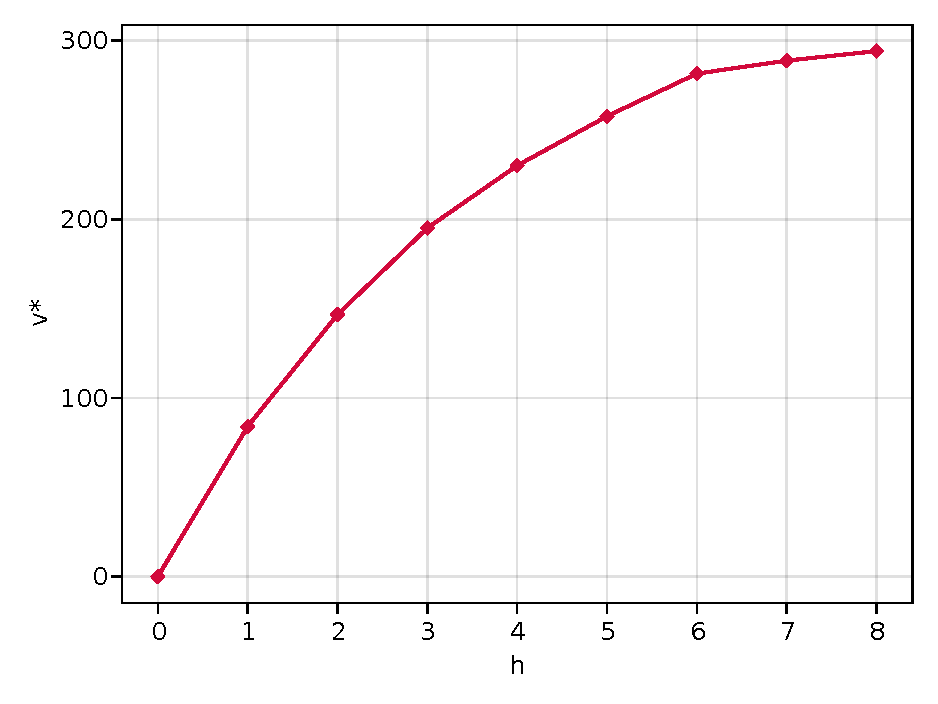
\includegraphics[width=0.95\textwidth]{./plots/h_v-example.pdf}
  \caption{  \label{planetsplot}
  \ifen Application limit $h$ versus the optimal portfolio valuation $v^* = v(\mathcal{X}_h)$ in a fictional market with $m=8$ schools. The concave shape suggests the result of Theorem \ref{concavityinh}. 
  \else $m=8$개의 학교로 구성된 가상 입학 시상에서, 각 지원 제한 $h$에 해당하는 최적 포트폴리오의 가치 $v^* = v(\mathcal{X}_h)$. 곡선의 오목성은 정리 \ref{concavityinh}의 결과를 시사한다.\fi}
\end{figure}








%\pagebreak
\ifen \section{Heterogeneous application costs} \else\section{동일하지 않은 지원 비용} \fi\label{hetappcosts}
\ifen
Now we turn to the more general problem in which the constant $g_j$ represents the \emph{cost} of applying to $c_j$ and the student, whom we now call Ellis, has a \emph{budget} of $H$ to spend on college applications.  Applying Lemma \ref{assumetzerozero}, we assume $t_0 = 0$ throughout.
\else
이제 $g_j$가 $c_j$에 지원하는 비용을 나타내며 학생이 지원에 쓸 수 있는 예산이 $H$인 일반적인 문제를 고려한다. 이 문제를 풀고자 하는 학생을 엘리스라고 부르자. 본 절 내내 기본 정리 \ref{assumetzerozero}을(를) 적용하여 $t_0 = 0$임을 가정하자.
\fi

\begin{problem}[\ifen Ellis's problem\else 엘리스의 문제\fi]
\ifen
Ellis's optimal college application portfolio is given by the solution to the following combinatorial optimization problem.
\else 
엘리스의 최적 대학 지원 포트폴리오는 다음 조합 최적화 문제의 최적해다.
\fi
\begin{align}
\begin{split}
\text{maximize}\quad &  v(\mathcal{X}) = \sum_{j\in
%\{0\}\cup
\mathcal{X}} \Bigl(f_j t_j \prod_{\substack{i \in \mathcal{X}: \\ i > j}} (1 - f_{i}) \Bigr)\\
\text{subject to}\quad & \mathcal{X}\subseteq\mathcal{C},~~\sum_{j \in \mathcal{X}} g_j \leq H 
\end{split}
\end{align}
\end{problem}

\ifen
\noindent In this section, we show that this problem is NP-complete, then provide four algorithmic solutions: an exact branch-and-bound routine, an exact dynamic program, a fully polynomial-time approximation scheme (FPTAS), and a simulated-annealing heuristic. 
\else
\noindent 본 절에서 이 문제가 NP-complete함을 보이고 3가지 해법을 제시한다: 정확한 분지한계법 해법, 정확한 동적 계획 해법, 완전 다항 시간 근사 해법(fully polynomial-time approximation scheme, FPTAS), 그리고 모의 담금질(simulated annealing) 휴리스틱.
\fi

\ifen \subsection{NP-completeness} \else \subsection{NP-completeness}\fi
\ifen
The optima for Ellis's problem are not necessarily nested, nor is the number of schools in the optimal portfolio necessarily increasing in $H$. For example, if
$f = (0.5, 0.5, 0.5)$, $t = (1, 1, 219)$, and $g = (1, 1, 3)$,
then it is evident that the optimal portfolio for $H = 2$ is $\{1, 2\}$ while that for $H = 3$ is $\{3\}$. In fact, Ellis’s problem is NP-complete, as we will show by a transformation from the binary knapsack problem, which is known to be NP-complete (Garey and Johnson 1979, \S\,3.2.1).
\else
엘리스 문제의 최적해는 필수적으로 포함 사슬 관계를 가지지 않으며 최적 포트폴리오에 속한 학교의 개수는 $H$에 대해 감소할 수도 있다. 예를 들어
$f = (0.5, 0.5, 0.5)$, $t = (1, 1, 219)$, 그리고 $g = (1, 1, 3)$이면 $H = 2$에 대응하는 최적해가 $\{1, 2\}$이며 $H = 3$에 대응하는 최적해는 $\{3\}$임을 쉽게 알 수 있다. 사실은 엘리스의 문제가 NP-complete하며 이를 이진 배낭 문제에서의 변환을 통해 증명할 수 있다. 배낭 문제의 NP-completeness가 이미 알려져 있다 (Garey and Johnson 1979, \S\,3.2.1).
\fi


\begin{problem}[\ifen Decision form of knapsack problem\else 배낭 문제의 결정 형태\fi]
\ifen 
An \emph{instance} consists of a set $\mathcal{B}$ of $m$ objects, utility values $u_j \in \mathbb{N}$ and weight $w_j \in \mathbb{N}$ for each $j \in \mathcal{B}$, and target utility $U\in \mathbb{N}$ and knapsack capacity $W\in \mathbb{N}$. The instance is called a \emph{yes-instance} if and only if there exists a set $\mathcal{B’} \subseteq \mathcal{B}$ having $\sum_{j \in \mathcal{B’}} u_j \geq U$ and  $\sum_{j \in \mathcal{B’}} w_j \leq W$.
\else
`인스턴스'는 $m$개 상품으로 이루어진 집합 $\mathcal{B}$, 각 $j \in \mathcal{B}$에 대한 효용값 $u_j \in \mathbb{N}$와 무게 $w_j \in \mathbb{N}$, 목적 효용 $U\in \mathbb{N}$, 그리고 배낭 용량 $W\in \mathbb{N}$로 구성된다. 인스턴스가 `예-인스턴스'가 될 필요충분 조건은 $\sum_{j \in \mathcal{B’}} u_j \geq U$와  $\sum_{j \in \mathcal{B’}} w_j \leq W$를 만족하는 집합 $\mathcal{B’} \subseteq \mathcal{B}$가 존재하는 것이다.
\fi
\end{problem}

\begin{problem}[\ifen Decision form of Ellis's problem\else 엘리스 문제의 결정 형태\fi] \label{ellisdecisionform}
\ifen
An \emph{instance} consists of an instance of Ellis’s problem and a target valuation $V$. The instance is called a \emph{yes-instance} if and only if there exists a portfolio $\mathcal{X} \subseteq \mathcal{C}$ having $v(\mathcal{X}) \geq V$ and  $\sum_{j \in \mathcal{X}} g_j \leq H$.
\else
`인스턴스'는 엘리스 문제의 인스턴스와 목적 포트폴리오 가치 $V$로 구성된다. 인스턴스가 `예-인스턴스'가 될 필요충분 조건은 $v(\mathcal{X}) \geq V$와 $\sum_{j \in \mathcal{X}} g_j \leq H$를 만족하는 포트폴리오 $\mathcal{X} \subseteq \mathcal{C}$가 존재하는 것이다.
\fi
\end{problem}

\begin{theorem}
\ifen
The decision form of Ellis’s problem is NP-complete.
\else
엘리스 문제의 결정 형태는 NP-complete하다.
\fi
\end{theorem}

\begin{proof}
\ifen It is obvious that the problem is in NP.
\else 문제가 NP에 속하는 것은 자명하다.\fi

\ifen
Consider an instance of the knapsack problem, and we will construct an instance of Problem \ref{ellisdecisionform} that is a yes-instance if and only if the corresponding knapsack instance is a yes-instance. Without loss of generality, we may assume that the objects in $\mathcal{B}$ are indexed in increasing order of $u_j$, that each $u_j >0$, and that each $w_j \leq W$. 
\else
임의의 배낭 문제 인스턴스를 택하고, 예-인스턴스 여부가 동치인 문제 \ref{ellisdecisionform}의 인스턴스를 만들자. 일반성을 잃지 않고 $\mathcal{B}$에 속한 상품이 $u_j$가 증가하는 순서대로 배열되며 모든 $u_j >0$이고 $w_j \leq W$임을 가정할 수 있다.
\fi

\ifen
Let $U_{\mathrm{max}} = \sum_{j \in \mathcal{B}} u_j$ and $\delta = {1} /{m U_{\mathrm{max}}} \in (0, 1)$, and construct an instance of Ellis’s problem with $\mathcal{C} = \mathcal{B}$, $H = W$, all $f_j = \delta$, and each $t_j = u_j / \delta$. Clearly, $\mathcal{X} \subseteq \mathcal{C}$ is feasible for Ellis’s problem if and only if it is feasible for the knapsack instance. Now, we observe that for any nonempty $\mathcal{X}$,
\else
$U_{\mathrm{max}} = \sum_{j \in \mathcal{B}} u_j$와 $\delta = {1} /{m U_{\mathrm{max}}} \in (0, 1)$일 때, $\mathcal{C} = \mathcal{B}$, $H = W$,  모든 $f_j = \delta$, 그리고 각 $t_j = u_j / \delta$인 엘리스 문제의 인스턴스를 고려하자. $\mathcal{X} \subseteq \mathcal{C}$가 엘리스 문제의 가능해가 되는 것은 배낭 문제 인스턴스의 가능해가 되는 것과 동치임을 쉽게 알 수 있다. 그러면 공집합이 아닌 임의의 $\mathcal{X}$ 에 대해,
\fi
\begin{align}
\begin{split}
\sum_{j \in \mathcal{X}} u_j &=  \sum_{j \in \mathcal{X}} f_j t_j
> \sum_{j \in \mathcal{X}} \Bigl( f_j t_j \prod_{\substack{j’ \in \mathcal{X}: \\ j' > j}} (1 - f_{j’}) \Bigr)
= v(\mathcal{X}) \\
&= \sum_{j \in \mathcal{X}} \Bigl( u_j  \prod_{\substack{j’ \in \mathcal{X}: \\ j' > j}} (1 - \delta) \Bigr)
\geq (1 - \delta)^m \sum_{j \in \mathcal{X}} u_j \\
&\geq (1 - m\delta) \sum_{j \in \mathcal{X}} u_j 
\geq \sum_{j \in \mathcal{X}} u_j  - m\delta U_{\mathrm{max}}
= \sum_{j \in \mathcal{X}} u_j  - 1.
\end{split}
\end{align}
\ifen
This means that the utility of an application portfolio $\mathcal{X}$ in the corresponding knapsack instance is the smallest integer greater than $v( \mathcal{X})$. That is, $\sum_{j \in \mathcal{X}} u_j \geq U$ if and only if $v(\mathcal{X}) \geq U -1$. Taking $V = U-1$ completes the transformation and concludes the proof. 
\else
이는 지원 포트폴리오 $\mathcal{X}$가 해당 배낭 문제에서 일으키는 효용이 $v( \mathcal{X})$보다 크면서 가장 작은 정수임을 의미한다. 즉, $\sum_{j \in \mathcal{X}} u_j \geq U$가 성립할 필요충분 조건은 $v(\mathcal{X}) \geq U -1$이다. $V = U-1$으로 정의하여 변환을 완성하면 증명이 완료된다.
\fi
\end{proof}

\ifen 
An intuitive extension of the greedy algorithm for Alma's problem is to iteratively add to $\mathcal{X}$ the school $k$ for which $\bigl( v(\mathcal{X}\cup\{k\}) - v(\mathcal{X}) \bigr) / g_k$ is largest. But the construction above shows that the objective function of Ellis's problem can approximate that of a knapsack problem with arbitrary precision. Therefore, in pathological examples such as the following, the greedy algorithm can achieve an arbitrarily small approximation ratio. 
\else
알마 문제를 위한 탐욕 해법의 직관적인 확장은 $\bigl( v(\mathcal{X}\cup\{k\}) - v(\mathcal{X}) \bigr) / g_k$-값이 가장 큰 학교 $k$를  $\mathcal{X}$에 차례대로 추가하는 것이다. 그러나 위에서 도출한 변환은 엘리스 문제의 목적함수를 배낭 문제의 목적함수의 원하는 만큼 정확한 근사로 만들 수 있음을 의미한다. 따라서 다음 같은 병례에서 탐욕 해법은 임의로 낮은 근사 비율을 일으킬 수 있다.
\fi
\begin{example} \label{greedyzeroellis}
\ifen
Let $t = (10, 2021)$, $f = (0.1, 0.1)$, $g = (1, 500)$, and $H = 500$. Then the greedy approximation algorithm produces the clearly suboptimal solution $\mathcal{X} = \{1\}$. 
\else
 $t = (10, 2021)$, $f = (0.1, 0.1)$, $g = (1, 500)$, 그리고 $H = 500$이라고 하자. 그러면 탐욕 해법은 $\mathcal{X} = \{1\}$을 출력하며 이는 분명히 최적해가 아니다.
\fi
\end{example} 
\ifen
We might expect to obtain a better approximate solution to Ellis's problem by solving the following knapsack problem (nevermind that it is NP-complete) as a surrogate.
\begin{equation}
\text{maximize}\quad \sum_{j \in \mathcal{X}} f_j t_j \qquad \text{subject to}\quad\mathcal{X}\subseteq\mathcal{C},~~\sum_{j \in \mathcal{X}} g_j \leq H
\end{equation}
However, upon inspection, this solution merely generalizes the na\"ive algorithm for Alma's problem (Definition \ref{naivealgorithm}). In Ellis's problem, because the number of schools in the optimal portfolio can be as large as $m-1$, the knapsack solution's approximation coefficient is $1/(m-1)$ by analogy with \eqref{oneoverhopt}. A tight example is as follows. 
\else
엘리스 문제의 좀 더 좋은 근사해를 찾기 위해 다음 배낭 문제를 (NP-complete함을 무시하고) 대리 문제로 푸는 것에 매력은 있다.
\begin{equation}
\text{maximize}\quad \sum_{j \in \mathcal{X}} f_j t_j \qquad \text{subject to}\quad\mathcal{X}\subseteq\mathcal{C},~~\sum_{j \in \mathcal{X}} g_j \leq H
\end{equation}
그러나 이러한 해법은 사실 알마 문제의 나이브 해법(정의 \ref{naivealgorithm})의 단순한 일반화임을 알 수 있다. 엘리스 문제에서 최적 포트폴리오에 크기가 $m-1$이 될 수 있으므로 배낭 문제 해법의 근사 계수는 \eqref{oneoverhopt}과(와) 유사하듯이 $1 / (m-1)$이다. 타이트한 예는 다음과 같다.
\fi
\begin{example} \label{knapsackheuristicellis}
\ifen Consider the following instance of Ellis's problem, where $H = m-1$.
\else 엘리스 문제의 다음 인스턴스를 고려하자. 단, $H = m-1$이다. \fi
\begin{center}
\begin{tabular}{r|cccc}
$j$   & $1$            & $\cdots$ & $m-1$          & $m$            \\ \hline
$f_j$ & $1$            &  $\cdots$ & $1$            & $\frac{1}{m-1}$ \\
$t_j$ & $\frac{1}{m-1}$ &  $\cdots$ & $\frac{1}{m-1}$ & $m-1$          \\
$g_j$ & $1$            &  $\cdots$ & $1$            & $m-1$         
\end{tabular}%
\end{center}
\ifen
The feasible solutions $\mathcal{Y} = \{1, \dots, m-1\}$ and $\mathcal{X} = \{ m\}$ each have $\sum_{j \in \mathcal{Y}} f_j t_j = \sum_{j \in \mathcal{X}} f_j t_j =  1$, and thus the knapsack algorithm can choose $\mathcal{Y}$ with $v(\mathcal{Y}) = 1/(m-1)$. But the optimal solution is  $\mathcal{X}$ with $v(\mathcal{X}) =  1$. 
\else
가능해 $\mathcal{Y} = \{1, \dots, m-1\}$와 $\mathcal{X} = \{ m\}$에 대해 $\sum_{j \in \mathcal{Y}} f_j t_j = \sum_{j \in \mathcal{X}} f_j t_j =  1$이므로 배낭 문제 해법은  $\mathcal{Y}$를 선택할 수 있다. 그의 가치는 $v(\mathcal{Y}) = 1/(m-1)$이다. 그러나 $\mathcal{X}$는 최적해이며 그의 가치는 $v(\mathcal{X}) =  1$이다.
\fi
\end{example}

\ifen 
In summary, neither a greedy algorithm nor a knapsack-based algorithm solves Ellis's problem to optimality. 
\else
탐욕 해법 또는 배낭 문제 기반 해법으로 엘리스 문제의 정확한 최적해를 구할 수 없음을 의미한다.
\fi


\ifen \subsection{Branch-and-bound algorithm} \else \subsection{분지한계법} \fi \label{subsectionbranchbound}
\ifen 
A traditional approach to integer optimization problems is the branch-and-bound framework, which generates subproblems in which the values of one or more decision variables are fixed and uses an upper bound on the objective function to exclude, or \emph{fathom,} branches of the decision tree that cannot yield a solution better than the best solution on hand (Martello and Toth 1990; Kellerer et al. 2004). In this subsection, we present an integer formulation of Ellis's problem and a linear program (LP) that bounds the objective value from above. We tighten the LP bound for specific subproblems by reusing the conditional transformation of the $t_j$-values from Algorithm \ref{algorithmforlargeh}. A branch-and-bound routine emerges naturally from these ingredients.
\else
정수 최적화의 고전적인 기법 중 분지한계법(branch and bound)이 있다. 이는 하나 이상의 결정 변수를 고정하고 해당 부문제를 탐색하는 해법이며, 목적함수의 상한(bound)을 활용하여 기존 해보다 좋은 해를 생성할 수 없는 결정 나무의 가지(branch)를 제외하여 결정 공간을 줄인다 (Martello and Toth 1990; Kellerer 외 2004). 본 항에서, 엘리스 문제의 정수 모형과 그의 상한이 되는 선형 계획을 제시한다. 알고리즘 \ref{algorithmforlargeh}에서 개발한 $t_j$-값의 변환을 활용하여 부문제의 선형 완화 문제에 의한 상한을 더 타이트하게 만든다. 이 기반으로 분지한계법 알고리즘을 도출한다.
\fi

\ifen
To begin, let us characterize the portfolio $\mathcal{X}$ as the binary vector $x \in \{0, 1\}^m$, where $x_j = 1 $ if and only if $j \in \mathcal\{X\}$. Then it is not difficult to see that Ellis's problem is equivalent to the following integer nonlinear program. 
\else
우선 포트폴리오 $\mathcal{X}$를 이진 특성 벡터 $x \in \{0, 1\}^m$로 표현하자. 단, $x_j = 1 $인 것은 $j \in \mathcal\{X\}$과 동치다. 그러면 엘리스의 문제가 다음 비선형 정수 최적화 문제와 동등함을 볼 수 있다.
\fi
\begin{problem}[\ifen Integer NLP for Ellis's problem\else 엘리스의 문제를 위한 비선형 정수 계획\fi] \label{integernlp}
\begin{align}
\begin{split}
\text{maximize}\quad &  v(x) = \sum_{j=1}^m \Bigl(f_j t_j  x_j \prod_{i > j} (1 - f_{i} x_i) \Bigr)\\
\text{subject to}\quad & \sum_{j=1}^m g_j x_j \leq H, ~~ x_i \in \{0, 1\}^m
\end{split}
\end{align}
\end{problem}
\ifen
\noindent Since the product in $v(x)$ does not exceed one, the following LP relaxation is an upper bound on the valuation of the optimal portfolio.
\else
\noindent $v(x)$에서 등장하는 곱은 1을 넘을 수 없으므로 다음 선형 완화 문제는 최적 포트폴리오 가치의 상한이 된다.
\fi
\begin{problem}[\ifen LP relaxation for Ellis's problem\else 엘리스의 문제를 위한 선형 완화 문제\fi] \label{LPrelaxation}
\begin{align}
\begin{split}
\text{maximize}\quad &  v_{\mathrm{LP}}(x) = \sum_{j=1}^m  f_j t_j x_j \\
\text{subject to}\quad & \sum_{j=1}^m g_j x_j \leq H, ~~ x \in [0, 1]^m
\end{split}
\end{align}
\end{problem}
\ifen
\noindent Problem \ref{LPrelaxation} is a continuous knapsack problem, which is easily solved in $O(m \log m)$ time by a greedy algorithm (Dantzig 1957). Balas and Zemel (1980, \S\,2) provide an $O(m)$ algorithm. 
\else
\noindent 문제 \ref{LPrelaxation}은(는) ``연속 배낭 문제''라고 불리며 탐욕 알고리즘을 적용하면 $O(m \log m)$ 시간에 쉽게 풀 수 있다 (Dantzig 1957).  $O(m)$ 알고리즘도 알려져 있다 (Balas와 Zemel 1980, \S\,2).
\fi

\ifen In our branch-and-bound framework, a \emph{node} is characterized by a three-way partition of schools $\mathcal{C}= \mathcal{I} \cup \mathcal{O} \cup \mathcal{N}$ satisfying $\sum_{j \in \mathcal{I}} g_j \leq H$. $\mathcal{I}$ consists of schools that are ``in'' the application portfolio ($x_j = 1$), $\mathcal{O}$ consists of those that are ``out'' ($x_j = 0$), and $\mathcal{N}$ consists of those that are ``negotiable.'' 
%This partition induces a constant $\gamma$, transformed $t_j$-values $\bar t$, the residual budget $\mathcal{H}$, and a set $\mathcal{L}$ of pointers to the node's children, if any.
The choice of partition induces a pair of subproblems. The first subproblem is an instance of Problem \ref{integernlp}, namely
\else
본 연구의 분지한계법 설계에서, `마디'(node)는 학교를 세 군으로 나눈 분할 $\mathcal{C}= \mathcal{I} \cup \mathcal{O} \cup \mathcal{N}$로 묘사한다. 단, $\mathcal{I}$는 $\sum_{j \in \mathcal{I}} g_j \leq H$을 만족한다. $\mathcal{I}$는 지원 포트폴리오에 속한 학교(`in': $x_j = 1$), $\mathcal{O}$는 속하지 않은 학교(`out': $x_j = 0$), 그리고 $\mathcal{N}$은 미결의 학교(`negotiable')로 이루어진다. 분할이 결정되면 부문제의 한 쌍이 결정해진다. 첫 번째 부문제는 다음 같은 문제 \ref{integernlp}의 인스턴스다.
\fi
\begin{align} \label{nodenlpsubproblem}
\begin{split}
\text{maximize}\quad &  v(x) = \gamma + \sum_{j \in \mathcal{N}} \Bigl(f_j \bar t_j x_j \prod_{\substack{i \in \mathcal{N}:\\i > j}} (1 - f_{i} x_i) \Bigr)\\
\text{subject to}\quad & \sum_{j \in \mathcal{N}} g_j x_j \leq \bar H; ~~ x_j \in \{0, 1\},~~j \in \mathcal{N}.
\end{split}
\end{align}
\ifen The second is the corresponding instance of Problem \ref{LPrelaxation}:
\else 두 번째 부문제는 대응하는 문제 \ref{LPrelaxation} 인스턴스다.\fi
\begin{align} \label{nodelprelaxation}
\begin{split}
\text{maximize}\quad &  w_{\mathrm{LP}}(x)= \gamma + \sum_{j \in \mathcal{N}}  f_j \bar t_j  x_j \\
\text{subject to}\quad & \sum_{j \in \mathcal{N}} g_j x_j \leq \bar H; ~~ x_j \in [0, 1],~~j \in \mathcal{N}
\end{split}
\end{align}
\ifen
In both subproblems, $\bar H = H - \sum_{j\in \mathcal{I}} g_j$ denotes the residual budget. The parameters $\gamma$ and $\bar t$ are obtained by iteratively applying the transformation \eqref{howtotransformtj} to the schools in $\mathcal{I}$. For each $j\in \mathcal{I}$,  we increment $\gamma$ by the current value of $f_j \bar t_j$, eliminate $j$ from the market, and update the remaining $\bar t_j$-values using \eqref{howtotransformtj}. (An example is given below.)
\else
각 부문제에서 $\bar H = H - \sum_{j\in \mathcal{I}} g_j$는 잔여 예산을 의미한다. $\mathcal{I}$에 속한 학교에 \eqref{howtotransformtj}의 변환을 적용하여 모수 $\gamma$와 $\bar t$를 얻을 수 있다. 즉, 각 $j\in \mathcal{I}$에 대해 $\gamma$를 $f_j \bar t_j$ 만큼 증가시키고, 시장에서 $j$를 소거하고, \eqref{howtotransformtj}에 따라 남은 $\bar t_j$-값을 수정한다. (아래에서 예를 제시한다.)
\fi

\ifen 
Given a node $n  = (\mathcal{I}, \mathcal{O}, \mathcal{N})$, its children are generated as follows. Every node has two, one, or zero children. In the typical case, we select a school $j \in \mathcal{N}$ for which $g_j \leq \bar H$ and generate one child by moving $j$ to $\mathcal{I}$, and another child by moving $j$ it to $\mathcal{O}$. Equivalently, we set $x_j = 1$ in one child and $x_j = 0$ in the other. In principle, any school can be chosen for $j$, but as a greedy heuristic, we choose the school for which the ratio $f_j \bar t_j / g_j$ is highest. Notice that this method of generating children ensures that each node's $\mathcal{I}$-set differs from its parent's by at most a single school, so the constant $\gamma$ and transformed $\bar t_j$-values for the new node can be obtained by a single application of \eqref{howtotransformtj}. 
\else
마디  $n  = (\mathcal{I}, \mathcal{O}, \mathcal{N})$이 주어질 때, 그의 새끼 마디를 다음처럼 생성한다. 모든 마디에는 2, 1, 혹은 0개의 새끼가 있다. 전형적인 경우에서, $g_j \leq \bar H$를 만족하는 학교 $j \in \mathcal{N}$ 선택한다. $j$를 $\mathcal{I}$로 이동시켜서 한 새끼를 얻고, $j$를 $\mathcal{O}$로 이동시켜서 다른 새끼를 얻는다. 즉, 한 새끼 마디에서 $x_j = 1$로 고정하고 다른 새끼 마디에서 $x_j = 0$으로 고정한다. 일반적으로 $j$는 임의의 학교가 될 수 있지만 탐욕적인 휴리스틱으로 $f_j \bar t_j / g_j$의 비율이 가장 큰 학교를 선택한다. 이런 식으로 새끼를 생성하면 각 마디의 $\mathcal{I}$-집합은 자기 어미 마디의 $\mathcal{I}$-집합과 최대 한 학교로만 다르다. 따라서 새로운 마디를 생성할 때, \eqref{howtotransformtj}을(를) 한 번만 적용하면 상수 $\gamma$와 변화된 $\bar t_j$-값을 얻을 수 있다.
\fi

\ifen
There are two atypical cases. First, if every school in $\mathcal{N}$ has $g_j > \bar H$, then there is no school that can be added to $\mathcal{I}$ in a feasible portfolio, and the optimal portfolio on this branch is $\mathcal{I}$ itself. In this case, we generate only one child by moving all the schools from $\mathcal{N}$ to $\mathcal{O}$. Second, if $\mathcal{N} = \O$, then the node has zero children, and as no further branching is possible, the node is called a \emph{leaf.}
\else
이례적인 경우 2가지 있다. 첫 번째는, $\mathcal{N}$에 속한 모든 학교에 대해 $g_j > \bar H$이면 가능성을 유지하며 $\mathcal{I}$에 추가할 수 있는 학교가 없으므로 본 가지의 최적 포트폴리오는 단지 $\mathcal{I}$ 자체다. 이때 $\mathcal{N}$에 원소를 모두 $\mathcal{O}$로 이동시켜서 단일 새끼를 생성한다. 두 번째는, $\mathcal{N} = \O$인 마디는 새끼가 없다. 더 이상 분지할 수 없으므로 이 마디를 `잎 마디'(leaf)라고 한다.
\fi

\begin{example}
\ifen
Consider a market in which $t = (20, 40, 60, 80, 100)$, $f = (0.5, 0.5, 0.5, 0.5, 0.5)$, $g = (3, 2, 3, 2, 3)$, and $H = 8$, and the node $n =  (\mathcal{I}, \mathcal{O}, \mathcal{N}) = (\{2, 5\}, \{1\}, \{3, 4\})$. Let us compute the two subproblems associated with $n$ and identify its children. To compute the subproblems, we first simply disregard $c_1$. Next, to eliminate $c_2$, we apply \eqref{howtotransformtj} to $t$ to obtain
$\{\bar{\bar t}_3, \bar{\bar t}_4, \bar{\bar t}_5\} = \{ (1 - f_2) t_3, (1 - f_2) t_4, (1 -f_2) t_5\} = \{30, 40, 50 \}$ and $\bar{\bar \gamma} = f_2 t_2 = 20$. We eliminate $c_5$ by again applying \eqref{howtotransformtj} to $\bar{ \bar t}$ to obtain $\{\bar t_3, \bar t_4\} =  \{\bar{\bar t}_3 - f_5 \bar{\bar t}_5, \bar{\bar t}_4-  f_5 \bar{\bar t}_5\}= \{5, 15\}$ and $\gamma = \bar{\bar \gamma} + f_5 \bar{\bar t}_5 = 35$. Finally, $\bar H = H - g_2 - g_5 = 3$. Now problems \eqref{nodenlpsubproblem} and \eqref{nodelprelaxation} are easily obtained by substitution.
\else
 $t = (20, 40, 60, 80, 100)$, $f = (0.5, 0.5, 0.5, 0.5, 0.5)$, $g = (3, 2, 3, 2, 3)$, 그리고 $H = 8$인 시장과 마디 $n =  (\mathcal{I}, \mathcal{O}, \mathcal{N}) = (\{2, 5\}, \{1\}, \{3, 4\})$이 주어질 때 $n$에 대응하는 부문제와 새끼 마디를 구하자. 부문제를 계산하기 위해 먼저 $c_1$을 단순히 무시한다.  $c_2$를 소거하기 위해 $t$에 \eqref{howtotransformtj}에 적용하여 
$\{\bar{\bar t}_3, \bar{\bar t}_4, \bar{\bar t}_5\} = \{ (1 - f_2) t_3, (1 - f_2) t_4, (1 -f_2) t_5\} = \{30, 40, 50 \}$과 $\bar{\bar \gamma} = f_2 t_2 = 20$을 얻는다. $c_5$를 소거하기 위해 $\bar{\bar t}$에 \eqref{howtotransformtj}에 다시 적용하여 $\{\bar t_3, \bar t_4\} =  \{\bar{\bar t}_3 - f_5 \bar{\bar t}_5, \bar{\bar t}_4-  f_5 \bar{\bar t}_5\}= \{5, 15\}$와 $\gamma = \bar{\bar \gamma} + f_5 \bar{\bar t}_5 = 35$를 얻는다. 마지막으로, $\bar H = H - g_2 - g_5 = 3$이다. 이제 \eqref{nodenlpsubproblem}과(와) \eqref{nodelprelaxation}인 부문제를 쉽게 구할 수 있다.
\fi

\ifen
Since at least one of the schools in $\mathcal{N}$ has $g_j \leq \bar H$, $n$ has two children. Applying the node-generation rule, $c_4$ has the highest $f_j \bar t_j / g_j$-ratio, so the children are $n_1 = (\{2, 4, 5\}, \{1\}, \{3\})$ and $n_2 = (\{2, 5\}, \{1, 4\}, \{3\})$.
\else
$\mathcal{N}$에 속한 학교 중에 $g_j \leq \bar H$인 학교가 있으므로 $n$은 새끼 마디 2개 있다. $f_j \bar t_j / g_j$-비율이 가장 큰 학교는 $c_4$이므로 새끼 마디를 생성하는 법칙을 적용하면 $n_1 = (\{2, 4, 5\}, \{1\}, \{3\})$과 $n_2 = (\{2, 5\}, \{1, 4\}, \{3\})$ 같은 새끼를 얻는다.
\fi
\end{example}

\ifen
To implement the branch-and-bound algorithm, we represent the set of candidate nodes---namely, nonleaf nodes whose children have not yet been generated---by $\mathfrak{T}$. Each time a node $n= (\mathcal{I}, \mathcal{O}, \mathcal{N})$ is generated, we record the values $v_{\mathcal{I}}[n] = v(\mathcal{I})$ and $v^*_{\mathrm{LP}}[n]$, the optimal objective value of the LP relaxation \eqref{nodelprelaxation}. Because $\mathcal{I}$ is a feasible portfolio, $v_{\mathcal{I}}[n]$ is a lower bound on the optimal objective value. Moreover, by the argument given in the proof of Theorem \ref{nestedapplication}, the objective function of  \eqref{nodenlpsubproblem} is identical to the function $v(\mathcal{I} \cup \mathcal{X})$. This means that $v_{\mathrm{LP}}^*[n]$  is an upper bound on the valuation of any portfolio that contains $\mathcal{I}$ as a subset and does not include any school in $\mathcal{O}$, and hence on the valuation of any portfolio on this branch. Therefore, if upon generating a new node $n_2$, we discover that its objective value $v_{\mathcal{I}}[n_2]$ is greater than $v_{\mathrm{LP}}^*[n_1]$ for some other node $n_1$, then we can disregard $n_1$ and all its descendants. 
\else
분지한계법을 실행하기 위해 후보 마디, 즉 잎이 아니면서 새끼를 아직 생성하지 않은 마디의 집합을  $\mathfrak{T}$라고 부르자. 마디 $n= (\mathcal{I}, \mathcal{O}, \mathcal{N})$를 생성할 때마다, $v_{\mathcal{I}}[n] = v(\mathcal{I})$과 선형 완화 문제 \eqref{nodelprelaxation}의 최댓값 $v^*_{\mathrm{LP}}[n]$를 기록한다. $\mathcal{I}$는 예산에 가능한 포트폴리오이므로 $v_{\mathcal{I}}[n]$는 원래 목적함수 최댓값의 하한이 된다. 또한 정리 \ref{nestedapplication}의 증명 과정에서 보였듯, \eqref{nodenlpsubproblem}의 목적함수는 함수 $v(\mathcal{I} \cup \mathcal{X})$과 동치다. 이는 $v_{\mathrm{LP}}^*[n]$는 $\mathcal{I}$를 부분집합으로 포함하며 $\mathcal{O}$에 속한 학교를 포함하지 않은, 즉 이 가지에 있는 모든 포트폴리오의 가치에 대한 상한임을 의미한다. 따라서 새로운 마디 $n_2$를 생성했을 때, 만약 그의 목적 함숫값 $v_{\mathcal{I}}[n_2]$가 어떤 다른 마디 $n_1$에 대응하는 $v_{\mathrm{LP}}^*[n_1]$보다 크다면, $n_1$과 그의 모든 후손을 무시할 수 있다.
\fi

\ifen
The algorithm is initialized by populating $\mathfrak{T}$ with the root node $n_0 = (\O, \O, \mathcal{C})$. At each iteration, it selects the node $n \in \mathfrak{T}$ having the highest $v_{\mathrm{LP}}^*[n]$-value, generates its children, and removes $n$ from the candidate set. Next, the children $n'$ of $n$ are inspected and added to the tree. If one of the children yields a new optimal solution, then we mark it as the best candidate and fathom any nodes $n''$ for which  $v_{\mathcal{I}}[n'] >  v_{\mathrm{LP}}^*[n'']$. When no nodes remain in the candidate set, the algorithm has explored every branch, so it returns the best candidate and terminates.
\else
$\mathfrak{T}$에 뿌리 마디 $n_0 = (\O, \O, \mathcal{C})$를 넣어서 알고리즘을 초기화한다. 각 반복 단계에서 $v_{\mathrm{LP}}^*[n]$-값이 가장 큰 마디 $n \in \mathfrak{T}$을 선택한다. $n$의 새끼를 생성하고 후보 집합에서 제거한다. 그다음에 $n$의 각 새끼 마디 $n'$을 검증하고 나무에 추가한다. 새끼 마디 중에 새로운 최적해를 발견하면 이를 가장 좋은 후보로 표하고  $v_{\mathcal{I}}[n'] >  v_{\mathrm{LP}}^*[n'']$인 마디 $n''$을 후보 집합에서 제거한다. 후보 집합이 공집합이 되면 알고리즘이 모든 가지를 탐색했으므로 가장 좋은 후보를 출력하고 종료한다.
\fi


\ifen {
\begin{algorithm}[h] 
%\DontPrintSemicolon
\caption{Branch and bound for Ellis's problem.} \label{ellisbnb}
\KwIn{Utility values $t \in(0, \infty)^m$, admissions probabilities $f \in (0, 1]^m$, application costs $g \in (0, \infty)^m$, budget $H \in (0, \infty)$.}
Root node $n_0 \gets (\O, \O, \mathcal{C})$\;
Current lower bound $L \gets 0$ and best solution $\mathcal{X} \gets \O$\;
Candidate set $\mathfrak{T} \gets \{ n_0\}$\;
\While{not finished}{
	\lIf{$\mathfrak{T} = \O$}{\Return{$\mathcal{X}, L$}}
	\Else{
		$n \gets \argmax\{ v_{\mathrm{LP}}^*[n] : n \in \mathfrak{T}\}$\;
		Remove $n$ from $\mathfrak{T}$\;
%		Generate children of $n$\;
		\For{each child $n'$ of $n$}{
			\If{$L < v_{\mathcal{I}}[n']$}{
				$L \gets v_{\mathcal{I}}[n']$\;
				Update $\mathcal{X}$ to the $\mathcal{I}$-set associated with $n'$\;
			}
			\lIf{$v_{\mathrm{LP}}^*[n] > L$ and $n'$ is not a leaf}{add $n'$ to $\mathfrak{T}$}
		}
		\For{$n'' \in \mathfrak{T}$} {
			\lIf{$L >  v_{\mathrm{LP}}^*[n'']$}{remove $n''$ from $\mathfrak{T}$}
		}
	}
}
\end{algorithm}
} \else {
\begin{algorithm}[h] 
%\DontPrintSemicolon
\caption{엘리스의 문제를 위한 분지한계법.} \label{ellisbnb}
\KwIn{효용 모수 $t \in(0, \infty)^m$, 합격 확률 $f \in (0, 1]^m$, 지원 비용 $g \in (0, \infty)^m$, 예산 $H \in (0, \infty)$.}
뿌리 마디 $n_0 \gets (\O, \O, \mathcal{C})$\;
현재 하한 $L \gets 0$ 및 최적해 $\mathcal{X} \gets \O$\;
후보 집합 $\mathfrak{T} \gets \{ n_0\}$\;
\While{종료되지 않음}{
	\lIf{$\mathfrak{T} = \O$}{\Return{$\mathcal{X}, L$}}
	\Else{
		$n \gets \argmax\{ v_{\mathrm{LP}}^*[n] : n \in \mathfrak{T}\}$\;
		$\mathfrak{T}$에서 $n$을 제거\;
%		Generate children of $n$\;
		\For{$n$의 각 새끼 마디 $n'$}{
			\If{$L < v_{\mathcal{I}}[n']$}{
				$L \gets v_{\mathcal{I}}[n']$\;
				$\mathcal{X}$을 $n'$에 대응하는 $\mathcal{I}$-집합으로 수정\;
			}
			\lIf{$v_{\mathrm{LP}}^*[n] > L$이고 $n'$이 잎 마디 아님}{$\mathfrak{T}$에 $n'$을 추가}
		}
		\For{$n'' \in \mathfrak{T}$} {
			\lIf{$L >  v_{\mathrm{LP}}^*[n'']$}{$\mathfrak{T}$에서 $n''$을 제거}
		}
	}
}
\end{algorithm}
} \fi

\begin{theorem}[\ifen Validity of Algorithm \ref{ellisbnb}\else 알고리즘 \ref{ellisbnb}의 타당성\fi]
\ifen Algorithm \ref{ellisbnb} produces an optimal application portfolio for Ellis's problem.
\else 알고리즘 \ref{ellisbnb}은(는) 엘리스 문제의 최적 지원 포트폴리오를 출력한다. \fi
\end{theorem}

\begin{proof}
\ifen
Because an optimal solution exists among the leaves of the tree, the discussion above implies that as long as the algorithm terminates, it returns an optimal solution.

To show that the algorithm does not cycle, it suffices to show that no node is generated twice. Suppose not: that two distinct nodes $n_1$ and $n_2$ share the same partition $(\mathcal{I}_{12}, \mathcal{O}_{12}, \mathcal{N}_{12})$. Trace each node's lineage up the tree and let $n$ denote the \emph{first} node at which the lineages meet. $n$ must have two children, or else its sole child is a common ancestor of $n_1$ and $n_2$, and one of these children, say $n_3$, must be an ancestor of $n_1$ while the other, say $n_4$, is an ancestor of $n_2$.  Write $n_3 = (\mathcal{I}_{3}, \mathcal{O}_{3}, \mathcal{N}_{3})$ and $n_4 = (\mathcal{I}_{4}, \mathcal{O}_{4}, \mathcal{N}_{4})$. By the node-generation rule, there is a school $j$ in $\mathcal{I}_3 \cap \mathcal{O}_4$, and the $\mathcal{I}$-set (respectively, $\mathcal{O}$-set) for any descendant of $\mathcal{I}_3$ (respectively, $\mathcal{O}_4$) is a superset of  $\mathcal{I}_3$ (respectively, $\mathcal{O}_4$). Therefore, $j \in \mathcal{I}_{12} \cap \mathcal{O}_{12}$, meaning that $(\mathcal{I}_{12}, \mathcal{O}_{12}, \mathcal{N}_{12})$ is not a partition of $\mathcal{C}$, a contradiction. 
\else
나무의 잎 마디 중 최적해가 반드시 존재하므로 위의 논의에 따라 알고리즘이 종료한다면 최적해를 출력하는 것을 알 수 있다.

알고리즘에서 회로가 생기지 않음을 보이기 위해 어떤 한 마디가 두 번 생성되지 않는 것을 증명하면 충분하다. 모순을 보이기 위해 같은 분할 $(\mathcal{I}_{12}, \mathcal{O}_{12}, \mathcal{N}_{12})$를 가지는 상이한 마디 $n_1$과 $n_2$가 생성된다고 하자. 나무에 올라가면서 두 마디의 가계가 서로 만나는 첫 마디를 $n$이라고 하자. $n$은 새끼 마디 하나만 가지면 그 자체가  $n_1$과 $n_2$의 공통 선조가 되며 이는 모순이므로 $n$ 새끼의 개수가 2임을 알 수 있다. 또한 그중 하나는 $n_1$의 선조며 다른 하나는 $n_2$의 선조다. 각각 $n_3 = (\mathcal{I}_{3}, \mathcal{O}_{3}, \mathcal{N}_{3})$ 그리고 $n_4 = (\mathcal{I}_{4}, \mathcal{O}_{4}, \mathcal{N}_{4})$라고 하자. 마디 생성 규칙에 따라 $\mathcal{I}_3 \cap \mathcal{O}_4$에 속한 학교 $j$가 존재하며,  $\mathcal{I}_3$ ($\mathcal{O}_4$)의 모든 후손 마디의 $\mathcal{I}$-집합 ($\mathcal{O}$-집합)은  $\mathcal{I}_3$ ($\mathcal{O}_4$)의 확대 집합이다. 따라서 $j \in \mathcal{I}_{12} \cap \mathcal{O}_{12}$가 되며 이는 $(\mathcal{I}_{12}, \mathcal{O}_{12}, \mathcal{N}_{12})$가 $\mathcal{C}$의 분할이 아님을 의미한다. 모순. 
\fi
\end{proof}

\ifen
The branch-and-bound algorithm is an interesting benchmark, but as a kind of enumeration algorithm, its computation time grows rapidly in the problem size, and unlike the approximation scheme we propose later on, there is no guaranteed bound on the approximation error after a fixed number of iterations. Moreover, when there are many schools in $\mathcal{N}$, the LP upper bound may be much higher than $v_{\mathcal{I}}[n']$. This means that significant fathoming operations do not occur until the algorithm has explored deep into the tree, at which point the bulk of the computational effort has already been exhausted. In our numerical experiments, Algorithm \ref{ellisbnb} was ineffective on instances larger than about $m=35$ schools, and therefore it does not represent a significant improvement over na\"ive enumeration. We speculate that the algorithm can be improved by incorporating cover inequalities (Wolsey 1998, \S\,9.3).  
\else
분지한계법은 기술적으로 유리한 기준점이지만, 일종의 열거 해법이므로 계산 시간이 문제 크기와 지수적으로 늘어난다. 그리고 뒤에서 제안하는 근사 해법과 달리, 주어진 반복한계의 개수에 대한 정확성 보장이 없다. 또한 $\mathcal{N}$에 학교가 많을 때, 선형 완화 문제 상한은 $v_{\mathcal{I}}[n']$보다 매우 높을 수도 있다. 이는 해법이 나무에 어느 정도 깊게 파고들어야 마디를 제외할 수 있음을 의미하며, 그때 계산 노력의 대부분은 이미 쏟은 것이다. 수리 실험에서, 알고리즘 \ref{ellisbnb}은(는) 약 $m=35$개의 학교를 넘는 인스턴스에 대해 비효율적이었으며 이는 단순한 열거법에 비해 큰 개선이 아니다. 하지만, 커버 부등식을 도입하여 해법을 개선할 가능성이 보인다 (Wolsey 1998, \S\,9.3).
\fi





\ifen \subsection{Pseudopolynomial-time dynamic program} \else\subsection{의사 다항 시간 동적 계획} \fi
\ifen
In this subsection, we assume, with a small loss of generality, that $g_j \in \mathbb{N}$ for $j = 1\dots m$ and $H \in\mathbb{N}$, and provide an algorithmic solution to Ellis's problem that runs in $O(Hm + m\log m)$ time. The algorithm resembles a familiar dynamic programming algorithm for the binary knapsack problem (Dantzig 1957; \emph{Wikipedia}, s.v. ``Knapsack problem''). Because we cannot assume that $H \leq m$ (as was the case in Alma's problem), this represents a pseudopolynomial-time solution (Garey and Johnson 1979, \S\,4.2). However, it is quite effective for typical college-application instances in which the application costs are small integers.
\else
본 절에서 일반성을 약간 제한하여 $g_j \in \mathbb{N}$ for $j = 1\dots m$과 $H \in\mathbb{N}$임을 가정한다. 이때 엘리스의 문제를 위한 $O(Hm + m\log m)$ 시간 해법을 제시한다. 해법은 이진 배낭 문제를 위한 익숙한 동적 계획 해법과 비슷하다 (Dantzig 1957; \emph{Wikipedia}, s.v. ``Knapsack problem''). 알마의 문제와 달리, 여기에서 $H \leq m$임을 가정할 수 없으므로 이는 의사 다항 시간 해법이라고 한다 (Garey and Johnson 1979, \S\,4.2). 그러나 지원 비용이 작은 정수가 되는 전형적인 대학 지원 문제 인스턴스에 대해 매우 효율적인 해법이다.
\fi

\ifen 
For $j = 0 \dots m$ and $h = 0 \dots H$, let $\mathcal{X}[j, h]$ denote the optimal portfolio using only the schools $\{ 1, \dots, j\}$ and costing no more than $h$, and let $V[j,h] = v(\mathcal{X}[j, h])$.  It is clear that if $j=0$ or $h=0$, then $\mathcal{X}[j, h] = \O$ and $V[j, h] = 0$.  For convenience, we also define $V[j, h] = -\infty$ for all $h < 0$.
\else
$j = 0 \dots m$와 $h = 0 \dots H$에 대해, $\{ 1, \dots, j\}$에 속한 학교만 사용하면서 지원 지출액이 $h$을 넘지 않는 최적 포트폴리오를 $\mathcal{X}[j, h]$라고 하자. 또한  $V[j,h] = v(\mathcal{X}[j, h])$다. $j=0$ 혹은 $h=0$이면 $\mathcal{X}[j, h] = \O$이고 $V[j, h] = 0$이 되는 것은 분명하다. 편의상 $h < 0$이면 $V[j, h] = -\infty$이라고 정의하자.
\fi

\ifen
For the remaining indices, $\mathcal{X}[j, h]$ either contains $j$ or not. If it does not contain $j$, then $\mathcal{X}[j, h] = \mathcal{X}[j-1, h]$. On the other hand, if  $\mathcal{X}[j, h]$ contains $j$, then its valuation is $(1 - f_j) v(\mathcal{X}[j, h]\setminus \{j\}) + f_j t_j$. This requires that $\mathcal{X}[j, h]\setminus \{j\}$ make optimal use of the remaining budget over the remaining schools; that is, $\mathcal{X}[j, h] = \mathcal{X}[j-1, h - g_j] \cup\{j\}$. From these observations, we obtain the following Bellman equation for $ j = 1\dots m$ and $h = 1\dots H$:
\else
남은 지표에 대해, $\mathcal{X}[j, h]$는 $j$를 포함하거나 포함하지 않는다. $j$를 포함하지 않는다면 $\mathcal{X}[j, h] = \mathcal{X}[j-1, h]$다. $\mathcal{X}[j, h]$가 $j$를 포함한다면, 그의 가치는  $(1 - f_j) v(\mathcal{X}[j, h]\setminus \{j\}) + f_j t_j$다. 따라서 $\mathcal{X}[j, h]\setminus \{j\}$는 남은 예산과 남은 학교에 대한 최적 포트폴리오다. 즉,  $\mathcal{X}[j, h] = \mathcal{X}[j-1, h - g_j] \cup\{j\}$다. 이 관찰에 따라 $ j = 1\dots m$와 $h = 1\dots H$에 대해 다음 같은 Bellman 식을 얻는다.
\fi
\begin{align}
V[j, h] = \max\bigl\{ V[j-1, h], (1 - f_j) V[j-1, h-g_j] + f_j t_j \bigr\}
\end{align}
\ifen 
with the convention that $ -\infty \cdot 0 = -\infty$. The corresponding optimal portfolios are computed by observing that $\mathcal{X}[j, h]$ contains $j$ if and only if $V[j, h]> V[j-1, h]$. The optimal solution is given by $\mathcal{X}[m, H]$. The algorithm below performs these computations and outputs the optimal portfolio $\mathcal{X}$. 
\else
단, $ -\infty \cdot 0 = -\infty$으로 처리한다. 그러면 $\mathcal{X}[j, h]$가  $j$를 포함할 필요충분 조건이 $V[j, h]> V[j-1, h]$임을 관찰하면 대응되는 최적 포트폴리오를 계산할 수 있으며 전역 최적해는 $\mathcal{X}[m, H]$다. 아래 알고리즘은 이 계산을 수행하고 최적 포트폴리오 $\mathcal{X}$를 출력한다.
\fi



\ifen {
\begin{algorithm}[h] 
%\DontPrintSemicolon
\caption{Dynamic program for Ellis's problem with integral application costs.} \label{ellisDP1}
\KwIn{Utility values $t \in(0, \infty)^m$, admissions probabilities $f \in (0, 1]^m$, application costs $g \in \mathbb{N}^m$, budget $H \in\mathbb{N}$.}
Index schools in ascending order by $t$\;
%\SetKwProg{Fn}{function}{ do}{end}
%\Fn{$V(j, h)$}{
%	\lIf{$h < g_j$}{\Return{$-\infty$}}
%	\lElseIf{$j = 0$ or $h=0$}{\Return{$0$}}
%	\lElse{\Return{$\max\bigl\{ V(j-1, h), (1 - f_j) V(j-1, h-g_j) + f_j t_j \bigr\}$}}
%}
Fill a lookup table with the values of $V[j, h]$\; \label{Vcreatedlookuptable}
$h \gets H$\;
$\mathcal{X} \gets \O$\;
\For{$j = m, m-1, \dots, 1$}{
	\If{$V[j-1, h] < V[j, h]$}{
		$\mathcal{X} \gets \mathcal{X}\cup\{j\}$\; 
		$h \gets h - g_j$\;
	}
}
\Return{$\mathcal{X}$}
\end{algorithm}
} \else {
\begin{algorithm}[h] 
%\DontPrintSemicolon
\caption{정수 지원 비용의 엘리스 문제를 위한 동적 계획 해법.} \label{ellisDP1}
\KwIn{효용 모수 $t \in(0, \infty)^m$, 합격 확률 $f \in (0, 1]^m$, 지원 비용 $g \in \mathbb{N}^m$, 예산 $H \in\mathbb{N}$.}
$t$의 순서대로 학교를 배열한다\;
%\SetKwProg{Fn}{function}{ do}{end}
%\Fn{$V(j, h)$}{
%	\lIf{$h < g_j$}{\Return{$-\infty$}}
%	\lElseIf{$j = 0$ or $h=0$}{\Return{$0$}}
%	\lElse{\Return{$\max\bigl\{ V(j-1, h), (1 - f_j) V(j-1, h-g_j) + f_j t_j \bigr\}$}}
%}
$V[j, h]$의 값으로 표를 채운다\; \label{Vcreatedlookuptable}
$h \gets H$\;
$\mathcal{X} \gets \O$\;
\For{$j = m, m-1, \dots, 1$}{
	\If{$V[j-1, h] < V[j, h]$}{
		$\mathcal{X} \gets \mathcal{X}\cup\{j\}$\; 
		$h \gets h - g_j$\;
	}
}
\Return{$\mathcal{X}$}
\end{algorithm}
}\fi

\begin{theorem}[\ifen Validity of Algorithm \ref{ellisDP1}\else 알고리즘 \ref{ellisDP1}의 타당성\fi]
\ifen 
Algorithm \ref{ellisDP1} produces an optimal application portfolio for Ellis's problem in $O(H m + m \log m)$ time.
\else
알고리즘 \ref{ellisDP1}은(는) $O(H m + m \log m)$ 시간의 엘리스 문제의 최적 포트폴리오를 출력한다.
\fi
\end{theorem}

\begin{proof}
\ifen
Optimality follows from the foregoing discussion. Sorting $t$ is $O(m \log m)$. The bottleneck step is the creation of the lookup table for $V[j, h]$ in line \ref{Vcreatedlookuptable}. Each entry is generated in unit time, and the size of the table is $O(Hm)$. 
\else
위 논의에 따라 최적성이 성립한다. $t$를 배열하는 시간은 $O(m \log m)$이다. 병목 단계는 \ref{Vcreatedlookuptable}줄에서 $V[j, h]$의 표를 만드는 것이다. 각 원소를 단위 시간에 생성할 수 있으며 표의 크기가 $O(Hm)$이다.
\fi
\end{proof}







\ifen \subsection{Fully polynomial-time approximation scheme}\else \subsection{완전 다항 시간 근사 해법}\fi \label{fptashead}
\ifen 
As with the knapsack problem, Ellis's problem admits a complementary dynamic program that iterates on the value of the cheapest portfolio instead of on the cost of the most valuable portfolio. We will use this algorithm as the basis for an FPTAS for Ellis's problem that uses $O(m^3 / \varepsilon)$ time and space.% Here we assume, with a small loss of generality, that each $t_j$ is a natural number.
%Now, we modify Algorithm \ref{ellisDP2} into a fully polynomial-time approximation scheme for Ellis's problem.
\else
엘리스의 문제는 배낭 문제와 같이, 가치가 가장 높은 포트폴리오의 비용 대신 비용이 가장 낮은 포트폴리오의 가치를 탐색하는 보완적인 동적 계획이 존재한다. 이를 기반으로  $O(m^3 / \varepsilon)$ 시간과 공간을 사용하는 엘리스 문제의 FPTAS를 도출할 수 있다.% 여기서 일반성을 약간 제한하여 각 $t_j$가 자연수임을 가정한다.
\fi


\ifen 
We will represent approximate portfolio valuations using a fixed-point decimal with a precision of $P$, where $P$ is the number of digits to retain after the decimal point. Let $r[x] =  10^{-P}\lfloor 10^P x \rfloor$ denote the value of $x$ rounded down to its nearest fixed-point representation. Since $\bar U = \sum_{j\in \mathcal{C}} f_j t_j$ is an upper bound on the valuation of any portfolio, and since we will ensure that each fixed-point approximation is an underestimate of the portfolio's true valuation, the set $\mathcal{V}$ of  valuations observable in the fixed-point framework is finite:
\else
포트폴리오의 근사적 가치를 정확도 $P$로 구성된 고정소숫점 십진수(fixed-point decimal)로 나타내자. 다, $P$는 소숫점 뒤에 등장하는 숫자의 수다. 이때 $x$를 가장 가까운 고정소숫점 십진수로 내림한 것을 $r[x] =  10^{-P}\lfloor 10^P x \rfloor$라고 하자. 임의의 포트폴리오의 가치가 $\bar U = \sum_{j\in \mathcal{C}} f_j t_j$를 넘을 수 없으며, 모든 포트폴리오 가치의 고정소숫점 십진수 근사가 실제값보다 작게 나타내도록 한다. 따라서 고정소숫점 환경에서 발생할 수 있는 포트폴리오 가치로 이루어진 집합 $\mathcal{V}$는 유한 집합이다.
\fi
\begin{equation}
\mathcal{V} = \Bigl\{0, 1\times 10^{-P}, 2\times 10^{-P}, \dots, r\bigl[\bar U- 1\times 10^{-P}\bigr], r\bigl[\bar U\bigr]\Bigr\}
\end{equation}
\ifen Then $|\mathcal{V} | = \bar U \times 10^P + 1$.
\else 그러면 $|\mathcal{V} | = \bar U \times 10^P + 1$이다.\fi

\ifen
For the remainder of this subsection, unless otherwise specified, the word \emph{valuation} refers to a portfolio’s valuation within the fixed-point framework, with the understanding that this is an approximation. We will account for the approximation error below when we prove the dynamic program’s validity. 
\else
본 항 나머지에서, 다른 언급이 없으면 포트폴리오의 ``가치''라고 하면 고정소숫점 환경 안에서의 가치를 의미하며 이것이 근삿값임을 유념한다. 근사 오차는 나중에 동적 계획의 타당성을 증명할 때 처리한다.
\fi

\ifen
For integers $0 \leq j \leq m$ and $v \in [-\infty, 0) \cup \mathcal{V}$, let $\mathcal{W}[j, v]$ denote the least expensive portfolio that uses only schools $\{ 1, \dots, j\}$ and has valuation at least $v$, if such a portfolio exists. Denote its cost by $G[j, v] = \sum_{j\in \mathcal{W}[j, v]} g_j$, where $G[j, v] = \infty$ if $\mathcal{W}[j, v]$ does not exist. It is clear that if $v \leq 0$, then $\mathcal{W}[j, v] = \O$ and $G[j, h] = 0$, and that if $j = 0$ and $v > 0$, then $G[j, h] = \infty$.  For the remaining indices (where $j, v > 0$), we claim that
\else
정수 $0 \leq j \leq m$ 그리고 $v \in [-\infty, 0) \cup \mathcal{V}$에 대해, $\{ 1, \dots, j\}$에 속한 학교만 사용하면서 최소한 $v$의 가치를 가지는 포트폴리오가 존재한다면 그중 가장 비용이 낮은 포트폴리오를  $\mathcal{W}[j, v]$라고 하자. 그의 비용을 $G[j, v] = \sum_{j\in \mathcal{W}[j, v]} g_j$라고 하자. 단, $\mathcal{W}[j, v]$가 존재하지 않으면 $G[j, v] = \infty$으로 처리한다. $v \leq 0$이면 $\mathcal{W}[j, v] = \O$이고 $G[j, h] = 0$이며, $j = 0$이고 $v > 0$이면 $G[j, h] = \infty$인 것이 자명하다. 남은 지표(즉 $j, v > 0$)는 다음을 만족한다.
\fi
\begin{align} \label{recursionrelationforcostmindp}
G[j, v] &=
\begin{cases}
\infty, \quad & t_j < v \\
\min\bigl\{G[j-1, v], g_j + G[j-1, v - \Delta_j(v)] \bigr\}, \quad & t_j \geq v 
%\begin{cases}
%\min\bigl\{G[j-1, v], g_j + G[j-1, v - \Delta] \bigr\}, \quad &f_j < 1 \\
%\min\bigl\{G[j-1, v], g_j \bigr\}, \quad &f_j = 1 \text{ and } f_j t_j \geq v\\
%G[j-1, v], \quad &f_j = 1 \text{ and } f_j t_j < v
\end{cases}\\
\text{where}\qquad
\Delta_j (v) &= 
\begin{cases}
r\left[\frac{f_j}{1 - f_j} (t_j - v)\right], \quad & f_j < 1\\
\infty, &f_j = 1\ifen.\fi
\end{cases} \label{deltajvdef}
\end{align}
\ifen
In the $t_j < v$ case, any feasible portfolio must be composed of schools with utility less than $v$, and therefore its valuation can not equal $v$, meaning that $\mathcal{W}[j, v]$ is undefined. In the $t_j \geq v$ case, the first argument to $\min\{\}$ says simply that omitting $j$ and choosing $\mathcal{W}[j-1, v]$ is a permissible choice for $\mathcal{W}[j, v]$. If, on the other hand, $j \in \mathcal{W}[j, v]$, then
\else
$t_j < v$인 경우, 가능한 포트폴리오는 효용이 $v$보다 작은 학교로 구성되므로 그의 가치는 $v$를 넘을 수가 없고 $\mathcal{W}[j, v]$가 정의되지 않는다. $t_j \geq v$인 경우, $\min\{\}$의 첫 입력값은 $j$를 제외하고 $\mathcal{W}[j-1, v]$로 지원하는 것이 가능한 선택임을 의미한다. 반면에 $j \in \mathcal{W}[j, v]$이라면 다음이 성립한다.
\fi
\begin{equation} \label{solvemeforvwjvminusj}
v(\mathcal{W}[j, v]) = (1 - f_j )v(\mathcal{W}[j, v]\setminus \{j\}) + f_j t_j\ifen.\fi\end{equation}
\ifen
Therefore, the subportfolio $\mathcal{W}[j, v]\setminus \{j\}$ must have a valuation of at least $v - \Delta$, where $\Delta$ satisfies $v = (1 - f_j )(v - \Delta) + f_j t_j $. When $f_j < 1$, the solution to this equation is $ \Delta = \frac{f_j}{1 - f_j} (t_j - v)$. By rounding this value down, we ensure that the true valuation of $\mathcal{W}[j, v]$ is \emph{at least} $v - \Delta$. When $t_j \geq v$ and $f_j = 1$, the singleton $\{j\}$ has $v(\{j\}) \geq v$, so
\else
이는 부분 포트폴리오 $\mathcal{W}[j, v]\setminus \{j\}$가 최소한 $v - \Delta$의 가치를 가져야 한다고 의미한다. 단,  $\Delta$는 $v = (1 - f_j )(v - \Delta) + f_j t_j $를 만족한다. $f_j < 1$일 때, 이 식의 해는 $ \Delta = \frac{f_j}{1 - f_j} (t_j - v)$다. 이값을 내림함으로써 $\mathcal{W}[j, v]$가 `최소한' $v - \Delta$임을 보장한다. $t_j \geq v$이고 $f_j = 1$일 때, 단일 원소 집합 $\{j\}$에 대해 $v(\{j\}) \geq v$이므로
\fi
\begin{equation}G[j, v] = \min\bigl\{G[j-1, v], g_j \bigr\}.\end{equation}
\ifen
Defining $\Delta_j(v) = \infty$ in this case ensures that $g_j + G[j-1, v-\Delta_j(v)] = g_j+ G[j-1, v-\infty] = g_j $ as required.
\else
이때 $\Delta_j(v) = \infty$으로 정의하면 $g_j + G[j-1, v-\Delta_j(v)] = g_j+ G[j-1, v-\infty] = g_j $와 같은 적절한 값이 나온다.
\fi
%we have $t_j < v$, and since no portfolio can be more valueable than the largest $t_j$ value of its elements, we must have $G[j, v] =\infty$. Defining $\Delta$ as zero in this guess automatically chooses $G[j, v] = G[j-1, v] = \infty$ for the same reason.
%
%In the $f_j t_j \geq v$ case, the singleton $\{j\}$ is feasible for $j$ and $v$, so $\mathcal{W}[j, v]$ is simply the cheaper of $\{j\}$ and $.\mathcal{W}[j-1, v]$.

\ifen
Once $G[j, v]$ has been calculated at each index, the associated portfolio can be found by applying the observation that $\mathcal{W}[j, v]$ contains $j$ if and only if $G[j, v] < G[j-1, v]$. Then an approximate solution to Ellis's problem is obtained by computing the largest achievable objective value $\max\{ w: G[m, w] \leq H\}$ and corresponding portfolio.
\else
각 지표에 대해 $G[j, v]$를 계산한 다음에,  $\mathcal{W}[j, v]$가 $j$를 포함할 필요충분 조건인 $G[j, v] < G[j-1, v]$를 적용하면 해당 최적 포트폴리오를 구할 수 있다. 그러면 가능하면서 최대한 목적 함숫값 $\max\{ w: G[m, w] \leq H\}$와 해당 포트폴리오를 계산하면 엘리스 문제의 근사해를 얻을 수 있다.
\fi


\ifen
\begin{algorithm}[h] 
%\DontPrintSemicolon
\caption{Fully polynomial-time approximation scheme for Ellis's problem.} \label{ellisDP3}
\KwIn{Utility values $t \in  (0, \infty)^m$, admissions probabilities $f \in (0, 1]^m$, application costs $g \in (0, \infty)^m$, budget $H \in (0, \infty)^m$.}
\KwParams{Tolerance $\varepsilon \in (0, 1)$.}
Index schools in ascending order by $t$\;
Set precision $P \gets \bigl\lceil\log_{10}\left(m^2 / \varepsilon \bar U\right)\bigr\rceil$\;
%\SetKwProg{Fn}{function}{ do}{end}
%\Fn{$G(j, v)$}{
%	\lIf{$v \leq 0$}{\Return{$0$}}
%	\lElseIf{$j=0$ or $t_j < v$}{\Return{$\infty$}}
%	\lElse {\Return{$\min\bigl\{ G(j-1, v), g_j + G\bigl(j-1, v -  \Delta_j(v)\bigr) \bigr\}$}}
%}
Fill a lookup table with the entries of $G[j, h]$\; \label{createdlookuptable}
$v\gets  \max\{ w \in \mathcal{V} : G[m, w] \leq H\}$\; \label{vrecordedhere}
$\mathcal{X} \gets \O$\;
\For{$j = m, m-1, \dots, 1$}{
	\If{$G[j, v]< \infty$ and $G[j, v] < G[j-1, v]$}{
		$\mathcal{X} \gets \mathcal{X}\cup\{j\}$\; 
		$v \gets v -  \Delta_j(v)$\;
	}
}
\Return{$\mathcal{X}$}
\end{algorithm}
\else
\begin{algorithm}[h] 
%\DontPrintSemicolon
\caption{엘리스의 문제를 위한 완전 다항 시간 근사 해법.} \label{ellisDP3}
\KwIn{효용 모수 $t \in  (0, \infty)^m$, 합격 확률 $f \in (0, 1]^m$, 지원 비용 $g \in (0, \infty)^m$, 예산 $H \in (0, \infty)^m$.}
\KwParams{허용치 $\varepsilon \in (0, 1)$.}
$t$의 순서대로 학교를 배열한다\;
정확도 $P \gets \bigl\lceil\log_{10}\left(m^2 / \varepsilon \bar U\right)\bigr\rceil$\;
%\SetKwProg{Fn}{function}{ do}{end}
%\Fn{$G(j, v)$}{
%	\lIf{$v \leq 0$}{\Return{$0$}}
%	\lElseIf{$j=0$ or $t_j < v$}{\Return{$\infty$}}
%	\lElse {\Return{$\min\bigl\{ G(j-1, v), g_j + G\bigl(j-1, v -  \Delta_j(v)\bigr) \bigr\}$}}
%}
$G[j, h]$의 값으로 표를 채운다\; \label{createdlookuptable}
$v\gets  \max\{ w \in \mathcal{V} : G[m, w] \leq H\}$\; \label{vrecordedhere}
$\mathcal{X} \gets \O$\;
\For{$j = m, m-1, \dots, 1$}{
	\If{$G[j, v]< \infty$이고 $G[j, v] < G[j-1, v]$}{
		$\mathcal{X} \gets \mathcal{X}\cup\{j\}$\; 
		$v \gets v -  \Delta_j(v)$\;
	}
}
\Return{$\mathcal{X}$}
\end{algorithm}
\fi

\begin{theorem}[\ifen Validity of Algorithm \ref{ellisDP3}\else 알고리즘 \ref{ellisDP3}의 타당성\fi]
\ifen
Algorithm \ref{ellisDP3} produces a $(1 - \varepsilon)$-optimal application portfolio for Ellis's problem in $O(m^3 /\varepsilon)$ time. % and $O(m^3/\varepsilon)$ space.
\else
알고리즘 \ref{ellisDP3}은(는) $O(m^3 /\varepsilon)$ 시간에 엘리스의 문제를 위한 $(1 - \varepsilon)$-근사 최적 포트폴리오를 출력한다.
\fi
\end{theorem}

\begin{proof}
\ifen
(Optimality.) Let $\mathcal{W}$ denote the output of Algorithm \ref{ellisDP3} and $\mathcal{X}$ the true optimum. We know that $v(\mathcal{X}) \leq \bar U$, and because each singleton portfolio is feasible, $\mathcal{X}$ must be more valuable than the average singleton portfolio; that is, $v(\mathcal{X}) \geq \bar U / m$.
\else
(최적성.) 알고리즘 \ref{ellisDP3}의 출력이 $\mathcal{W}$이며 실제 최적해가 $\mathcal{X}$라고 하자. $v(\mathcal{X}) \leq \bar U$이고, 모든 단일 원소 포트폴리오가 가능해이므로  $\mathcal{X}$는 평균적인 단일 원서 포트폴리오보다 가치 높을 수밖에 없다. 즉,  $v(\mathcal{X}) \geq \bar U / m$다.
\fi

\ifen
Because $\Delta_j(v)$ is rounded down in the recursion relation defined by \eqref{recursionrelationforcostmindp} and \eqref{deltajvdef}, if $j \in \mathcal{W}[j, v]$, the true value of $(1 - f_j) v\bigl(\mathcal{W}[j-1, v- \Delta_j(v)]\bigr) + f_j t_j$ may exceed the fixed-point valuation $v$ of $\mathcal{W}[j, v]$, but not by more than $10^{-P}$. This error accumulates additively with each school added to $\mathcal{W}$, but the number of additions is at most $m$. Therefore, where $v'(\mathcal{W})$ denotes the fixed-point valuation of $\mathcal{W}$ recorded in line \ref{vrecordedhere} of the algorithm, 
$v(\mathcal{W}) - v'(\mathcal{W}) \leq m 10^{-P}$.
\else
\eqref{recursionrelationforcostmindp}과(와) \eqref{deltajvdef}(으)로 정의된 점화식에 따라 $\Delta_j(v)$를 내림하기 때문에, $j \in \mathcal{W}[j, v]$이면 $(1 - f_j) v\bigl(\mathcal{W}[j-1, v- \Delta_j(v)]\bigr) + f_j t_j$의 실제값은 $\mathcal{W}[j, v]$의 고정소숫점 가치인 $v$보다 클 수 있는데 최대한 $10^{-P}$ 만큼의 차이가 발생한다. 또한 이 오차는 $\mathcal{W}$에 학교를 추가할 때마다 가산적으로 누적되는데 추가하는 학교의 개수는 최대한 $m$이다. 따라서 알고리즘의 \ref{vrecordedhere}줄에서 기록하는 $\mathcal{W}$의 고정소숫점 가치가 $v'(\mathcal{W})$일 때, $v(\mathcal{W}) - v'(\mathcal{W}) \leq m 10^{-P}$이 성립한다.
\fi

\ifen
We can define $v'(\mathcal{X})$ analogously as the fixed-point valuation of $\mathcal{X}$ when its elements are added in index order and its valuation is updated and rounded down to the nearest multiple of $10^{-P}$ at each addition in accordance with \eqref{solvemeforvwjvminusj}. By the same logic, 
$v(\mathcal{X}) - v'(\mathcal{X}) \leq m 10^{-P}$. The optimality of $\mathcal{W}$ in the fixed-point environment implies that $v'(\mathcal{W}) \geq v'(\mathcal{X})$. 
\else
$\mathcal{X}$의 원소를 지표 순서대로 추가했을 때, 각 학교를 추가하면 \eqref{solvemeforvwjvminusj}에 따라 가치를 수정하고 가장 가까운 $10^{-P}$의 배수로 내림한 값으로 $v'(\mathcal{X})$를 $v'(\mathcal{W})$와 유사하게 정의할 수 있다. 위와 같은 논리에 따라 $v(\mathcal{X}) - v'(\mathcal{X}) \leq m 10^{-P}$이다. 또한 $\mathcal{W}$가 고정소숫점 환경에서 최적이므로 $v'(\mathcal{W}) \geq v'(\mathcal{X})$임을 알 수 있다.
\fi

\ifen
Applying these observations, we have
\else
위 관찰을 적용하면 다음 부등식을 도출할 수 있다.
\fi
%the fact that $\bar U / m \leq v(\mathcal{X} \leq \bar U$, we have
\begin{equation}
\begin{split}
v(\mathcal{W}) &\geq v'(\mathcal{W}) \geq v'(\mathcal{X})
\geq v(\mathcal{X}) - m 10^{-P}
%\\&
\geq \left(1 - \frac{m^2 10^{-P}}{\bar U}\right) v(\mathcal{X})
\geq \left(1 - \varepsilon\right) v(\mathcal{X})
\end{split}
\end{equation}
\ifen
which establishes the approximation bound. 
\else
이는 정리에서 말한 근사 계수다.
\fi

\ifen
(Computation time.) The bottleneck step is the creation of the lookup table in line \ref{createdlookuptable}, whose size is $m \times |\mathcal{V}|$. Since
\else
(계산 시간.) \ref{createdlookuptable}줄에서 표를 채우는 것이 병목 단계이며 표의 크기는 $m \times |\mathcal{V}|$다. 그러면
\fi
\begin{equation}
|\mathcal{V}| = \bar U \times 10^{P} + 1 = \bar U \times 10^ { \bigl\lceil\log_{10}\left(m ^2/ \varepsilon \bar U\right)\bigr\rceil} + 1
\leq\frac{m^2}{\varepsilon} \times \text{\ifen const.\else 상수\fi}
\end{equation}
\ifen
is $O(m^2/ \varepsilon)$, the time complexity is as promised.
\else
는 $O(m^2/ \varepsilon)$이므로 시간 복잡성은 정리와 같다.
\fi%To prevent redundant recursive calls to $G(j, v)$, we need to record its values in a dictionary as they are computed; the space required by the dictionary is $O(|\mathcal{V}| m) = O(m^3 / \varepsilon)$.
\end{proof}

\ifen
Since its time complexity is polynomial in $m$ and $1 / \varepsilon$, Algorithm \ref{ellisDP3} is an FPTAS for Ellis's problem (Vazirani 2001). 

Algorithms \ref{ellisDP1} and \ref{ellisDP3} can be written using recursive functions instead of lookup tables. However, since each function references itself \emph{twice,} the function values at each index must be recorded in a lookup table or memoized to prevent an exponential number of calls from forming on the stack.
\else
계산 시간이 $m$과 $1 / \varepsilon$의 다항식으로 제한되므로  알고리즘 \ref{ellisDP3}은(는) 엘리스의 문제를 위한 FPTAS다 (Vazirani 2001). 

알고리즘 \ref{ellisDP1}과(와) 알고리즘 \ref{ellisDP3}을(를) 표 대신 재귀 함수 기반으로 구성할 수 있다. 그러나 각 재귀 함수가 스스로를 두 번 호출하므로 지수적으로 늘어나는 호출 수를 방지하기 위해 각 지표에 대응하는 함숫값을 표에 저장하거나 다른 식으로 기록해야 한다.
\fi


\ifen \subsection{Simulated annealing heuristic} \else \subsection{모의 담금질 휴리스틱} \fi
\ifen
Simulated annealing is a popular local-search heuristic for nonconvex optimization problems. Because of their inherent randomness, simulated-annealing algorithms offer no accuracy guarantee; however, they are easy to implement, computationally inexpensive, and often produce solutions with a small optimality gap. In this section, we present a simulated-annealing algorithm for Ellis's problem. It is patterned on the procedure for integer programs outlined by Wolsey (1998, \S\,12.3.2).
\else
모의 담금질은 비볼록 최적화 문제를 위한 인기 많은 지역 탐색 휴리스틱이다. 선천적인 확률성 때문에 모의 담금질 해법에는 보장된 정확도가 없다. 반면에 구현하기 쉽고 계산 비용이 적으면서 최적에 가까운 해를 구하는 경향이 있다. 본 항에서, 엘리스의 문제를 위한 모의 담금질 해법을 제시한다. Wolsey (1998, \S\,12.3.2)가 제시한 정수 계획 모의 담금질 해법이 바탕이 된다.
\fi

\ifen
To generate an initial solution, our algorithm adopts the greedy heuristic of adding schools in descending order by $f_j t_j / g_j$ until the budget is exhausted. While Example \ref{greedyzeroellis} shows that the approximation coefficient of this solution can be arbitrarily small, in typical instances, it is much higher. Next, given a candidate solution $\mathcal{X}$, we generate a neighbor $\mathcal{X}_n$ by copying $\mathcal{X}$, adding schools to $\mathcal{X}_n$ until it becomes infeasible, then removing elements of $\mathcal{X}$ from $\mathcal{X}_n$ until feasibility is restored. If $v(\mathcal{X}_n) \geq v(\mathcal{X})$, then the candidate solution is updated to equal the neighbor; if not, then the candidate solution is updated with probability $\exp\bigl(v(\mathcal{X}_n) - v(\mathcal{X}) / T\bigr)$, where $T$ is a temperature parameter. This is repeated $N$ times, and the algorithm returns the best $\mathcal{X}$ observed.
\else
초기 해를 선정하기 위해, 예산이 고갈될 때까지 예산이 고갈될 때까지 $f_j t_j / g_j$-값이 감소하는 순서대로 학교를 추가하는 탐욕 휴리스틱을 도입한다. 예 \ref{greedyzeroellis}에서 보였듯이 탐욕 해의 근사 계수는 무한히 작아질 수 있지만, 전형적인 인스턴스에서는 좋은 초기 해다. 그다음으로, 후보의 가능해 $\mathcal{X}$의 이웃 $\mathcal{X}_n$을 생성하기 위해 $\mathcal{X}$를 복사하고 불가능해질 때까지 학교를 추가하고, 가능성이 복구될 때까지 $\mathcal{X}$의 원소를 $\mathcal{X}_n$에서 제거한다. 만약 $v(\mathcal{X}_n) \geq v(\mathcal{X})$이면, 후보를 이웃으로 대체한다. 아니면, $\exp\bigl(v(\mathcal{X}_n) - v(\mathcal{X}) / T\bigr)$의 확률로 대체하며, 여기서 $T$는 ``온도 모수''라고 불린다. 이를 $N$번 반복한 다음에 가장 좋은 $\mathcal{X}$를 출력한다.
\fi

\ifen
\begin{algorithm}[h] 
%\DontPrintSemicolon
\caption{Simulated annealing for Ellis's problem.} \label{ellissimann}
\KwIn{Utility values $t  (0, \infty)^m$, admissions probabilities $f \in (0, 1]^m$, application costs $g \in (0, \infty)^m$, budget $H \in (0, \infty)^m$.}{}
\KwParams{Initial temperature $T \geq 0$, temperature reduction parameter $r \in (0, 1]$, number of iterations $N$.}
Add schools to $\mathcal{X}$ in descending order by $f_j t_j / g_j$ until the budget is exhausted\;
\For{$i = 1 \dots N$}{
	$\mathcal{X}_n \gets \operatorname{copy}(\mathcal{X})$\;
	Add random schools from $\mathcal{C} \setminus \mathcal{X}$ to $\mathcal{X}_n$ until  $\mathcal{X}_n$ infeasible\;
	Remove random schools in $\mathcal{X}$ from $\mathcal{X}_n$ until feasibility restored\;
	$\Delta = v(\mathcal{X}_n) - v(\mathcal{X})$\;
	\lIfElse{$\Delta \geq 0$}{$\mathcal{X} \gets \mathcal{X}_n$}
	{$\mathcal{X} \gets \mathcal{X}_n$ with probability $\exp(\Delta / T)$}
	$T \gets rT$\;
}
\Return{the best $\mathcal{X}$ found}
\end{algorithm}
\else
\begin{algorithm}[h] 
%\DontPrintSemicolon
\caption{엘리스의 문제를 위한 모의 담금질.} \label{ellissimann}
\KwIn{효용 모수 $t \in  (0, \infty)^m$, 합격 확률 $f \in (0, 1]^m$, 지원 비용 $g \in (0, \infty)^m$, 예산 $H \in (0, \infty)^m$.}
\KwParams{초기 온도 $T \geq 0$, 온도 절감 모수 $r \in (0, 1]$, 반복 단계 개수 $N$.}
예산이 고갈될 때까지 학교를 $f_j t_j / g_j$가 감소하는 순서대로 $\mathcal{X}$에 추가\;
\For{$i = 1 \dots N$}{
	$\mathcal{X}_n \gets \operatorname{copy}(\mathcal{X})$\;
	$\mathcal{X}_n$이 불가능해질 때까지 $\mathcal{C} \setminus \mathcal{X}$에서 학교를 무작위로 추가\;
	$\mathcal{X}_n$의 가능성이 복구될 때까지 $\mathcal{X}$에 속한 학교를 $\mathcal{X}_n$에서 제거\;
	$\Delta = v(\mathcal{X}_n) - v(\mathcal{X})$\;
	\lIfElse{$\Delta \geq 0$}{$\mathcal{X} \gets \mathcal{X}_n$}
	{$\exp(\Delta / T)$의 확률로 $\mathcal{X} \gets \mathcal{X}_n$}
	$T \gets rT$\;
}
\Return{가장 좋은 $\mathcal{X}$}
\end{algorithm}
\fi

\begin{proposition}
\ifen The computation time of Algorithm \ref{ellissimann} is $O(Nm)$. 
\else 알고리즘 \ref{ellissimann}의 계산 시간은 $O(Nm)$이다.\fi
\end{proposition}

\ifen
\noindent In our numerical experiments, the output of Algorithm \ref{ellissimann} was typically quite close to the optimum.
\else
\noindent 계산 실험 결과에 따라, 알고리즘 \ref{ellissimann}의 출력은 보통 최적에 아주 가깝다.
\fi

%always within 10 percent of optimality.




%\pagebreak
\ifen \section{Numerical experiments} \else \section{계산 실험}\fi\label{numericalexperiments}
\ifen
In this section, we present the results of numerical experiments designed to test the practical efficacy of the algorithms derived above. 
\else
본 절에서 위에서 도출한 알고리즘의 현실성을 탐구하고자 계산 실험의 결과를 제시한다.
\fi

\ifen \subsection{Implementation notes} \else \subsection{알고리즘의 구현}\fi
\ifen
We chose to implement our algorithms in the Julia language (v1.8.0b1) because its system of parametric data types allows the compiler to optimize for differential cases such as when the $t_j$-values are integers or floating-point numbers. Julia also offers convenient macros for parallel computing, which enabled us to solve more and larger problems in the benchmark (Bezanson et al. 2017). We made extensive use of the DataStructures.jl package (v0.18.11, \url{github.com/JuliaCollections}). The code is available at \url{github.com/maxkapur/OptimalApplication.jl}. % Or by opening REPL and typing ]add OptimalApplication
\else
모든 알고리즘을 쥴리아 (Julia, v1.8.0b1) 언어로 구현했다. 쥴리아는 $t_j$-값이 정수 또는 부동소숫점 수와 같은 특수한 경우에 대해 컴파일러가 자동으로 최적화하는 모수적 자료형(parametric data type) 기능이 있어서 유용한 선택이었다. 또한 병렬 연산을 쉽게 관리할 수 있는 매크로를 제공하므로 계산 실험의 규모를 증가할 수 있었다 (Bezanson 외 2017). DataStructures.jl 패키지(v0.18.11, \url{github.com/JuliaCollections})도 활용했다. 실험 코드는  \url{github.com/maxkapur/OptimalApplication}에서 공유한다.
\fi

\ifen
The dynamic programs, namely Algorithms \ref{ellisDP1} and \ref{ellisDP3}, were implemented using recursive functions and dictionary memoization, as described in Cormen et al. (1990, \S\,16.6). Our implementation of Algorithm \ref{ellisDP3} also differed from that described in Subsection \ref{fptashead} in that we represented portfolio valuations in \emph{binary} rather than decimal, with the definitions of $P$ and $\mathcal{V}$ modified accordingly, and instead of fixed-point numbers, we worked in integers by multiplying each element of $\mathcal{V}$ by $2^P$. These modifications yield a substantial performance improvement without changing the fundamental algorithm design or complexity analysis.
\else
동적 계획 해법인 \ref{ellisDP1}과(와) 알고리즘 \ref{ellisDP3}을(를) 재귀 함수와 사전 기록으로 구현했다 (Cormen 외 1990, \S\,16.6). 알고리즘 \ref{ellisDP3}은(는) \ref{fptashead}항에서 설명한 것과 달리, 포트폴리오의 가치를 십진수 대신 이진수로 나타냈으며 $P$와  $\mathcal{V}$의 정의를 적절히 수정했다. 그리고 고정소숫점 대신 $\mathcal{V}$의 모든 원소를 $2^P$으로 곱하여 정수로 변환했다. 이런 변경은 기본 알고리즘 설계와 계산 시간 분석에 영향을 주지 않는데 성능이 많이 개선된다.
\fi


\ifen \subsection{Experimental procedure} \else \subsection{실험 방법}\fi
\ifen
We conducted three numerical experiments. Experiments 1 and 2 evaluate the computation times of our algorithms for Alma's problem and Ellis's problem, respectively. Experiment 3 investigates the empirical accuracy of the simulated-annealing heuristic as compared to an exact algorithm. 
\else
총 3개의 수리 실험을 진행했다. 실험 1과 실험 2에서, 각각 알마의 문제와 엘리스의 문제를 위한 해법의 비교적 계산 시간을 판단하고자 한다. 실험 3에서, 정확한 해법에 비한 모의 담금질 휴리스틱의 현실적 정확도를 탐구한다.
\fi


\def\nmarkets{50}
\ifen
To generate synthetic markets, we drew the $t_j$-values independently from an exponential distribution with a scale parameter of ten and rounded up to the nearest integer. To achieve partial negative correlation between $t_j$ and $f_j$, we then set $f_j = 1 / (t_j + 10\,Q)$, where $Q$ is drawn uniformly from the interval $[0, 1)$. In Experiment 1, which concerns Alma's problem, we set $h = \lfloor m/ 2 \rfloor$. In Experiments 2 and 3, which concern Ellis's problem, each $g_j$ is drawn uniformly from the set $\{5, \dots, 10\}$ and we set $H = \lfloor \frac{1}{2} \sum g_j \rfloor$. This cost distribution resembles real-world college application fees, which are often multiples of \$10 between \$50 and \$100. A typical instance is shown in Figure \ref{samplemarket}.
\else
가산 시장을 생성하기 위해 $t_j$-값을 평균이 10인 지수 분포에서 독립적으로 관측하고 정수로 올림했다. 그다음에, $t_j$와 $f_j$가 서로 부분적으로 반비례하게 만들도록 $f_j = 1 / (t_j + 10\,Q)$로 정의했다. 단, $Q$는 $[0, 1)$에서 균일한 확률로 관측한다. 알마의 문제를 고려하는 실험 1에서, $h = \lfloor m/ 2 \rfloor$으로 처리했다. 엘리스의 문제를 고려하는 실험 2와 실험 3에서, 모든  $g_j$를 $\{5, \dots, 10\}$에서 균일한 확률로 관측했으며 $H = \lfloor \frac{1}{2} \sum g_j \rfloor$으로 처리했다. 실제 대학 지원 비용인 50과 100달러 사이에 10달러의 어떤 배수이므로 합리적인 비용 분포다. 그림 \ref{samplemarket}에서 전형적인 인스턴스가 나타난다.
\fi

\ifen
The experimental variables in Experiments 1 and 2 were the market size $m$, the choice of algorithm, and (for Algorithm \ref{ellisDP3}) the tolerance $\varepsilon$. For each combination of the experimental variables, we generated \nmarkets~markets, and the optimal portfolio was computed three times, with the fastest of the three repetitions recorded as the computation time. We then report the mean and standard deviation across the \nmarkets~markets. Therefore, each cell of each table below represents a statistic over {\the\numexpr 3 * \nmarkets \relax}~computations. Where applicable, we do not count the time required to sort the entries of $t$. As the simulated-annealing heuristic's computation time is negligible, it was excluded from Experiment 2. 
\else
실험 1과 실험 2의 실험 변수로는 시장의 크기 $m$, 해법 선택, 그리고 (알고리즘 \ref{ellisDP3}인 경우) 허용치 $\varepsilon$을 고려했다. 실험 변수의 각 조합에 대해,  \nmarkets 개의 시장을 생성했으며 최적 포트폴리오를 3번 계산 한 것 중 가장 빠른 것으로 계산 시간으로 기록했다. \nmarkets 개의 시장에 대한 평균과 표준편차를 표에 나타낸다. 따라서 아래 표의 각 칸은 {\the\numexpr 3 * \nmarkets \relax}개의 계산에 대한 통계다. $t$를 배열하는 시간은 고려하지 않았다. 그리고 모의 담금질 휴리스틱의 계산 시간이 무시해도 될 정도이므로 실험 2에서 제외했다. 
\fi

\ifen
In Experiment 3, we generated 500 markets with sizes varying uniformly in the logarithm between $m = 2^3$ and $2^{11}$. For each market, we computed a heuristic solution using Algorithm \ref{ellissimann} and an exact solution using Algorithm \ref{ellisDP1} and calculated the optimality ratio. We chose to use $N = 500$ iterations in the simulated-annealing algorithm, and the temperature parameters $T = 1/4$ and $r = 1/16$ were selected by a preliminary grid search.  
\else
실험 3에서, 500개의 시장을 생성했으며, 크기는 대수가 균일하게 분포되도록 $m = 2^3$과 $2^{11}$ 사이에서 무작위로 선택했다. 각 시장에 알고리즘 \ref{ellissimann}을(를) 적용하여 휴리스틱한 해를 구하고 알고리즘 \ref{ellisDP1}을(를) 적용하여 정확한 해를 구한 다음의 최적성 비율을 계산했다. 모의 담금질의 반복 단계 개수는 $N = 500$이며, 격자 탐색을 이용한 예비 실험 결과에 따라 온도 모수를 $T = 1/4$ 그리고 $r = 1/16$로 선정했다.
\fi

\ifen \subsection{Summary of results} \else \subsection{결과 정리}\fi
\ifen
Experiment 1 compared the performance of Algorithm \ref{algorithmforlargeh} for homogeneous-cost markets of various sizes when the set of candidate schools $\mathcal{C}$ is stored as an array and as a binary max heap ordered by the $f_j \bar t_j$-values. The results appear in Table \ref{experiment1results}. Our results indicate that the array implementation is faster. %However, the ratio between the average times of the two implementations stays roughly constant, suggesting that a more effective heap implementation could be competitive in certain classes of problem instances. Overall, the rate of growth is quadratic in $m$, which accords with the $O(hm)$ time complexity result of Theorem \ref{validityofalmaalgorithm}.
\else
실험 1에서, 동일한 지원 비용으로 정의된 크기가 다양한 시장에 대해 알고리즘 \ref{algorithmforlargeh}의 성능을 고려했다. 이를 $\mathcal{C}$를 배열 혹은 $f_j \bar t_j$-값에 따라 배열된 힙 구현으로 구성하는 경우로 나눴으며 실험 결과는 표 \ref{experiment1results}에서 등장한다. 실험 결과에 따라 배열 구현이 더 빠른 해법이었다. %그러나, 두개의 방법 사이에 계산 시간 비율은 거의 상수이므로 개선된 힙 해법이 어떤 문제 인스턴스에 대해 더 빠를 가능성이 있어 보인다. 전체적으로 계산 시간은 $m$의 제곱으로 늘아나며 이는 정리 \ref{validityofalmaalgorithm}에서 말한 $O(hm)$ 시간과 동의한다.
\fi

\ifen
In Experiment 2, we turned to the general problem, and compared the performance of the exact algorithms (Algorithms \ref{ellisbnb} and \ref{ellisDP1}) and the approximation scheme (Algorithm \ref{ellisDP3}) at tolerances 0.5 and 0.05.  The results, which appear in Table \ref{experiment2results}, broadly agree with the time complexity analyses presented above. The branch-and-bound algorithm proved impractical for even medium-sized instances. Overall, we found the exact dynamic program to be the fastest algorithm, while the FPTAS was rather slow, a result that echoes the results of computational studies on knapsack problems (Martello and Toth 1990, \S\,2.10). The strong performance of Algorithm \ref{ellisDP1} is partly attributable to the structure of our synthetic instances, in which application costs are small integers and $H$ is proportional in expectation to $m$, meaning the expected computation time is $O(m^2)$. However, the relative advantage of Algorithm \ref{ellisDP1} may be even more pronounced in real college-application instances because the typical student's application budget accommodates at most a dozen or so schools and is constant in $m$. 
\else
실험 2에서 일반적인 문제를 고려한다. 정확한 해법 (알고리즘 \ref{ellisbnb} 및 알고리즘 \ref{ellisDP1}) 그리고 허용치를 0.5와 0.05로 설정한 근사 해법 (알고리즘 \ref{ellisDP3})의 성능을 비교한다. 실험 결과는 표 \ref{experiment1results}에서 나타나며 위에서 도출한 시간 복잡성 결과와 대략 같다. 정확한 동적계획 해법이 전책적으로 가장 빠르며 FPTAS가 약간 느린 것으로 나온 결과는 배낭 문제 해법을 비교한 기존 연구와 비슷하다 (Martello와 Toth 1990, \S\,2.10). 분지한계법은 크기가 중간인 인스턴스에도 비효율적이었다. 알고리즘 \ref{ellisDP1}의 좋은 실험적 성능은 부분적으로 가상 인스턴스의 구조 덕이다. 가상 인스턴스의 지원 비용이 작은 정수이고 $H$가 $m$과 선형식으로 비례하는 것은 알고리즘의 기대 계산 시간이 $O(m^2)$임을 의미한다. 그러나 전형적인 학생의 지원 예산은 최대한 열 몇 개의 학교에 지원할 수 있게 하며 $m$에 대해 상수이므로, 실제 대학 지원 문제 인스턴스에 적용하면 알고리즘 \ref{ellisDP1}이 더욱 뚜렷한 상대적 우위를 발휘할 가능성이 있다. 
\fi

\ifen
The results of Experiment 3, which evaluated the performance of the simulated-annealing heuristic in our synthetic instances, are plotted in Figure \ref{experiment3results}. In the every instance, the heuristic found a solution within 10 percent of optimality, and in the vast majority of instances, it was within 2 percent of optimality. The heuristic performs most poorly in small markets of size $m \leq 16$, but as exact algorithms are tractable at this scale, this result presents no cause for concern.
\else
실험 3은 가상 인스턴스를 통해 모의 담금질 휴리스틱의 현실 성능을 탐구했으며, 실험 결과는 그림 \ref{experiment3results}에 도시하였다. 모든 인스턴스에서 최적의 10\% 이내에 해를 구했으며, 대다수의 경우는 2\% 이내로 달했다. 휴리스틱의 성능은 $m \leq 16$이 되는 작은 시장에서 가장 낮았으며, 정확한 해법도 효율적으로 풀 수 있는 시장 크기이므로 염려할 이유가 없어 보인다.
\fi





\newcommand{\lastptofcaption}{\ifen
For each value of $m$, \nmarkets~markets were generated, and the computation time was recorded as fastest of three repetitions of the algorithm. The table shows the average time (standard deviation) over the \nmarkets~instances.
\else 각 $m$에 대해 \nmarkets 개의 시장을 생성했으며 알고리즘을 3번 반복하여 그중 최소 계산 시간을 기록했다. 표에서 \nmarkets 개의 인스턴스에 대한 평균 (표준편차) 시간이 나타난다.\fi}



\begin{figure}[h!] 
\centering
%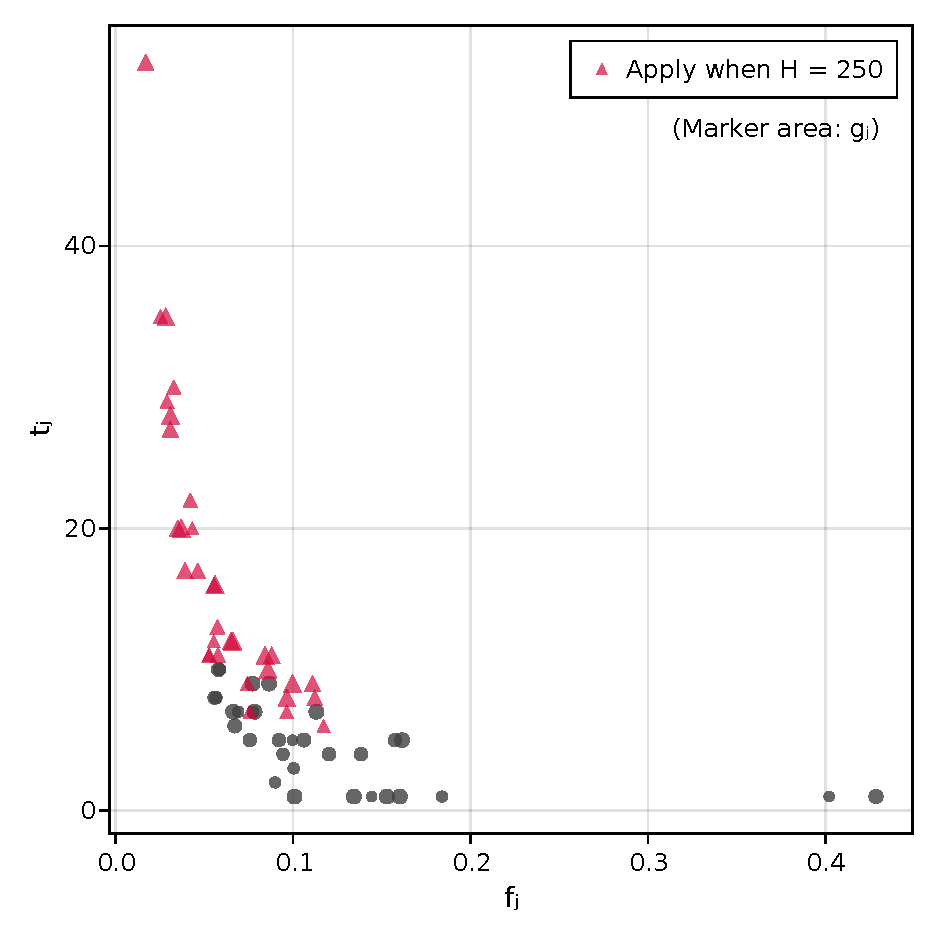
\includegraphics[width=0.85\textwidth]{./plots/samplemarket.pdf}
  \caption{\label{samplemarket}
 \ifen A typical randomly-generated instance with $m=64$ schools and its optimal application portfolio. The application costs $g_j$ were drawn uniformly from $\{5, \dots, 10\}$. The optimal portfolio was computed using Algorithm \ref{ellisDP1}.
 \else $m=64$개의 학교로 구성된 전형적인 무작위로 생성한 인스턴스와 해당 최적 포트폴리오. 지원 비용 $g_j$는 $\{5, \dots, 10\}$에서 균일한 확률로 선정했으며 기호의 넓이와 비례된다. 최적 포트폴리오는 알고리즘 \ref{ellisDP1}(으)로 계산했다. \fi}
\end{figure}


\begin{table}[h!] \centering
\small
\begin{tabular}{r|r@{~}r|r@{~}r}
\ifen 
 \textbf{\begin{tabular}[r]{@{}r@{}}Number of\\schools $m$\end{tabular}}& \multicolumn{2}{c|}{\textbf{\begin{tabular}[c]{@{}c@{}}Algorithm \ref{algorithmforlargeh}\\with array\end{tabular}}}  & \multicolumn{2}{c}{\textbf{\begin{tabular}[c]{@{}c@{}}Algorithm \ref{algorithmforlargeh}\\with heap\end{tabular}}}\\ \hline
 \else
 \textbf{\begin{tabular}[r]{@{}r@{}}학교의\\개수 $m$\end{tabular}}& \multicolumn{2}{c|}{\textbf{\begin{tabular}[c]{@{}c@{}}알고리즘 \ref{algorithmforlargeh}\\(배열 구현)\end{tabular}}}  & \multicolumn{2}{c}{\textbf{\begin{tabular}[c]{@{}c@{}}알고리즘 \ref{algorithmforlargeh}\\(힙 구현)\end{tabular}}}\\ \hline
 \fi
    16 &    0.00 &  (0.00) &    0.01 &    (0.00) \\
    64 &    0.01 &  (0.00) &    0.08 &    (0.02) \\
   256 &    0.06 &  (0.00) &    0.96 &    (0.26) \\
  1024 &    0.82 &  (0.03) &   14.27 &    (2.28) \\
  4096 &   12.87 &  (0.71) &  230.77 &   (18.75) \\
 16384 &  199.48 &  (1.77) & 3999.19 &  (283.48)
\end{tabular}
\caption{\label{experiment1results} \normalsize
\ifen (Experiment 1.) Time in ms to compute an optimal portfolio for an admissions market with homogeneous application costs using Algorithm \ref{algorithmforlargeh} when $\mathcal{C}$ is stored as an array and as a heap. \lastptofcaption~In every case, $h = m/2$. 
\else (실험 1.) 단위: ms. 알고리즘 \ref{algorithmforlargeh}에서 $\mathcal{C}$를 배열 또는 힙 구현으로 저장했을 때, 
동일 지원 비용 입학 시장의 최적 지원 포트폴리오를 계산하는 시간. \lastptofcaption~모든 경우, $h = m/2$. \fi}
\end{table}






\begin{table}[h!] \centering
\small
\begin{tabular}{r|r@{~}r|r@{~}r|r@{~}r|r@{~}r}
\ifen
\textbf{\begin{tabular}[r]{@{}r@{}}Number of\\schools $m$\end{tabular}}&\multicolumn{2}{c|}{\textbf{\begin{tabular}[c]{@{}c@{}}Algorithm \ref{ellisbnb}:\\Branch \& bound\end{tabular}}}  & \multicolumn{2}{c|}{\textbf{\begin{tabular}[c]{@{}c@{}}Algorithm \ref{ellisDP1}:\\Costs DP\end{tabular}}}  &\multicolumn{2}{c|}{\textbf{\begin{tabular}[c]{@{}c@{}}Algorithm \ref{ellisDP3}:\\FPTAS, $\varepsilon= 0.5$\end{tabular}}}  & \multicolumn{2}{c}{\textbf{\begin{tabular}[c]{@{}c@{}}Algorithm \ref{ellisDP3}:\\FPTAS, $\varepsilon= 0.05$\end{tabular}}}   \\ \hline
\else
\textbf{\begin{tabular}[r]{@{}r@{}}학교의\\개수 $m$\end{tabular}}&\multicolumn{2}{c|}{\textbf{\begin{tabular}[c]{@{}c@{}}알고리즘  \ref{ellisbnb}:\\분지한계법\end{tabular}}}  & \multicolumn{2}{c|}{\textbf{\begin{tabular}[c]{@{}c@{}}알고리즘 \ref{ellisDP1}:\\지출액 동적 계획\end{tabular}}}  &\multicolumn{2}{c|}{\textbf{\begin{tabular}[c]{@{}c@{}}알고리즘 \ref{ellisDP3}:\\FPTAS, $\varepsilon= 0.5$\end{tabular}}}  & \multicolumn{2}{c}{\textbf{\begin{tabular}[c]{@{}c@{}}알고리즘 \ref{ellisDP3}:\\FPTAS, $\varepsilon= 0.05$\end{tabular}}}   \\ \hline
\fi
   8 &  0.02 & (0.01) &  0.01 & (0.00) &   0.05 &   (0.01) &     0.16 &    (0.04) \\
  16 &  0.10 & (0.04) &  0.07 & (0.02) &   0.39 &   (0.10) &     2.59 &    (0.62) \\
  32 & 12.43 & (9.88) &  0.29 & (0.05) &   2.15 &   (0.29) &    33.07 &   (10.72) \\
  64 &     — &    (—) &  1.24 & (0.16) &  13.24 &   (2.22) &   339.64 &  (100.38) \\
 128 &     — &    (—) &  6.20 & (0.64) &  79.92 &  (20.18) &  2042.63 &  (749.71) \\
 256 &     — &    (—) & 30.63 & (2.28) & 818.50 & (632.98) & 18949.50 & (3533.88)
\end{tabular}%
\caption{\label{experiment2results} \normalsize
\ifen (Experiment 2.) Time in ms to compute an optimal or $(1 - \varepsilon)$-optimal portfolio for an admissions market with heterogeneous application costs using the three algorithms developed in Section \ref{hetappcosts}.
%branch-and-bound routine (Algorithm \ref{ellisbnb}), exact dynamic program (Algorithm \ref{ellisDP1}), and the fully polynomial-time approximation scheme (Algorithm \ref{ellisDP3}).
The branch-and-bound algorithm is impractical for large markets. \lastptofcaption
\else  %분지한계법 (알고리즘 \ref{ellisbnb}), 정확한 동적 계획 (알고리즘 \ref{ellisDP1}), 그리고 완전 다항 시간 근사 해법 (알고리즘 \ref{ellisDP3})을
(실험 2.) 단위: ms. \ref{hetappcosts}절에서 도출한 3개의 알고리즘을 사용할 때, 다양한 지원 비용으로 갖춘 입학 시장의 최적 또는 $(1- \varepsilon)$-최적 포트폴리오를 계산하는 시간. 분지한계법은 큰 시장에서 비실용적이다. \lastptofcaption \fi}
\end{table}




\begin{figure}[h!] 
\centering
%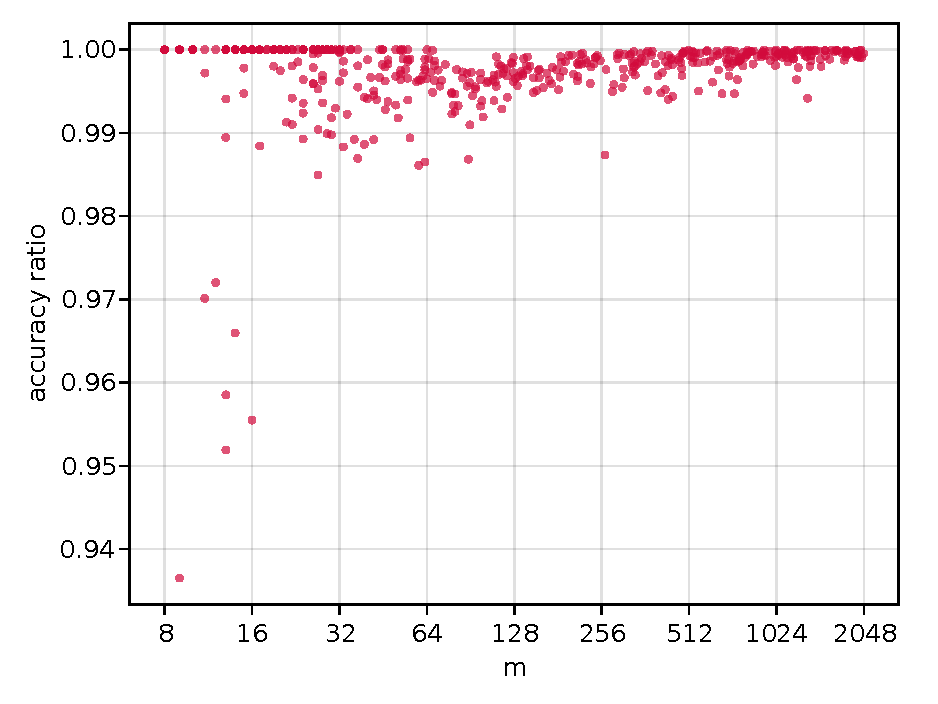
\includegraphics[width=0.95\textwidth]{./plots/accuracy_simulatedannealing.pdf}
  \caption{\label{experiment3results}
 \ifen (Experiment 3.) Optimality ratio achieved by simulated annealing (Algorithm \ref{ellissimann}) in markets of varying size, with parameters $N = 500$, $T = 1/4$, and $r = 1/16$. Optimal portfolios were computed using Algorithm \ref{ellisDP1}. 
 \else  (실험 3.) 크기가 다양한 시장에 적용한 모의 담금질 (알고리즘 \ref{ellissimann}) 해법이 달성하는 최적성 비율. 모의 담금질의 모수는 $N = 500, T = 1/4, r = 1/16$이며, 최적 포트폴리오는 알고리즘 \ref{ellisDP1}(으)로 계산했다. \fi}
\end{figure}








%\pagebreak
\ifen \section{Conclusion and ideas for future research} \else \section{결론과 향후 연구}\fi\label{conclusion}
\ifen
This study has introduced a novel combinatorial optimization problem that we call the college application problem. It can be viewed as a kind of asset allocation or knapsack problem with a submodular objective. We showed that the special case in which colleges have identical application costs can be solved in polynomial time by a greedy algorithm because the optimal solutions are nested in the budget constraint. The general problem is NP-complete. We provided four solution algorithms. The strongest from a theoretical standpoint is an FPTAS that produces a $(1-\varepsilon)$-approximate solution in $O(m^3 / \varepsilon)$ time. On the other hand, for typical college-application instances, the dynamic program based on application expenditures is both easier to implement and substantially more time efficient. A heuristic simulated-annealing algorithm also exhibited strong empirical performance in our computational study. The algorithms discussed in this paper are summarized in Table \ref{algorithmssummary}.
\else
본 연구는 새로운 조합 최적화 문제를 제안했으며 이를 대학 입학 지원 최적화 문제라고 부른다. Submodular한 목적함수를 가지는 자산 배분 혹은 배낭 문제로 볼 수 있다. 모든 대학의 지원 비용이 동일한 특수한 경우, 탐욕 알고리즘으로 다항 시간에 풀 수 있음을 보였으며 최적해가 예산 제약식에 대한 포함 사슬 관계를 가지기 때문이다. 일반적인 문제는 NP-complete하다. 4가지 해법을 제시했으며 이론적으로 가장 효율적인 알고리즘은 $O(m^3 / \varepsilon)$ 시간에  $(1-\varepsilon)$-근사해를 계산하는 FPTAS다. 그 반면에 전형적인 대학 지원 문제 인스턴스에 대해, 지원 비용 지출액 기반 동적 계획 해법은 실행하기 쉬울뿐더러 계산 시간이 상당히 짧다. 계산 실험에서 모의 담금질 기반 휴리스틱 해법도 좋은 성능을 발휘했다. 표 \ref{algorithmssummary}에서 본 논문이 다운 알고리즘을 정리한다.
\fi

\ifen
\begin{table}[h!] \centering
\small
\begin{tabular}{r|lllll}
\textbf{Algorithm} & \textbf{Reference}  & \textbf{Problem} & \textbf{Restrictions} & \textbf{Exactness}       & \textbf{Computation time} \\ \hline
\xrowht[()]{1.5em}  \begin{tabular}[r]{@{}r@{}}Na\"ive\end{tabular} & Definition \ref{naivealgorithm}                   & \begin{tabular}[l]{@{}l@{}}Homogeneous \\ costs\end{tabular}     & None                  & $(1/h)$-opt.               & $O(m)$                    \\ 
\xrowht[()]{1.5em}  Greedy                & Algorithm \ref{algorithmforlargeh} &  \begin{tabular}[l]{@{}l@{}}Homogeneous \\ costs\end{tabular}    & None                  & Exact                    & $O(hm)$                   \\
\xrowht[()]{1.5em}  \begin{tabular}[r]{@{}r@{}}Branch and\\ bound\end{tabular}   & Algorithm \ref{ellisbnb} & General          & None                  & Exact                    & $O(2^m)$                  \\
\xrowht[()]{1.5em}  Costs DP     &  Algorithm \ref{ellisDP1}& General          & $g_j$ integer         & Exact                    & $O(Hm + m \log m)$        \\
\xrowht[()]{1.5em}  FPTAS      &    Algorithm \ref{ellisDP3} & General          &  None         & $(1 - \varepsilon)$-opt. & $O(m^3 / \varepsilon)$   \\
\xrowht[()]{1.5em}  \begin{tabular}[r]{@{}r@{}}Simulated\\annealing\end{tabular}        &    Algorithm \ref{ellissimann} & General          &  None         & $0$-opt. & $O(Nm)$   
\end{tabular}%
\caption{\label{algorithmssummary} \normalsize
Summary of algorithms discussed in this paper.}
\end{table}
\else
\begin{table}[h!] \centering
\small
\begin{tabular}{r|lllll}
\textbf{알고리즘} & \textbf{논문 내 위치}  & \textbf{문제} & \textbf{제한} & \textbf{정확도}       & \textbf{계산 시간} \\ \hline
\xrowht[()]{1.7em}  \begin{tabular}[r]{@{}r@{}}나이브\end{tabular} & 정의 \ref{naivealgorithm}                   & \begin{tabular}[l]{@{}l@{}}동일한\\ 지원 비용\end{tabular}     & 없음                  & $(1/h)$-근사          & $O(m)$                    \\ 
\xrowht[()]{1.7em}  탐욕 해법                & 알고리즘 \ref{algorithmforlargeh} &  \begin{tabular}[l]{@{}l@{}}동일한\\ 지원 비용\end{tabular}    & 없음                  & 정확                    & $O(hm)$                   \\
\xrowht[()]{1.7em}  \begin{tabular}[r]{@{}r@{}}분지한계법\end{tabular}   & 알고리즘 \ref{ellisbnb} & 일반 문제          & 없음                  & 정확                    & $O(2^m)$                  \\
\xrowht[()]{1.7em}   \begin{tabular}[r]{@{}r@{}}지출액\\ 동적 계획\end{tabular}     &  알고리즘 \ref{ellisDP1}& 일반 문제          & $g_j$ 정수         & 정확                    & $O(Hm + m \log m)$        \\
\xrowht[()]{1.7em}  FPTAS      &    알고리즘 \ref{ellisDP3} & 일반 문제          &  없음    & $(1 - \varepsilon)$-근사 & $O(m^3 / \varepsilon)$   \\
\xrowht[()]{1.7em}  모의 담금질      &    알고리즘  \ref{ellissimann} & 일반 문제          &  없음    & $0$-근사 & $O(Nm)$   
\end{tabular}%
\caption{\label{algorithmssummary} \normalsize
본 논문에서 다룬 해법의 요약.}
\end{table}
\fi

\ifen 
Three extensions of this problem appear amenable to future study.
\else
이 문제를 확장할 수 있는 향후 연구 방향 3가지를 제안할 수 있다. 
\fi


\ifen \subsection{Explicit treatment of risk aversion}\else \subsection{위험 회피를 모수화한 모형}\fi
\ifen
The familiar Markowitz portfolio optimization model includes an explicit risk-aversion term, whereas our model has settled for an implicit treatment of risk, namely the tradeoff between selective schools and safety schools inherent in the maximax objective function. However, it is possible to augment the objective function $v(\mathcal{X}) = \operatorname{E}[X]$ to incorporate a variance penalty $\beta \geq 0$ as follows:
\else
익숙한 Markowitz 포트폴리오 최적화 모형에서는 명시적인 위험 회피 항이 등장하며, 본 모형은 maximax 목적함수에 내포된 경쟁적인 학교와 안정 지원 학교 사이의 균형에 의한 위험 관리 요소만 고려했다. 그러나 기본 목적함수인 $v(\mathcal{X}) = \operatorname{E}[X]$에 표준편차 페널티 $\beta \geq 0$를 다음처럼 도입할 수 있다:
\fi
\begin{align}
\begin{split}
v_{\mathrm{\beta}}(\mathcal{X}) &=  \operatorname{E}[X] - \beta \operatorname{Var}(X) \\
&=   \operatorname{E}[X] - \beta \left(  \operatorname{E}[X^2]  -  \operatorname{E}[X]^2 \right) \\
& = \sum_{j\in\{0\}\cup\mathcal{X}} \Bigl( f_j t_j \prod_{\substack{i \in \mathcal{ ̄X}: \\ i > j}} (1 - f_{i}) \Bigr)
 - \beta \sum_{j\in\{0\}\cup\mathcal{X}} \Bigl( f_j t_j^2 \prod_{\substack{i \in \mathcal{X}: \\ i > j}} (1 - f_{i}) \Bigr)
  + \beta v(\mathcal{X})^2 \\
  &= v(\mathcal{X}; \tau) +  \beta v(\mathcal{X}; t)^2
\end{split}
\end{align}
\ifen
where $\tau_j = t_j - \beta t_j^2$. Since the first term is itself a portfolio valuation function, and the second is a monotonic transformation of one, we speculate that one of the algorithms given above could be used as a subroutine to trace out the efficient frontier by maximizing $v(\mathcal{X}; t)$ subject to the budget constraint and $v(\mathcal{X}; \tau) \geq \alpha$ for various values of $\alpha \geq 0$. 
\else
단, $\tau_j = t_j - \beta t_j^2$. 이의 첫 번째 항 그 자체가 포트폴리오 가치 함수이며, 두 번째 항은 포트폴리오 가치 함수의 단조 변환이다. 따라서 위에서 제시한 알고리즘을 서브루틴으로 사용하면 효율적 투자선(efficient frontier)을 탐색할 수 있어 보인다. 이때 다양한 $\alpha \geq 0$에 대해 예산 제약식과 $v(\mathcal{X}; \tau) \geq \alpha$ 아래서 $v(\mathcal{X}; t)$을 최대화하는 것이 알고리즘의 요점이다.
\fi

\ifen
A parametric treatment of risk aversion may align our model more closely to real-world applicant behavior. Conventional wisdom asserts that the best college application strategy combines reach, target, and safety schools in roughly equal proportion (Jeon 2015). When the application budget is small relative to the size of the admissions market, our algorithms recommend a similar approach (see the example of Subsection \ref{planetsexamplesection}). However, inspecting equation \eqref{howtotransformtj}, which discounts school utility parameters to reflect their marginal value relative to the schools already in the portfolio, reveals that low-utility schools are penalized more harshly than high utility schools in the marginal analysis. Consequentially, as the application budget grows, the optimal portfolio in our model tends to favor reach schools over safety schools. (See Figure \ref{samplemarket} for a clear illustration of this phenomenon.)
 
A potential application of our model is an econometric study that estimates students’ perceptions of college quality ($t_j$) from their observed application behavior ($\mathcal{X}$) under the assumption of utility maximization. Empirical research indicates that heterogeneous risk aversion is a significant source of variation in human decision-making, especially in the domains of educational choice and employment search (Kahneman 2011; Hartlaub and Schneider 2012; van Huizen and Alessie 2019). Therefore, an endogenous risk-aversion parameter would greatly enhance our model’s explanatory power in the econometric setting.
\else
위험 회피를 모수화한 모형은 실제 지원 행동을 더 정확하게 반영할 수 있다. ``상향·소신·안정'' 지원 학교를 대략 균일하게 분산하여 지원하는 것이 최적이란 통념이다 (전민희 2015). 입학 시장의 크기에 비해 지원 예산이 작은 경우, 본 연구에서 제시하는 알고리즘은 비슷한 전략을 추천한다 (항 \ref{planetsexamplesection}의 예제 참고). 그러나 포트폴리오에 이미 삽입한 학교를 반영한 한계 가치를 나타내도록 효용 모수를 할인하는 수식 \eqref{howtotransformtj}을 살펴보면, 효용이 높은 학교보다 효용이 낮은 학교에 부과되는 페널티가 큰 것을 알 수 있다. 그 결과는 지원 예산이 커질수록 본 모형의 최적 포트폴리오가 안정 지원 학교보다 상향 지원 학교를 편드는 것이다. (그림 \ref{samplemarket}에서 뚜렷이 보이는 현상이다.)

학생의 지원 행동($\mathcal{X}$)을 관찰하고 학생이 인식하는 대학교의 질($t_j$)을 추정하는 경제 측정학 연구에서 본 논문의 모형을 그대로 응용할 수 있다. 실무 연구 결과에 따르면 위험 회피의 다양성은 인간 의사 결정 다양성의 주된 원인이 되며, 교육 선택과 취업 활동은 특히 그렇다 (Kahneman 2011; Hartlaub와 Schneider 2012; van Huizen과 Alessie 2019). 따라서 경제 측정학 맥락에서, 위험 회피 모수를 내생 변수로 도입하면 원래 모형의 묘사력을 많이 개선할 수 있다.
\fi

\ifen \subsection{Signaling strategies and matroid constraints}\else \subsection{시그널 전략과 matroid 제약 조건}\fi
\ifen
Another direction of further research with immediate application in college admissions is to incorporate additional signaling strategies into the problem. In the Korean admissions process, the online application form contains three multiple-choice fields, labeled \emph{ga, na,} and \emph{da} for the first three letters of the Korean alphabet, which students use to indicate the colleges to which they wish to apply. Most schools appear only in one or two of the three fields. Therefore, students are restricted not only in the number of applications they can submit, but in the combinations of schools that may coincide in a feasible application portfolio. From a portfolio optimization perspective, this is a \emph{diversification constraint,} because its primary purpose is to prevent students from applying only to top-tier schools. However, in addition to overall selectivity, the three fields also indicate different evaluation schemes: The \emph{ga} and \emph{na} customarily indicate the applicant's first and second choice, and applications filed under these fields are evaluated with greater emphasis on standardized-test scores than those filed under the \emph{da} field. Some colleges appear in multiple fields and run two parallel admissions processes, each with different evaluation criteria. Therefore, if a student recognizes that she has a comparative advantage in (for example) her interview skills, she may increase her chances of admission to a competitive school by applying under the \emph{da} field. The optimal application strategy in this context can be quite subtle, and it is a subject of perennial debate on Korean social networks.

An analogous feature of the American college admissions process is known as early decision, in which at the moment of application, a student commits to enrolling in a college if admitted. In principle, students who apply with early decision may obtain a better chance of admission by signaling their eagerness to attend, but doing so weakens the college's incentive to entice the student with discretionary financial aid, altering the utility calculus.
\else
향후 연구에 두 번째 방향은 모형에 시그널 전략을 도입하는 것이다. 한국 정시 입학 과정의 온라인 지원 양식에는 가군, 나군, 다군이란 3가지 선다형 칸을 채워서 지원하는 학교를 선택한다. 대부분의 학교는 모든 3개의 칸에 등장하지 않고 그중 1~2개만 가능하다. 따라서 학생이 지원할 수 있는 학교의 `수'일 뿐만 아니라 가능한 지원 포트폴리오에 같이 들어갈 수 있는 학교의 `조합'도 제한된다. 이는 학생이 상위권 대학만 지원하지 않도록 만들어지기 때문에 다각화(diversification) 제약식으로 볼 수 있다. 그러나 대학이 어떤 군에 속하는 것은 대학 순위일뿐더러 입학 전형 유형도 의미한다. 가군과 나군은 관례적으로 학생이 선호하는 대학을 선택하는 것이며 다군보다 수능 점수의 반영 비율이 높은 편이다. 또한 군 2개에 포함되는 학교도 있으며 입학 전형이 다르면서 평행한 모집 과정 2개를 운영한다. 가령, 어떤 학생이 면접 능력에 비교 우위가 있으면 경쟁적인 학교에 다군으로 지원하면 합격 확률을 높일 수도 있다. 이런 맥락에서 최적의 지원 전략은 미묘한 문제이며 한국 SNS에서 자주 발생하는 화젯거리다.

미국 입학 과정의 유사한 특징은 조기 전형(early decision)이라고 불린다. 이는 학생이 합격하면 진학한다고 약속하고 지원하는 것을 의미한다. 조기 전형으로 지원하면 입학할 관심을 시그널할 수 있으므로 합격 확률을 높일 수 있지만, 학교가 학생을 모집하려고 장학금을 수여할 동기가 약화할 수 있으므로 학생의 효용 추정이 달라진다.
\fi


\ifen
In the integer formulation of the college application problem (Problem \ref{integernlp}), a natural way to model these signaling strategies without introducing too much complexity is to split each $c_j$ into $c_{j+}$ and $c_{j-}$. The binary decision variables are $x_{j+} = 1$ if the student applies to $c_j$ with high priority (that is, in  the \emph{ga} or \emph{na} field or with early decision) and $x_{j-} = 1$ if applying with low priority (that is, in the \emph{da} field or without early decision). Now, assuming that the differential admission probabilities $f_{j+}$ and $f_{j-}$ and utilities $t_{j+}$ and $t_{j-}$ are known, adding the logical constraints 
\begin{align}
 x_{j+} + x_{j-} \leq 1, ~~ j = 1\dots m\qquad\text{and}\qquad\sum_{j=1}^m x_{j+} \leq 1
\end{align}
completes the formulation. These are knapsack constraints; therefore, the submodular maximization algorithm of Kulik et al. (2013) can be used to obtain a $(1 - 1/e - \varepsilon)$-approximate solution to this problem. When the budget constraint is a cardinality constraint (as in Alma's problem), we note that imposing the signaling constraints yields a matroidal solution set, and Calinescu et al. (2011)'s algorithm yields an alternative solution, which has the same approximation coefficient of $1 - 1/e -\varepsilon$. %These constraints are conformable to those of the multiple knapsack problem (Kellerer et al. 2004, chap. 10).
\else
대학 지원 문제의 정수 모형(문제 \ref{integernlp})에서 위의 시그널 전략들을 어렵지 않게 도입하는 방식은 각 $c_j$를 $c_{j+}$와 $c_{j-}$로 나누는 것이다. 그다음에 학생이 $c_j$에 높은 관심을 시그널하면 (즉, 가군으로 선택하거나 조기 전형으로 지원하면) $x_{j+} = 1$이며 관심을 시그널 하지 않고 지원하면 (즉 가군 혹은 나군으로 지원하거나 조기 전형 없이 지원하면) $x_{j-} = 1$이 되는 이진 결정 변수를 정의한다. 해당 합격 확률 $f_{j+}$와 $f_{j-}$ 그리고 효용  $t_{j+}$와 $t_{j-}$가 알려져 있으면, 다음 같은 논리 제약식을 더하면 모형을 완성할 수 있다. 
\begin{align}
 x_{j+} + x_{j-} \leq 1, ~~ j = 1\dots m\qquad\text{그리고}\qquad\sum_{j=1}^m x_{j+} \leq 1
\end{align}
모두 배낭 제약식이므로 Kulik 외 (2013)의 submodular 최대화 알고리즘을 통해 이 문제의 $(1 - 1/e - \varepsilon)$-근사해를 구할 수 있다. 또한 (알마의 문제처럼) 예산 제약식이 집합 크기 제약식이 되면, 논리 제약식을 더한 모형의 해집합이 matroid가 되며, Calinescu 외 (2011)의 알고리즘이 대안 해법이 된다. 단, 그의 근사 계수는 여전히 $1 - 1/e - \varepsilon$이다. 
\fi

\ifen 
Our main results indicate that the objective function of the college application problem, though nonlinear, has similar regularity properties to a linear function: The greedy algorithm finds the maximum over a cardinality constraint, and an FPTAS exists for maximization over a knapsack constraint. For linear functions, however, the greedy algorithm is optimal over matroid constraints as well (Edmonds 1971). Thus, if the pseudolinearity of our objective function is sufficiently robust, the greedy algorithm will be an exact solution for the college application with matroid constraints, including the signaling constraints discussed above. Preliminary numerical experiments suggest that this is the case, but the class of matroids is diverse and difficult to test exhaustively. (The nestedness property does not apply automatically to matroids because in the proof of the elimination technique given in \S\,\ref{eliminationtechniquesection}, we assumed that $\mathcal{X} \cup \{k\}$ implies the feasibility of $\mathcal{Y} \cup \{k\}$ when $|\mathcal{X}| = |\mathcal{Y}|$.)
\else
본 연구의 주된 결과는 대학 지원 문제의 목적함수가 선형 함수가 아니지만, 최적화 관점에서 선형 함수와 비슷한 성질을 가진다는 것으로 해석할 수 있다. 집합 크기 제약 아래서 탐욕 해법이 정확하고, 배낭 제약 아래서 FPTAS가 존재하기 때문이다. 그런데 선형 함수는 matroid 제약 아래서 최적화하는 문제도 탐욕 해법으로 풀 수 있다 (Edmonds 1971). 따라서 대학 지원 목적함수와 선형 함수의 유사성이 적당히 깊으면 위에서 논한 matroid 제약 아래서 이를 최대화하는 문제를 탐욕 해법으로 풀 수 있을 것이다. 예비 수리 실험을 진행한 결과로 이 성질이 사실처럼 보이지만, matroid가 아주 광범위한 클래스이므로 철저한 실험이 어렵다. (\S\,\ref{eliminationtechniquesection}에서 제시된 변수 기법의 증명 과정에서 $|\mathcal{X}| = |\mathcal{Y}|$일 때 $\mathcal{X} \cup \{k\}$가 가능해면 $\mathcal{Y} \cup \{k\}$도 가능해라고 가정하기 때문에 포함 사슬 관계 성질을 matroid에 자동으로 확장할 수 있는 것이 아니다.)
\fi



\ifen \subsection{Memory-efficient dynamic programs}\else \subsection{동적 계획의 메모리 소요 절감}\fi
\ifen
Our numerical experiments suggest that the performance of the dynamic programming algorithms is bottlenecked by not computation time, but memory usage. Reducing these algorithms' storage requirements would enable us to solve considerably larger problems.

Abstractly speaking, Algorithms \ref{ellisDP1} and \ref{ellisDP3} are two-dimensional dynamic programs that represent the optimal solution by $Z[N, C]$. Here $N$ is the number of decision variables, $C$ is a constraint parameter, and $Z[n, c]$ is the optimal objective value achievable using the first $n\leq N$ decision variables when the constraint parameter is $c \leq C$. The algorithm iterates on a recursion relation that expresses $Z[n, c]$ as a function of $Z[n -1, c]$ and $Z[n -1, c']$ for some $c' \leq c$. (In Algorithm \ref{ellisDP1}, $Z$ is the maximal portfolio valuation, $N = m$, and $C =H$; in Algorithm \ref{ellisDP3},  $Z$ is the minimal application expenditures, $N = m$, and $C = |\mathcal{V}| \propto m^2 / \varepsilon$.)

When such a dynamic program is implemented using a lookup table or dictionary memoization, producing the optimal solution requires $O(NC)$ time and space. Kellerer et al. (2004, \S\,3.3) provide a technique for transforming the dynamic program $Z$ into a divide-and-conquer algorithm that produces the optimal solution in $O(N C)$ time and $O(N + C)$ space, a significant improvement. However, their technique requires the objective function to be additively separable in a certain sense that appears difficult to conform to the college application problem. 
\else
수리 실험 결과에 따르면 동적 계획 해법 성능의 병목 요소는 계산 시간이 아니라 메모리 소모량이다. 이 알고리즘의 메모리 소요를 절감하면 상당히 큰 문제를 풀 수 있다.

추상적인 관점에서, 알고리즘 \ref{ellisDP1}과(와) 알고리즘 \ref{ellisDP3}은(는) 최적해를 $Z[N, C]$로 표현하는 2차원 동적 계획이다. 이때 $N$은 결정 변수의 수, $C$는 제약식의 모수, 그리고 $Z[n, c]$는 제약 모수가 $c \leq C$일 때 첫 $n\leq N$개의 결정 변수만 이용하는 최적 목적 함숫값이다. 알고리즘의 구조는 $Z[n, c]$를 $Z[n -1, c]$와 어떤 $c' \leq c$에 대응하는 $Z[n -1, c']$의 함수로 표현하고 그 반복 관계로 탐색하는 것이다. (알고리즘 \ref{ellisDP1}에서 $Z$는 최대 포트폴리오 가치, $N = m$, 그리고 $C =H$이며, 알고리즘 \ref{ellisDP3}에서 $Z$는 최소한 지원 지출액, $N = m$, 그리고 $C= |\mathcal{V}| \propto m^2 / \varepsilon$이다.)

이러한 형태의 동적 계획을 표 혹은 사전 기록으로 구현하면 최적해를 출력하는 것은 $O(NC)$ 시간과 $O(NC)$ 공간을 소요한다. Kellerer 외 (2004, \S\,3.3)는 동적 계획 $Z$를 $O(N C)$ 시간과 $O(N + C)$ 공간 안에 최적해를 구하는 분할 정복(divide and conquer) 알고리즘으로 변환하는 일반적인 방법을 제시하며 매우 유익하다. 그러나 이를 이용할 수 있는 조건 중, 목적함수는 어떤 기술적인 의미에서 가산적으로 분할되어야 하며 이를 대학 지원 문제에 적용하기 어렵다.
\fi

\appendix
\ifen \section{Appendix} \else \section{부록} \fi

\ifen \subsection{Elementary proof of Theorem \ref{concavityinh}} \else \subsection{정리 \ref{concavityinh}의 기초적 증명} \fi \label{elementaryconcavityproof}
\begin{proof}
\ifen We will prove the equivalent expression $2 v(\mathcal{X}_h) \geq v(\mathcal{X}_{h+1}) + v(\mathcal{X}_{h-1})$. Applying Theorem \ref{nestedapplication}, we write $\mathcal{X}_h = \mathcal{X}_{h-1} \cup\{j\}$ and $\mathcal{X}_{h+1} = \mathcal{X}_{h-1} \cup\{j, k\}$. If $t_k \leq t_j$, then 
\else $2 v(\mathcal{X}_h) \geq v(\mathcal{X}_{h+1}) + v(\mathcal{X}_{h-1})$ 같은 동등한 부등식을 증명하자. 정리 \ref{nestedapplication}을(를) 적용하면 $ \mathcal{X}_h = \mathcal{X}_{h-1} \cup\{j\}$ 그리고 $\mathcal{X}_{h+1} = \mathcal{X}_{h-1} \cup\{j, k\}$으로 표현할 수 있다. $t_k \leq t_j$인 경우, \fi
\begin{align}
\begin{split}
2 v(\mathcal{X}_h) &= v(\mathcal{X}_{h-1} \cup\{j\}) + v(\mathcal{X}_{h-1} \cup\{j\}) \\
&\geq v(\mathcal{X}_{h-1} \cup\{k\}) + v(\mathcal{X}_{h-1} \cup\{j\}) \\
&= v(\mathcal{X}_{h-1} \cup\{k\}) + (1 - f_j) v(\mathcal{X}_{h-1}) + f_j \operatorname{E}[\max\{t_j, X_{h-1}\}] \\
&= v(\mathcal{X}_{h-1} \cup\{k\}) - f_j v(\mathcal{X}_{h-1}) + f_j \operatorname{E}[\max\{t_j, X_{h-1}\}] + v(\mathcal{X}_{h-1})  \\
&\geq v(\mathcal{X}_{h-1} \cup\{k\})  - f_j v(\mathcal{X}_{h-1}\cup\{k\}) + f_j \operatorname{E}[\max\{t_j, X_{h-1}\}]+ v(\mathcal{X}_{h-1})\\
&= (1 - f_j) v(\mathcal{X}_{h-1} \cup\{k\})  + f_j \operatorname{E}[\max\{t_j, X_{h-1}\}]+ v(\mathcal{X}_{h-1})\\
&=  v(\mathcal{X}_{h-1} \cup\{j, k\}) + v(\mathcal{X}_{h-1})\\
&=  v(\mathcal{X}_{h+1}) + v(\mathcal{X}_{h-1}).
\end{split} 
\end{align}
\ifen The first inequality follows from the optimality of $\mathcal{X}_h$, while the second follows from the fact that adding $k$ to $\mathcal{X}_{h-1}$ can only increase its valuation.
\else 첫 번째 부등식은 $\mathcal{X}_h$의 최적성에 따르며, 두 번째 부등식은 $\mathcal{X}_{h-1}$에 $j$를 더하면 가치가 증가할 수밖에 없기 때문이다.\fi

\ifen If $t_k \geq t_j$, then the steps are analogous:
\else  $t_k \geq t_j$인 경우는 유사하다:\fi
\begin{align}
\begin{split}
2 v(\mathcal{X}_h) &= v(\mathcal{X}_{h-1} \cup\{j\}) + v(\mathcal{X}_{h-1} \cup\{j\}) \\
&\geq v(\mathcal{X}_{h-1} \cup\{k\}) + v(\mathcal{X}_{h-1} \cup\{j\}) \\
&= (1 - f_k) v(\mathcal{X}_{h-1}) + f_k \operatorname{E}[\max\{t_k, X_{h-1}\}] +  v(\mathcal{X}_{h-1} \cup\{j\})  \\
&= v(\mathcal{X}_{h-1}) - f_k  v(\mathcal{X}_{h-1}) + f_k \operatorname{E}[\max\{t_k, X_{h-1}\}] +  v(\mathcal{X}_{h-1} \cup\{j\})  \\
&\geq v(\mathcal{X}_{h-1}) - f_k  v(\mathcal{X}_{h-1}\cup\{j\}) + f_k \operatorname{E}[\max\{t_k, X_{h-1}\}] +  v(\mathcal{X}_{h-1} \cup\{j\})  \\
&= v(\mathcal{X}_{h-1}) + (1 - f_k) v(\mathcal{X}_{h-1}\cup\{j\}) + f_k \operatorname{E}[\max\{t_k, X_{h-1}\}]  \\
&= v(\mathcal{X}_{h-1}) + v(\mathcal{X}_{h-1} \cup\{j, k\})
\end{split}\\
&= v(\mathcal{X}_{h-1})  + v(\mathcal{X}_{h+1}) \qedhere
\end{align}
\end{proof}



\iffalse

\subsection{Generalization of Theorem \ref{nestedapplication} for matroid constraints} \label{matroidnestedapplicationheader}

\begin{definition}[Matroid]
Consider a ground set $\mathcal{C}$ and a collection $\mathfrak{I}$ of subsets of $\mathcal{C}$, the system $(\mathcal{C}, \mathfrak{I})$ is called a \emph{matroid} if and only if the following three condtions hold:
\begin{enumerate}
\item $\varnothing \in \mathfrak{I}$.
\item $\mathfrak{I}$ is downward-closed: $\mathcal{X} \in \mathfrak{I}$ and $ \mathcal{Y} \subseteq \mathcal{X}$ implies $\mathcal{Y} \in \mathfrak{I}$.
\item If $\mathcal{X} \in \mathfrak{I}$ and $|\mathcal{Y}| < |\mathcal{X}|$, then there is an element $k \in \mathcal{X}$ such that $\mathcal{Y} \cup \{k\} \in \mathfrak{I}$. 
\end{enumerate}
The elements of $\mathfrak{I}$ are called the \emph{independent sets} of the matroid; subsets of $\mathcal{C}$ that are not independent are called \emph{dependent}. If $\mathcal{X}$ is an independent set such that $\mathcal{X} \cup \{j\} \notin \mathfrak{I}$ for all $j \in\mathcal{C} \setminus \mathcal{X}$, then $\mathcal{X}$ is called \emph{base} of $(\mathcal{C}, \mathfrak{I})$. %The third property implies that all bases have the same cardinality, called the matroid's \emph{rank.}
\end{definition}


\begin{problem}[\ifen Alma’s problem with matroid constraints\else 매트로이드 제약이 있는 알마의 문제\fi]
%\ifen Alma's optimal college application portfolio is given by the solution to the following combinatorial optimization problem:
%\else
%알마의 최적 대학 지원 포트폴리오는 다음 조합 최적화 문제의 최적해다.
%\fi
\begin{align}
\begin{split}
\text{maximize}\quad &  v(\mathcal{X}) = \sum_{j\in
%\{0\}\cup
\mathcal{X}} \Bigl( f_j t_j \prod_{\substack{i \in \mathcal{X}: \\ i > j}} (1 - f_{i}) \Bigr)\\
\text{subject to}\quad & \mathcal{X} \in \mathfrak{I}
\end{split}
\end{align}
where $\mathcal{C}, \mathfrak{I})$ is a matroid.
\end{problem}



\begin{definition}[Greedy algorithm for Alma's problem with matroid constraints]
At each iteration, add to $\mathcal{X}$ the school $k$ for which $v(\mathcal{X} \cup \{k\})$ is greatest and $\mathcal{X} \in $
\end{definition}

%\begin{theorem}
%
%\end{theorem}
\else



















\pagebreak
\ifen
\section*{References}
\addcontentsline{toc}{section}{References}
\else
\section*{참고문헌}
\addcontentsline{toc}{section}{참고문헌}
\fi
\noindent


% Add to bib: Gale and Shapley 1962 Roth 1982, , Azevedo and Leshno 2016 Bodoh-Creed 2020; Ashlagi and Nikzad 2020, Kapur 2021




\end{document}  

